% ALT 2027 submission. Keep alt2027.cls, jmlr.cls and jmlrutils.sty next to
% this file. Compiler: pdfLaTeX (Overleaf default).
\documentclass[anon]{alt2027} % submission (anonymized)
%\documentclass[final]{alt2027} % camera-ready (de-anonymized)

% Loaded by the class: amsmath, amssymb, natbib, graphicx, url, xcolor,
% hyperref, algorithm2e (environment algorithm2e), and theorem, lemma,
% proposition, corollary, definition, remark, conjecture, example and proof
% environments. The class refuses amsthm.
\usepackage{times}
\usepackage[T1]{fontenc}
\usepackage{booktabs}
\usepackage{multirow}
\usepackage{microtype}
\usepackage{enumitem}
\usepackage{needspace}

% Revision marks: every new or rewritten passage is printed in color.
% Set \revmarksfalse to print the whole paper in black.
\newif\ifrevmarks\revmarkstrue
\definecolor{revcolor}{RGB}{0,84,166}
\newenvironment{revised}{\ifrevmarks\color{revcolor}\fi}{}
\newcommand{\rev}[1]{{\ifrevmarks\color{revcolor}\fi#1}}

% The class numbers theorems, lemmas, propositions, corollaries, definitions
% and remarks with one shared counter. Give lemmas, propositions,
% corollaries, definitions and remarks their own counters, so that the
% numbering reads Theorem 1, 2, 3, Lemma 1, 2, ... Delete this block to go
% back to the shared counter.
\makeatletter
\newcommand{\altrenumber}[2]{%
  \expandafter\let\csname #1\endcsname\relax
  \expandafter\let\csname end#1\endcsname\relax
  % newer LaTeX (Overleaf) already defines \the<name>; clear it so the new
  % counter's numbering is used instead of the shared theorem number
  \expandafter\let\csname the#1\endcsname\relax
  \expandafter\let\csname theH#1\endcsname\relax
  \newtheorem{#1}{#2}}
\makeatother
\altrenumber{lemma}{Lemma}
\altrenumber{proposition}{Proposition}
\altrenumber{corollary}{Corollary}
\theorembodyfont{\upshape}
\altrenumber{definition}{Definition}
\altrenumber{remark}{Remark}
\theorembodyfont{\itshape}
\altrenumber{observation}{Observation}
\providecommand{\qed}{\hfill\jmlrBlackBox}
% allow slightly loose lines rather than lines that run into the margin
\setlength{\emergencystretch}{3em}

% The class puts a theorem's title inside the list label, which cannot break
% across lines, so long titles ran into the margin. Same look, but the title
% is set as ordinary text and can wrap.
\makeatletter
\renewcommand*{\@opargbegintheorem}[3]{%
  \ifdef{\@jmlr@currentthm}%
  {%
    \letcs{\jmlr@this@theoremheader}{jmlr@thm@\@jmlr@currentthm @header@font}%
    \letcs{\jmlr@this@theorembody}{jmlr@thm@\@jmlr@currentthm @body@font}%
    \letcs{\jmlr@this@theoremsep}{jmlr@thm@\@jmlr@currentthm @sep}%
    \letcs{\jmlr@this@theorempostheader}%
       {jmlr@thm@\@jmlr@currentthm @postheader}%
  }%
  {%
    \let\jmlr@this@theorembody\@theorembodyfont
    \let\jmlr@this@theoremheader\@theoremheaderfont
    \let\jmlr@this@theoremsep\@theoremsep
    \let\jmlr@this@theorempostheader\@theorempostheader
  }%
  \trivlist
   \item[\hskip\labelsep{\jmlr@this@theoremheader #1\ #2}]%
   {\jmlr@this@theoremheader (#3)\jmlr@this@theorempostheader}\ %
   \mbox{}\jmlr@this@theoremsep
   \jmlr@this@theorembody
}
\makeatother

% Blackboard bold sets
\newcommand{\R}{\mathbb{R}}
\newcommand{\N}{\mathbb{N}}
\newcommand{\Z}{\mathbb{Z}}
\newcommand{\Q}{\mathbb{Q}}
\newcommand{\C}{\mathbb{C}}

% Labels
\newcommand{\alg}{\mathrm{alg}}
\newcommand{\meta}{\mathrm{meta}}
\newcommand{\fix}{\mathrm{fix}}

% Probability
\newcommand{\Prb}{\mathbb{P}}
\newcommand{\E}{\mathbb{E}}
\DeclareMathOperator{\Var}{Var}
\DeclareMathOperator{\Cov}{Cov}

% Operators
\DeclareMathOperator{\diag}{diag}
\DeclareMathOperator{\supp}{supp}

\newcommand{\argmax}{\operatorname*{arg\,max}}
\newcommand{\argmin}{\operatorname*{arg\,min}}
\newcommand{\ind}{\mathbf{1}}

% Inner product
\newcommand{\inner}[2]{\left\langle #1, #2 \right\rangle}

% Calligraphic sets
\newcommand{\cA}{\mathcal{A}}
\newcommand{\cS}{\mathcal{S}}
\newcommand{\cT}{\mathcal{T}}
\newcommand{\cF}{\mathcal{F}}
\newcommand{\cE}{\mathcal{E}}

% RL notation
\newcommand{\SSS}{\mathcal{S}}
\newcommand{\AAA}{\mathcal{A}}
\newcommand{\PP}{\mathcal{P}}
\newcommand{\RRR}{\mathcal{R}}
\newcommand{\gammaRL}{\gamma}

% Confidence bounds
\newcommand{\olQ}{\overline{Q}}
\newcommand{\ulQ}{\underline{Q}}
\newcommand{\olV}{\overline{V}}
\newcommand{\ulV}{\underline{V}}

% Misc
\newcommand{\eps}{\varepsilon}
\newcommand{\dt}{\mathrm{d}t}
\newcommand{\given}{\,\bigl\vert\,}

% Fractions
\newcommand{\half}{\tfrac12}
\newcommand{\thalf}{\tfrac32}

% Notes
\newcommand{\note}[1]{\paragraph{Note.} #1}



\newcommand{\todo}[1]{\textcolor{red!70!black}{[\textbf{TODO:} #1]}}
\newcommand{\Cold}{\mathsf{C}}
\newcommand{\Exp}{\mathsf{E}}
\newcommand{\Hyb}{\mathsf{H}}
\newcommand{\wid}{w}

\title[Information Value Is Not Policy Value]{Information Value Is Not Policy Value:\\ When LLM Warm-Starts Help Linear Contextual Bandits}
% Alternative title that names the main idea (see the change list):
% \title[Where the Right Answers Fall]{Where the Right Answers Fall:\\ When LLM Warm Starts Help Linear Contextual Bandits}

% Hidden by the [anon] option. Fill in for the camera-ready version.
\altauthor{%
 \Name{Author Name1} \Email{abc@sample.com}\\
 \addr Address 1
 \AND
 \Name{Author Name2} \Email{xyz@sample.com}\\
 \addr Address 2%
}

\begin{document}
\maketitle
\begin{abstract}
\begin{revised}
Large language models (LLMs) carry broad knowledge about the world, and a
natural use of it is to guide systems that learn from feedback, such as an
online store that learns which category to assign to each new product. A
simple recipe lets a fixed, pretrained LLM make the first decisions of a
linear contextual bandit and then hands control to the bandit algorithm
LinUCB. This combination can beat both the LLM and LinUCB on their own, yet
the LLM's accuracy does not predict when it does. We show that an expert's
value to the learner is decided by where its correct answers fall, and not
by how many correct answers it gives. The expert's data reaches the learner
in two ways: through \emph{coverage}, the directions of the feature space
that its actions explore, and through the \emph{transfer}, what its rewards
reveal beyond that coverage. We prove that with the exploration that
LinUCB's theory requires, coverage is all that matters under linear rewards,
and its value is capped by a ratio of prices, a cap that is tight up to a
constant factor. With the smaller exploration used in practice, we prove
that a few rewarded answers on a frequently correct action make LinUCB
commit to that action. Two experts with the same coverage, cost and number
of correct answers can then differ in value by a factor that grows with the
time horizon, and the more accurate expert can be the worse one. On a large
product-categorization benchmark, removing the transfer removes every
significant difference between three LLM experts, and the gain disappears
when the learner explores more or when no category is frequent.
\end{revised}
\end{abstract}

\begin{keywords}%
linear contextual bandits, LinUCB, warm start, large language models, exploration, regret
\end{keywords}


\section{Introduction}
\label{sec:intro}

\begin{revised}
Many online systems must learn from feedback which action to take in each
situation. An online store, for example, must assign each new product page
to one of thousands of categories, and it learns whether a choice was right
only after making it. The \emph{contextual bandit} is the standard model of
this problem \citep{lattimore2020bandit}. At each round a learner sees a
context, such as a product description, chooses an action, such as a
category, and observes the reward of that action only. Large language
models (LLMs) bring broad prior knowledge to such problems, because they can
read the context and propose a reasonable action before any feedback
arrives \citep{brown2020language,ouyang2022training,achiam2023gpt}.

A simple way to combine the two is to let a fixed, pretrained LLM, which we
call the \emph{expert}, choose the actions of the first rounds, and then to
hand control to LinUCB, the standard upper-confidence-bound algorithm for
linear contextual bandits \citep{li2010contextual,chu2011contextual}.
LinUCB learns from every round, including the rounds the expert played.
\citet{chen2024llmdecision} and \citet{huangcontextual} found that such
combinations can beat both the LLM alone and LinUCB started from scratch,
which we call \emph{cold} LinUCB. The LLM's accuracy is a poor guide to this
gain. On the AmazonCat-13K product-categorization benchmark, three LLM
experts that are right on only $3.6$--$5.3\%$ of products raise the accuracy
of the same learner by factors of $1.71$ to $3.29$, and the least accurate
expert is not the least useful (Section~\ref{sec:experiments}).

This paper explains where the gain comes from and why accuracy cannot
predict it. Our main finding is the following: \emph{when LinUCB explores as
it does in practice, an expert's value to the learner is decided by where
its correct answers fall, and not by how many correct answers it gives.} A
correct answer on an action that pays often, such as a category that fits a
third of all products, can make the learner commit to that action for the
rest of the run. The same number of correct answers spread over rarely
correct actions cannot. The information that an expert's data carries
therefore does not determine its value to the learner's policy, which is
the sense of our title.
\end{revised}

\begin{revised}
To make this precise, we separate the two ways in which the expert's rounds
affect LinUCB. The first is \emph{coverage}. Each action the expert plays
informs LinUCB about one direction of the feature space, and the more often
a direction is played, the less uncertain LinUCB is about the actions along
it. In the store example, coverage records which kinds of products and
categories the learner has already tried. The second is the
\emph{transfer}, which is what the rewards of those rounds tell LinUCB
beyond their coverage. If the expert chooses a category exactly on the
products where it is correct, the rewards show that this category often
pays, which coverage alone cannot show. Which of the two channels matters
depends on how much LinUCB explores (Table~\ref{tab:map}).
\end{revised}

\begin{revised}
With the exploration that LinUCB's regret guarantees require, coverage is
never free. To cover a direction, a policy must play actions along it, and
those actions cost regret. Cold LinUCB buys the same coverage on its own. We
prove that the saving coverage can provide is therefore at most the ratio of
the prices that the two policies pay for it, and that this cap is attained
up to a constant factor (Section~\ref{sec:price}). When rewards are linear
in the features with independent noise, coverage is moreover all that the
expert's data provides. On AmazonCat, however, the three experts cover the
same directions to within $5\%$, at nearly the same prices, and their gains
differ severalfold.
\end{revised}

\begin{revised}
Practical implementations of LinUCB explore much less than its guarantees
require, and so do the experiments in which the gains were observed. In
this regime, we prove that a few rewarded answers on an action that pays
often make LinUCB \emph{settle} on that action, that is, keep choosing it,
with a failure probability that is exponentially small in a margin set by
those answers (Section~\ref{sec:two-channels}). Two experts with the same
coverage, the same cost and the same number of correct answers can then
have values that differ by a factor that grows with the horizon, and the
more accurate expert can be the worse one. This holds for a fixed handoff
and for the adaptive rule of our experiments, which we call the
\emph{Router}.
\end{revised}

\begin{table}[t]
\begin{revised}
\centering
\caption{Map of the results. Which channel can produce a gain depends on how
much LinUCB explores.}
\label{tab:map}
\small
\begin{tabular}{@{}p{0.12\linewidth}p{0.40\linewidth}p{0.40\linewidth}@{}}
\toprule
& Exploration the theory requires & Reduced exploration, as in practice\\
\midrule
Coverage & Saving capped by a price ratio, and the cap is attained up to a
constant. It is all there is under linear rewards (Section~\ref{sec:price}).
& Small on AmazonCat: $2$ to $3.5\%$ of cold LinUCB's regret, the same for
every expert (Section~\ref{sec:amazon}).\\
\addlinespace
Transfer & Cannot make LinUCB settle while untried actions are offered
(Section~\ref{sec:two-channels}). & Decides settling. Separates experts with
equal coverage, cost and correct answers (Section~\ref{sec:two-channels}).
Carries every significant difference on AmazonCat (Section~\ref{sec:amazon}).\\
\bottomrule
\end{tabular}
\end{revised}
\end{table}

\begin{revised}
Experiments on AmazonCat-13K confirm each of these predictions
(Section~\ref{sec:experiments}). Coverage alone saves $2$ to $3.5\%$ of cold
LinUCB's regret, the same for every expert. The transfer carries the rest of
the gain and every significant difference between experts. It acts through
one category that is correct on $29.8\%$ of products. A few rewarded routed
answers on this category decide whether LinUCB settles there, and the same
answers with their rewards hidden give no gain. The gain disappears when
LinUCB explores more and when that category is made rarer.
\end{revised}

\begin{revised}
Our contributions are as follows.
\begin{itemize}[itemsep=1pt,topsep=2pt,leftmargin=*]
\item We prove that, when LinUCB explores less than its theory requires, two
experts that leave the same coverage, have the same cost and give the same
number of correct answers can make LinUCB's regret differ by a factor that
grows with the horizon. This holds for a fixed handoff and for the Router,
and already in three dimensions (Section~\ref{sec:two-channels}).
\item We prove that rewarded answers before the handoff make LinUCB settle on
an action with a failure probability that is exponentially small in a margin
that these answers set. We extend this result to features that change with
the context (Section~\ref{sec:two-channels} and
Appendix~\ref{app:settling-context}).
\item We prove that, with the exploration that LinUCB's theory requires, the
saving coverage can provide over cold LinUCB is capped by a ratio of prices,
and we show that the cap is attained up to a constant factor
(Section~\ref{sec:price}).
\item We show on AmazonCat-13K, with OneShotWikiLinks as a control that has
no frequent label, that the transfer carries the gain and every significant
difference between experts, with all settings tuned on held-out seeds
(Section~\ref{sec:experiments}).
\end{itemize}
Section~\ref{sec:setup} sets up the model and the two channels, and all
proofs are in the appendix.
\end{revised}

\begin{revised}
Our work is closest to methods that combine an LLM with a contextual bandit.
\citet{chen2024llmdecision} run the LLM and a bandit learner side by side
and choose between them with an online model-selection algorithm.
\citet{huangcontextual}, \citet{jumpstart2026} and \citet{calibgated2026}
use the LLM's uncertainty, preferences or pseudo-observations to start or
steer LinUCB. These works propose combination rules and analyze them through
the quality of the LLM's predictions. We instead determine which part of the
expert's data produces the gain, and we show that accuracy cannot predict
it. Our decomposition and price bound hold for any set of routed rounds, so
they apply to all of these rules. Model-selection methods such as CORRAL
\citep{agarwal2017corralling} compete with the best of several base
learners, and we determine when a combination beats all of them. Analyses of
warm starts from logged data \citep{zhang2019warm} and of
hybrid offline-to-online reinforcement learning
\citep{song2022hybrid,wagenmaker2023leveraging} value the data by its
quality or coverage and treat it as free. We charge for acquiring it.
\citet{bastani2021mostly} also observed that a learner that explores little
can lock onto whichever action paid first. We show that, for an online warm
start, this makes the value of an expert's data depend on where its correct
answers fall. Work on misspecified linear bandits
\citep{ghosh2017misspecified,lattimore2020learning,foster2020adapting}
treats the part of the reward that the linear model misses as a cost. Here
that part, carried by the transfer, is the main source of the gain.
Appendix~\ref{sec:related} compares with further work.
\end{revised}

\section{Setup and the Two Channels}
\label{sec:setup}
\label{sec:preliminaries}

\begin{revised}
We work in the standard linear contextual bandit. At each round
$t=1,\dots,T$ the learner observes a finite set of actions $\mathcal A_t$.
Each action $a\in\mathcal A_t$ comes with a feature vector
$x_{t,a}\in\R^d$, $\|x_{t,a}\|_2\le L$, which describes the pair of context
and action. In AmazonCat, for example, it combines the embedding of the
product text with that of the category name. The learner selects
$A_t\in\mathcal A_t$ and observes the reward
$r_t=\langle\theta^\star,x_{t,A_t}\rangle+\eta_t$, where $\theta^\star$ is
an unknown parameter with $\|\theta^\star\|_2\le S$ and $\eta_t$ is noise
with conditional mean zero and $\sigma$-sub-Gaussian tails ($\sigma=\frac12$
for rewards in $[0,1]$). Write $\mu_t(a)=\langle\theta^\star,x_{t,a}\rangle$
for the mean reward of $a$ and $\Delta_{t,a}=\max_b\mu_t(b)-\mu_t(a)$ for
its \emph{gap}. The \emph{regret} of a policy $\pi$ on an interval
$I\subseteq[T]$ is the total gap of the actions it plays,
$R_I(\pi)=\sum_{t\in I}\Delta_{t,\pi_t}$, and $R_T(\pi)=R_{[T]}(\pi)$. The
\emph{regret ratio} of $\pi$ over cold LinUCB is $R_T(\Cold)/R_T(\pi)$, so a
ratio above $1$ means that $\pi$ does better.
\end{revised}

\begin{revised}
LinUCB keeps the \emph{design matrix}
$V_t=V_1+\sum_{s<t}x_{s,A_s}x_{s,A_s}^\top$, the \emph{response sum}
$c_t=c_1+\sum_{s<t}r_sx_{s,A_s}$ and the estimate
$\widehat\theta_t=V_t^{-1}c_t$. It plays an action of largest index,
$A_t\in\arg\max_a\langle\widehat\theta_t,x_{t,a}\rangle+\beta_t\|x_{t,a}\|_{V_t^{-1}}$.
Here $\|x\|_{V^{-1}}=\sqrt{x^\top V^{-1}x}$ is the \emph{width} of $x$,
which measures how uncertain LinUCB is about the reward of $x$, and the
\emph{confidence radius} $\beta_t$ sets how much LinUCB explores. We call the
radius \emph{valid} if, with high probability,
$\|\widehat\theta_t-\theta^\star\|_{V_t}\le\beta_t$ at every round. LinUCB's
regret guarantees hold for valid radii, such as the radius of
\citet{abbasi2011improved}, which grows like $\sqrt{d\log T}$. Practical
implementations use much smaller radii. \emph{Cold} LinUCB, $\Cold$, starts
from $V_1=\lambda I_d$ and $c_1=0$. A \emph{warm start} $(M,c)$ starts from
$V_1=\lambda I_d+M$ and $c_1=c$, where $M=\sum_sx_sx_s^\top$ and
$c=\sum_sr_sx_s$ are the Gram matrix and the response sum of some earlier
data. A frozen expert $\Exp$ proposes an action $a_t^{\Exp}$ by a rule that
never changes. For an LLM, this is the action whose embedding is closest to
the LLM's output. The \emph{handoff hybrid} $\Hyb_\tau$ plays $a_t^{\Exp}$
for $t\le\tau$, feeds every played action and reward to $(V_t,c_t)$, and
plays LinUCB for $t>\tau$. Its LinUCB phase is thus LinUCB with the
\emph{online} warm start $(M_\tau,c_\tau)$ that the routed rounds leave, and
the cost of those rounds counts toward the regret. The \emph{Router} of our
experiments (Appendix~\ref{app:meta-algorithm}) instead decides at every
round whether the expert or LinUCB acts, choosing whichever is more
confident about its proposal.
\end{revised}

\begin{revised}
To see where the hybrid's gain comes from, we split it into what happens
during the routed rounds and what happens after them.
\end{revised}
\label{sec:decomp}

\begin{proposition}[Decomposition identity]
\label{prop:decomp}
For any instance, expert, $\tau$ and realization of the noise,
\begin{align*}
R_T(\Cold)-R_T(\Hyb_\tau)
&=\underbrace{R_{[1,\tau]}(\Cold)-R_{[1,\tau]}(\Exp)}_{A_\tau}
 +\underbrace{R_{[\tau+1,T]}(\Cold)-R_{[\tau+1,T]}(\Hyb_\tau)}_{I_\tau},\\
R_T(\Exp)-R_T(\Hyb_\tau)
&=\underbrace{R_{[\tau+1,T]}(\Exp)-R_{[\tau+1,T]}(\Hyb_\tau)}_{B_\tau}.
\end{align*}
\end{proposition}

\begin{revised}
Here $A_\tau$ is the expert's direct advantage on the routed rounds,
$I_\tau$ is the \emph{tail value} of the data those rounds leave, since both
runs face the same future from different starting states, and $B_\tau$ is
the learner's advantage over the expert afterwards. We call
$R_{[1,\tau]}(\Exp)$ the \emph{acquisition regret} of the warm start. The
identities hold for every realization, and also when the routed rounds are
chosen adaptively, as by the Router (Remark~\ref{rem:decomp}).
\end{revised}

\begin{revised}
A warm start enters LinUCB through two objects. The design matrix
$V_1=\lambda I+M$ fixes every width, and the response sum $c_1=c$ fixes the
estimate. The \emph{coverage} of a direction $u$ by played actions $x_s$ is
$\sum_s\langle x_s,u\rangle^2$, the growth of the design matrix along $u$.
Widths along $u$ fall only as this coverage grows
(Lemma~\ref{lem:loewner}). With a valid radius, LinUCB plays a suboptimal
action only while $2\beta_t$ times its width is at least its gap
(Lemma~\ref{lem:width-limited}). We say that a design matrix
\emph{certifies} an action once this fails, because the confidence bound
alone then rules the action out.

The rewards of the routed rounds act through the response sum, and they can
say more than coverage does. The reward can depart from the linear model,
$r(x)=\langle\theta^\star,x\rangle+\varepsilon(x)+\eta$, for a reference
parameter $\theta^\star$ and a residual $\varepsilon$ that the linear model
misses. The binary rewards of our experiments are of this form, with a large
residual. An LLM also reads the raw context, so it can prefer an action on
exactly the rounds where that action pays. In either case the estimate at
the handoff gains a term that the Gram matrix does not determine. We call it
the \emph{transfer},
\begin{equation}
\label{eq:transfer}
m:=V_1^{-1}\sum_{s\le\tau}\bigl(r_s-\langle\theta^\star,x_s\rangle\bigr)\,x_s,
\qquad\text{so that}\qquad
\widehat\theta_1=\theta^\star-\lambda V_1^{-1}\theta^\star+m
\end{equation}
exactly. Given $M$, the transfer is the only part of the estimate at the
handoff that depends on which rounds were routed and what they returned.
Section~\ref{sec:price} determines what coverage can provide when LinUCB's
radius is valid, and Section~\ref{sec:two-channels} what the transfer adds
when it is not.
\end{revised}

\section{Valid Exploration: Coverage and Its Price}
\label{sec:price}

\begin{revised}
This section assumes that LinUCB's radius is valid, so that its confidence
event holds. Coverage then has a price, because the only way to cover a
direction is to play actions along it. For a direction $u$, the
\emph{price}
\end{revised}
\begin{equation}
\label{eq:price}
\kappa_t(u):=\min\Bigl\{\frac{\Delta_{t,a}}{\langle x_{t,a},u\rangle^2}:\ a\in\mathcal A_t,\ \langle x_{t,a},u\rangle\neq0\Bigr\},
\qquad \kappa(u):=\inf_t\kappa_t(u),
\end{equation}
\begin{revised}
is the least regret that any policy pays at round $t$ per unit of coverage
of $u$. No policy, expert or otherwise, obtains coverage for less. Its
coverage of $u$ over any interval is at most its regret there divided by
$\kappa(u)$ (Lemma~\ref{lem:no-free-coverage}). Cold LinUCB buys coverage on
its own, because optimism makes it pull each arm whose width exceeds its gap
until it no longer does. The value of an expert's coverage is therefore set
by the prices that each side pays.
\end{revised}

\begin{revised}
To state the bound, let $\mathcal X\subset\R^d$ be a finite set of arms with
$\|x\|_2\le L$ and let $\mathcal A_t\subseteq\mathcal X$. Suppose that an
arm of maximal mean belongs to every $\mathcal A_t$, so that each arm has a
fixed gap $\Delta(x)$. Let $\mathcal S$ be the suboptimal arms and
$\beta\ge\beta_t$ for all $t\le T$. Cold LinUCB covers $u_x:=x/\|x\|_2$ by
pulling $x$ itself, at price $\kappa_x:=\Delta(x)/\|x\|_2^2$. For a policy
$\pi$ playing arms $x^\pi_t$ and a cutoff $t_0$, write
$\mathrm{cov}(y):=\sum_{x\in\mathcal S}\langle y,u_x\rangle^2$, and let
$\kappa^\pi(t_0):=\min\{\Delta(x^\pi_t)/\mathrm{cov}(x^\pi_t):t\le t_0,\
\Delta(x^\pi_t)>0,\ \mathrm{cov}(x^\pi_t)>0\}$ be the price that $\pi$ pays.
\end{revised}

\begin{theorem}[Price bound, simple form]
\label{thm:general-price}
On the confidence event of cold LinUCB, let $\pi$ be any policy and $t_0$ a
cutoff such that the design matrix of $\pi$'s first $t_0$ rounds certifies
every arm of $\mathcal S$, and such that the optimal arms $\pi$ plays before
$t_0$ are orthogonal to every arm of $\mathcal S$. With the price ratio
$P:=\max_{x\in\mathcal S}\kappa_x/\kappa^\pi(t_0)$,
\[
R_T(\Cold)\ \le\ P\,R_{[1,t_0]}(\pi)+\sum_{x\in\mathcal S}\Delta(x),
\qquad\text{so}\qquad
\frac{R_T(\Cold)}{R_T(\pi)}\ \le\ P+\frac{\sum_{x\in\mathcal S}\Delta(x)}{R_T(\pi)}.
\]
\end{theorem}

\begin{revised}
Theorem~\ref{thm:general-price-full} in Appendix~\ref{app:moved} gives the
general form, for any set of certified arms, with a residual equal to cold
LinUCB's regret on the arms that $\pi$ did not pay to rule out. The bound
uses only cold LinUCB's confidence event and allows any $\pi$, so it covers
the fixed-handoff hybrid, the Router and model-selection masters such as
CORRAL alike. It is also tight up to a constant factor.
Theorem~\ref{thm:price} (Appendix~\ref{app:template-thm}) constructs, for
every value of the price ratio, an instance with a cheap \emph{probe}, a
nearly optimal action along a direction that recurs. On this instance the
hybrid that routes the probes beats cold LinUCB by the price ratio up to a
constant factor, and beats the expert by a factor that grows with $T$.
Coverage alone can therefore give a large gain, but only when the expert has
an action of small gap along a direction that cold LinUCB can cover only
with actions of large gap.
\end{revised}

\begin{revised}
When rewards are linear and the noise is independent of the routing,
coverage is all that the expert's data provides.
\end{revised}

\begin{observation}[Coverage is complete under linear rewards]
\label{prop:response-sum}
\label{cor:coverage-complete}
Let the warm start be built from $(x_s,r_s)_{s\le\tau}$ with
$r_s=\langle\theta^\star,x_s\rangle+\eta_s$, the $\eta_s$ i.i.d.\
$\mathcal N(0,\sigma^2)$ and independent of which actions were logged and
which rounds were routed, and let the later contexts be independent of the
routed data. Then $c=M\theta^\star+\xi$ with $\xi\sim\mathcal N(0,\sigma^2M)$
given $M$, so two experts that leave the same Gram matrix leave warm starts
with the same law, and their hybrids have the same expected tail value.
\end{observation}

\begin{revised}
The Router violates these assumptions, because it routes based on past
rewards, so Section~\ref{sec:amazon} tests the conclusion directly. Under
valid exploration and linear rewards, coverage is thus all that the
expert's data contributes, and prices cap its value. Neither conclusion
describes AmazonCat. There, the experts' measured price ratios are small and
nearly equal ($1.73$, $1.59$ and $1.58$), yet their gains differ
severalfold.
\end{revised}

\section{Reduced Exploration: The Transfer}
\label{sec:two-channels}

\begin{revised}
Practical LinUCB explores less than its theory requires. This section shows
that the transfer then decides whether LinUCB settles on an action, and
that settling separates experts that coverage cannot tell apart.
\end{revised}

\begin{table}[t]
\centering
\caption{The instance of Theorem~\ref{thm:transfer-separation}: for each round
type, how often it occurs, which action pays, and what each expert plays.}
\label{tab:instance}
\small
\begin{tabular}{@{}lcccc@{}}
\toprule
Round type & $D$ & $R$ & $F$ & $\varnothing$\\
\midrule
Rounds in the window ($t\le4k$) & $k$ & $k$ & $0$ & $2k$\\
Probability after the window & $p$ & $q$ & $f$ & $1-p-q-f$\\
Action with reward $1$ & $D$ & $R$ & fresh arm $b_t$ & none\\
$\Exp_A$ plays & $D$ (right) & $D$ & $D$ & $R$\\
$\Exp_B$ plays & $R$ & $R$ (right) & $b_t$ (right) & $D$\\
\bottomrule
\end{tabular}
\end{table}

\begin{revised}
After the handoff, LinUCB \emph{settles} on an action $a$ if it plays $a$ at
every later round. While LinUCB keeps playing $a$, its estimate of $a$ is a
running average of $a$'s rewards. If that average never drops below what the
best competitor can offer, LinUCB never leaves $a$. The rewarded answers
before the handoff set where the average starts, and this is how the
transfer enters. Formally, fix an action $a$ offered at every round with the
same unit feature $u$, and let LinUCB, with a constant radius $\beta>0$,
play every round after $\tau$ from any warm start. The other features are
arbitrary. With $V:=V_{\tau+1}$ and $\widehat\theta:=\widehat\theta_{\tau+1}$
the state at the handoff, let $N:=1/\|u\|^2_{V^{-1}}$,
$\widehat\mu_a:=\langle\widehat\theta,u\rangle$ and $s:=N\widehat\mu_a$.
Then $a$'s width is $1/\sqrt N$ and its estimate is $s/N$, so $N$ acts as a
count of plays and $s$ as their total reward. For a competing feature $x$,
let $\rho(x):=\langle x,V^{-1}u\rangle/\|u\|^2_{V^{-1}}$ be its overlap with
$u$ in LinUCB's geometry and
$I(x):=\langle\widehat\theta,x\rangle+\beta\|x\|_{V^{-1}}$ its index at the
handoff. With the offered sets fixed in advance and every
$\rho(x_{t,b})<1$, define the \emph{threshold} and the \emph{margin}
\[
\omega:=\max_{\tau<t\le T}\ \max_{b\in\mathcal A_t\setminus\{a\}}
\frac{I(x_{t,b})-\rho(x_{t,b})\,\widehat\mu_a}{1-\rho(x_{t,b})},
\qquad h:=N(\widehat\mu_a-\omega).
\]
An estimate of $a$ above $\omega$ beats every competitor at every round, and
$h$ measures how far $a$'s estimate starts above $\omega$, in units of data.
In the \emph{orthogonal case}, every other feature, offered or in the data,
is orthogonal to $u$, as in any finite-armed bandit. Then $\rho\equiv0$,
$\omega$ is the largest competing index, $N=\lambda+n$ with $n$ the number
of plays of $a$, and $s$ is the reward they returned. Given the past, $a$'s
reward after $\tau$ has mean at least $\mu_a$ and $\sigma$-sub-Gaussian
deviations.
\end{revised}

\begin{theorem}[Settling under a constant radius]
\label{thm:settling}
Given the handoff state:
\begin{enumerate}[itemsep=1pt,topsep=1pt,leftmargin=*]
\item[(i)] If $\mu_a>\omega$ and $h>0$, then with probability at least
$1-e^{-2(\mu_a-\omega)h/\sigma^2}$ LinUCB plays $a$ at every round after
$\tau$.
\end{enumerate}
In the orthogonal case, moreover:
\begin{enumerate}[itemsep=1pt,topsep=1pt,leftmargin=*]
\item[(ii)] If $a$'s index at handoff is below some $\omega_-$ and some competitor
always has index at least $\omega_-$, LinUCB never plays $a$ after $\tau$.
\rev{If the plays of $a$ returned no reward, or their rewards are hidden, then
$s=0$ and $a$'s index $\beta/\sqrt{\lambda+n}$ is below its cold value
$\beta/\sqrt\lambda$.}
\item[(iii)] If $a$'s rewards are i.i.d.\ Bernoulli$(\mu_a)$, the largest competing
index stays $\omega>\beta/\sqrt{\lambda+n}$ and $T$ is long enough, LinUCB
fails to settle with probability at least $(1-\mu_a)^j$, where
$j=\bigl\lfloor(h+\beta\sqrt{\lambda+n})/(\omega-\beta/\sqrt{\lambda+n})\bigr\rfloor+1$.
\end{enumerate}
\end{theorem}

\begin{revised}
The margin is where the transfer enters. A play of $a$ with reward $1$
raises $s$ by exactly one, and a play of $a$ without reward lowers $h$ by
$\omega$. In the orthogonal case, parts (i) and (iii) show that LinUCB fails
to settle with probability $e^{-\Theta(h)}$ from both sides. A handful of
rewarded answers therefore decides, and settling is close to all or
nothing. Part (i) needs no orthogonality.
Appendix~\ref{app:settling-context} extends it to features that change with
the context, as in our experiments, where a category's feature $x_t\odot
z_a$ differs for every product. There, each play moves LinUCB's estimate
along a reference direction as a play of the reference feature would,
discounted by how well LinUCB already knows the rest of the feature
(Theorem~\ref{thm:settling-context}).
\end{revised}

\begin{revised}
We now show that settling, and not coverage, can decide the regret ratio.
The next result is a separation result, not a model of AmazonCat. It makes
everything that coverage can see equal and shows that the outcome still
differs. Fix $k\ge1$, $0\le q<p$ and $0\le f<p$ with $p+q+f\le1$, $L>1$,
$\lambda>0$, $T>4k$ and $d=T+2$. At round $t$ the learner is offered
$D=e_1$, $R=e_2$ and a fresh arm $b_t=Le_{t+2}$. Each round has a type that
the learner does not see, and the type decides which action has reward $1$
(Table~\ref{tab:instance}). The first $\tau:=4k$ rounds form a window, and
later types are i.i.d. In the store example, $D$ is a category that fits
many products, $R$ one that fits few, and the fresh arms are the many rarely
correct categories that cold LinUCB keeps trying. Regret is pseudo-regret
against $\theta^\star=pe_1+qe_2+(f/L)\sum_te_{t+2}$, so the gaps are $0$ for
$D$, $p-q$ for $R$ and $p-f$ for each $b_t$. Correct answers are counted on
the realized types. Two experts see the type. After the window, $\Exp_A$ is
right with probability $p$ and $\Exp_B$ with probability $q+f$, so $\Exp_B$
is the more accurate whenever $f>p-q$. LinUCB uses a constant radius
$\beta$, and $\omega:=\beta L/\sqrt\lambda$ is the index of an untried fresh
arm. Ties go to the fresh arm. In the window each expert plays $D$ and $R$
exactly $2k$ times and is right exactly $k$ times. Only where their correct
answers fall differs.
\end{revised}

\begin{theorem}[Equal coverage, unequal value]
\label{thm:transfer-separation}
On this instance:
\begin{enumerate}[itemsep=1pt,topsep=1pt,leftmargin=*]
\item[(i)] $M_\tau^{A}=M_\tau^{B}=2k(e_1e_1^\top+e_2e_2^\top)$, both acquisition
regrets are $2k(p-q)$, each expert is right on $k$ routed rounds, and the
estimates at handoff differ only through the transfer,
$\widehat\theta^{A}_{\tau+1}=\frac{k}{\lambda+2k}e_1$ and
$\widehat\theta^{B}_{\tau+1}=\frac{k}{\lambda+2k}e_2$.
\item[(ii)] Cold LinUCB plays the fresh arm at every round, so
$R_T(\Cold)=(p-f)T$, and so does either hybrid after $\tau$ if the routed
rounds contribute their covariance but not their rewards.
\item[(iii)] $\Hyb^{B}_\tau$ never plays $D$ after $\tau$, so
$R_T(\Hyb^{B}_\tau)\ge(T-2k)\min\{p-q,p-f\}$.
\item[(iv)] If $\omega<p$ and $h:=k(1-2\omega)-\omega\lambda>0$, then with
probability at least $1-e^{-8(p-\omega)h}$, $\Hyb^{A}_\tau$ plays $D$ at every
round after $\tau$, and then $R_T(\Hyb^{A}_\tau)=2k(p-q)$.
\item[(v)] $\E R_T(\Hyb^{A}_\tau)\le2k(p-q)+(p-f)Te^{-8(p-\omega)h}$, so if
$k\ge(\ln T/(8(p-\omega))+\omega\lambda)/(1-2\omega)$, then
$R_T(\Cold)/\E R_T(\Hyb^{A}_\tau)\ge(p-f)T/(2k(p-q)+p-f)$.
\end{enumerate}
Consequently, with the probability in (iv),
\[
\frac{R_T(\Cold)}{R_T(\Hyb^{A}_\tau)}=\frac{(p-f)T}{2k(p-q)},
\qquad\text{while always}\qquad
\frac{R_T(\Cold)}{R_T(\Hyb^{B}_\tau)}\le\frac{p-f}{\min\{p-q,\,p-f\}}\cdot\frac{T}{T-2k}.
\]
\end{theorem}

\begin{revised}
Two experts that buy exactly the same coverage, at the same cost and with as
many correct answers, thus give regret ratios that differ by a factor of
order $T/k$ in most runs, and in expectation once $k$ is of order $\log T$.
When $f>p-q$, the more accurate expert loses. This is the main idea of the
paper in its simplest form: where the correct answers fall decides the
expert's value, and nothing that depends on coverage alone can tell the two
hybrids apart. The theorem holds for any non-increasing radius schedule with
$\omega:=\sup_{t>\tau}\beta_tL/\sqrt\lambda$, which covers our experiments
(Remark~\ref{rem:transfer-extensions}). The growing dimension is not needed.
Corollary~\ref{cor:three-dim} in Appendix~\ref{app:proof-three-dim}
replaces the fresh arms by one safe arm in dimension three and keeps every
regret statement.
\end{revised}

\begin{revised}
The same separation holds for the Router of our experiments. The Router
routes a round to the expert whenever the expert's width $\|x\|_2/\sqrt c$
for its proposal is below LinUCB's width for its own, where $c>0$ is the
confidence assigned to the expert. On the same instance, with i.i.d.\ types
from round $1$, we obtain the following.
\end{revised}

\begin{proposition}[The separation for the Router]
\label{prop:router-sep}
Suppose $q<\omega<p$ and $c>\lambda/L^2$, and let $\rho_0:=p+q+f$.
\begin{enumerate}[itemsep=1pt,topsep=1pt,leftmargin=*]
\item[(i)] With
$\Exp_A$ the Router never plays a fresh arm, and $\E R_T(\mathrm{Router}_A)$
is at most a constant that depends on $p,q,f,\omega,\lambda,\beta,c$ but not
on $T$ (explicit in Appendix~\ref{app:proof-router-sep}).
\item[(ii)] With $\Exp_B$,
for any $c>0$, $\E R_T(\mathrm{Router}_B)\ge\rho_0\min\{p-q,p-f\}\,T$.
\end{enumerate}
So
$R_T(\Cold)/\E R_T(\mathrm{Router}_A)$ grows linearly in $T$, while
$R_T(\Cold)/\E R_T(\mathrm{Router}_B)\le(p-f)/(\rho_0\min\{p-q,p-f\})$.
\end{proposition}

\begin{revised}
Whenever LinUCB would try a fresh arm, the Router asks $\Exp_A$ instead, and
$\Exp_A$ mostly plays $D$. With $\Exp_B$, $D$ is played only when it pays
nothing. Unlike the fixed handoff, the two Routers no longer pay the same
cost, and the condition $q<\omega$ keeps LinUCB off $R$.
\end{revised}

\begin{revised}
Each result of this section needs the reduced exploration. With a valid
radius, $\beta\ge\sqrt\lambda\,\|\theta^\star\|_2\ge\sqrt\lambda\,p$, so
$\omega>p$ and part~(iv) of Theorem~\ref{thm:transfer-separation} fails.
More generally, under the linear model, while LinUCB with a valid radius is
offered an untried competitor of norm at least $1$ orthogonal to $u$, the
competitor's index $\beta\|x\|_2/\sqrt\lambda\ge\|\theta^\star\|_2\ge\mu_a$
rules out the condition $\mu_a>\omega$ of Theorem~\ref{thm:settling}(i).
With a valid radius both hybrids eventually behave like cold LinUCB
(Remark~\ref{rem:transfer-regime}). The instance also breaks the
independence assumption of Observation~\ref{prop:response-sum}, because the
experts see the type. With the exploration the theory requires, coverage
therefore governs and prices cap it. With the exploration used in practice,
the transfer can decide.
\end{revised}

\section{Experiments}
\label{sec:experiments}

\begin{revised}
The mechanism of Section~\ref{sec:two-channels} needs reduced exploration
and an action that pays often. AmazonCat-13K has such an action, a category
that is correct on $29.8\%$ of products, and OneShotWikiLinks has none. We
therefore use AmazonCat as the main case study and WikiLinks as a control,
and we test four predictions. (P1) Experts of nearly equal coverage and
prices can have very different gains. (P2) Removing the transfer removes
those differences. (P3) A few rewarded answers on the frequent action decide
whether LinUCB settles there. (P4) The gain disappears with more
exploration or without a frequent action.
\end{revised}

\begin{table}[t]
\centering
\caption{\rev{AmazonCat-13K with BERT features ($768$ dimensions), $T=50{,}000$,
mean $\pm$ standard deviation over seeds $1$--$10$. Alone, Flan-T5-small,
-base and -large are right on $5.20\%$, $3.61\%$ and $5.27\%$ of contexts.
The column Settle counts the runs that settle on the dominant category. Each
block selects its settings on seeds $11$--$20$ (Appendix~\ref{app:tuned}).
The block \emph{category term} uses the features $[x\odot z_a,\,z_a]$. Every
Router beats its cold learner with paired $t\ge2.75$.}}
\label{tab:amazon-results}
\small
\setlength{\tabcolsep}{4pt}
\begin{tabular}{@{}llcccc@{}}
\toprule
Learner & Policy & Accuracy & Acc.\ mult.\ & Regret ratio & Settle \\
\midrule
\multirow{4}{*}{default} & cold LinUCB & $8.39\pm2.46\%$ & --- & --- & $0/10$ \\
& Router, Flan-T5-small & $14.37\pm6.12\%$ & $1.71\times$ & $1.07$ & $2/10$ \\
& Router, Flan-T5-base & $22.80\pm9.00\%$ & $2.72\times$ & $1.19$ & $8/10$ \\
& Router, Flan-T5-large & $27.64\pm5.56\%$ & $3.29\times$ & $1.27$ & $9/10$ \\
\midrule
\multirow{4}{*}{tuned} & cold LinUCB & $8.37\pm5.23\%$ & --- & --- & $1/10$ \\
& Router, Flan-T5-small & $17.30\pm7.77\%$ & $2.07\times$ & $1.11$ & $4/10$ \\
& Router, Flan-T5-base & $24.94\pm1.09\%$ & $2.98\times$ & $1.22$ & $10/10$ \\
& Router, Flan-T5-large & $25.35\pm0.94\%$ & $3.03\times$ & $1.23$ & $10/10$ \\
\midrule
\multirow{4}{*}{\shortstack[l]{category term,\\tuned}} & cold LinUCB & $12.56\pm5.89\%$ & --- & --- & $2/10$ \\
& Router, Flan-T5-small & $30.46\pm7.82\%$ & $2.42\times$ & $1.26$ & $4/10$ \\
& Router, Flan-T5-base & $38.02\pm4.48\%$ & $3.03\times$ & $1.41$ & $10/10$ \\
& Router, Flan-T5-large & $\mathbf{42.41\pm2.97\%}$ & $\mathbf{3.38\times}$ & $\mathbf{1.52}$ & $10/10$ \\
\bottomrule
\end{tabular}
\end{table}

\subsection{Setup}
\label{sec:exp-setup}

\begin{revised}
AmazonCat-13K \citep{bhatia2016extreme} is a product-categorization dataset
in which each product has one or more correct categories among $13{,}330$.
We use $T=50{,}000$ rounds. The context $x_t$ is the BERT embedding
($768$ dimensions) of the product title, the category vector $z_a$ is the
BERT embedding of the category name, and the feature of category $a$ is
their elementwise product $\phi(x_t,a)=x_t\odot z_a$. The experts are
Flan-T5 language models of three sizes (small, base and large). The reward
is $1$ if the chosen category is correct and $0$ otherwise (Precision@1).
The setup follows the earlier LLM--bandit experiments discussed in
Section~\ref{sec:intro}. Appendix~\ref{app:bge} repeats the study with BGE
embeddings ($1024$ dimensions) and Qwen2.5 experts, and
Appendix~\ref{app:wiki} with OneShotWikiLinks-311, an entity-linking dataset
with $311$ entities and $T=622{,}000$.

Each run tracks, on the same stream, the Router
(Algorithm~\ref{alg:confidence-gated}), the LLM alone and cold LinUCB. The
Router routes a round to the LLM when the LLM's width
$\|\phi(x_t,a_t^{(1)})\|_2/\sqrt{c_{\mathrm{LLM}}}$ for its proposal
$a_t^{(1)}$ is below LinUCB's width for its own proposal, and it feeds every
round to LinUCB. By default $\lambda=0.1$ and the exploration scale is
$\alpha_t=\max(0.1,0.9985^t)$. This is far below the valid radius of
Section~\ref{sec:setup}, which grows like $\sqrt{d\log T}$ with $d=768$, so
the experiments are in the reduced-exploration regime of
Section~\ref{sec:two-channels}. A seed fixes the order of the stream and is
shared by all policies, so every comparison is paired. The confidence
$c_{\mathrm{LLM}}$, and in the tuned rows cold LinUCB's exploration and
$\lambda$, are chosen on seeds $11$--$20$ and evaluated on seeds $1$--$10$
(Appendices~\ref{app:more-exp} and~\ref{app:tuned}).

Prior work reports \emph{reward multiplication}, a ratio of accuracies,
which we call the \emph{accuracy multiplier}. Our theorems bound a ratio of
regrets. Since every context has a correct action,
$R_T(\pi)=T(1-\mathrm{acc}(\pi))$. We report both, against the better of the
LLM and cold LinUCB. On AmazonCat this is cold LinUCB, so the regret ratio is
exactly $R_T(\Cold)/R_T(\pi)$. At low accuracies the two scales differ
sharply. An accuracy multiplier of $3.29$ from a base of $8.4\%$ is a regret
ratio of $1.27$, which is $21\%$ less regret.
\end{revised}

\subsection{AmazonCat-13K}
\label{sec:amazon}

\begin{figure}[t]
\centering
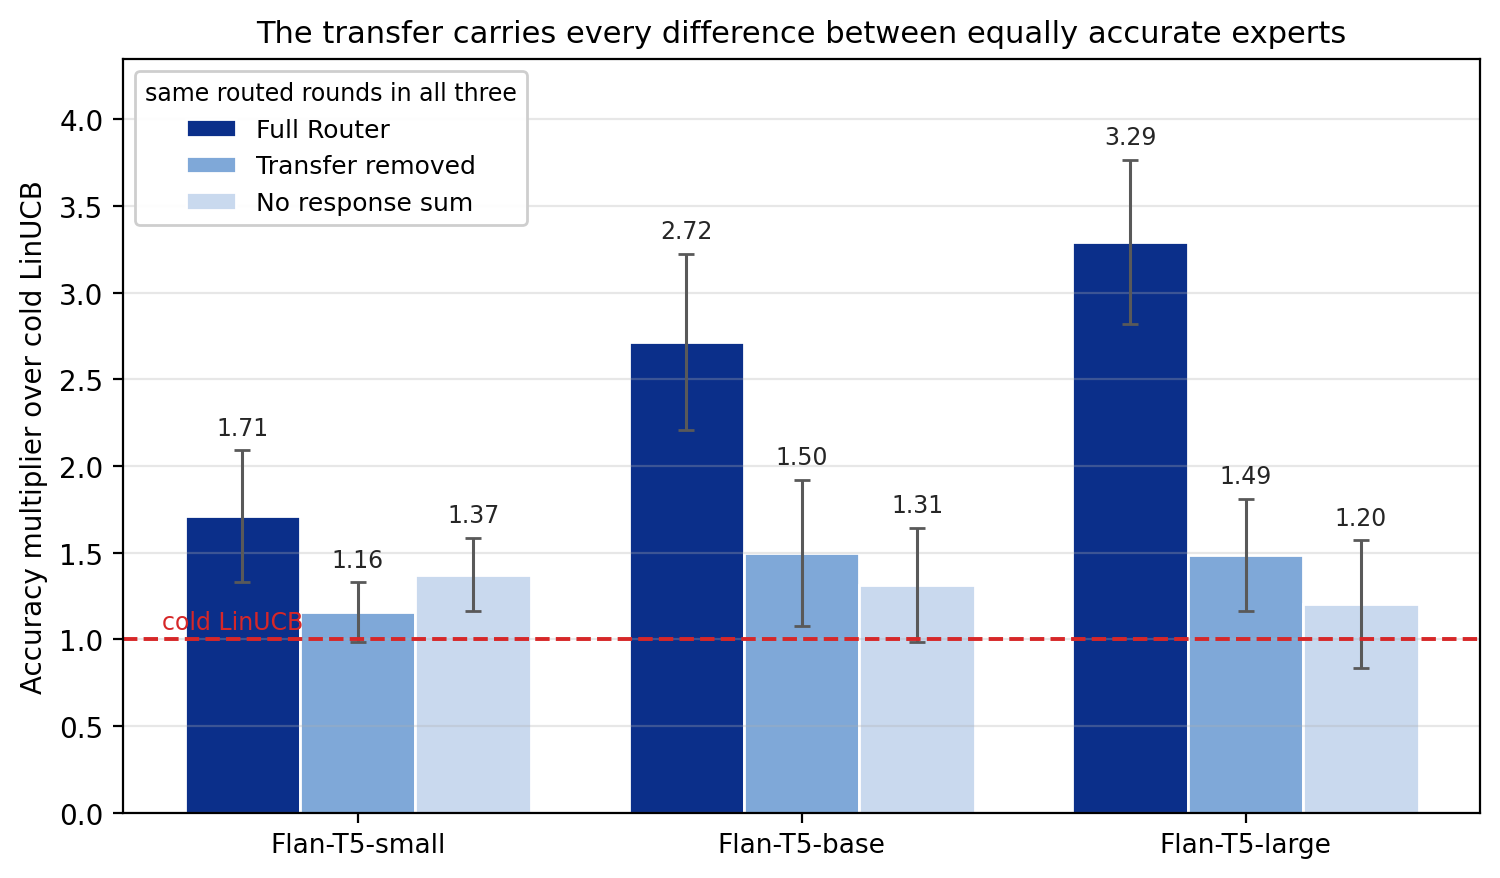
\includegraphics[width=0.68\linewidth]{two_channel.png}
\caption{\rev{Coverage versus the transfer: accuracy multiplier over cold LinUCB
(ten seeds, standard errors). All versions route the rounds the full Router
chose. \emph{Transfer removed} feeds the prediction
$\langle\theta_{\mathrm{or}},\phi\rangle$ of a ridge fit on held-out data
instead of the reward on those rounds, and \emph{no response sum} feeds
nothing. Without the transfer, the experts are indistinguishable.}}
\label{fig:two-channel}
\end{figure}

\begin{revised}
The results support (P1) and (P2). The three experts' held-out accuracies
order them differently from their accuracy multipliers
(Table~\ref{tab:amazon-results}). Almost all of each Router's advantage, $96$
to $100\%$, is tail value $I_\tau$, earned after the routed rounds
(Table~\ref{tab:amazon-decomp}). The experts cover the directions on which
cold LinUCB is trapped to within $5\%$, at nearly the same prices
(Appendix~\ref{app:amazon-transfer}). To test whether the transfer carries
the difference, we replay each run with the routed rounds held fixed, so
that every version of the learner has the same coverage
(Figure~\ref{fig:two-channel}). On the routed rounds we feed the learner
$\langle\theta_{\mathrm{or}},\phi\rangle$ instead of the observed reward,
where $\theta_{\mathrm{or}}$ is a ridge-regression fit of the reward on
held-out data. This deletes the transfer~\eqref{eq:transfer} with
$\theta^\star=\theta_{\mathrm{or}}$, and it turns every significant pairwise
difference between experts into a null result. For example, the paired
$t$-statistic of the large expert over the small one drops from $5.18$ to
$1.33$. Coverage alone saves $2$ to $3.5\%$ of cold LinUCB's regret for every
expert, while the full Router saves $6.5\%$, $16\%$ and $21\%$.
\end{revised}

\begin{figure}[t]
\centering
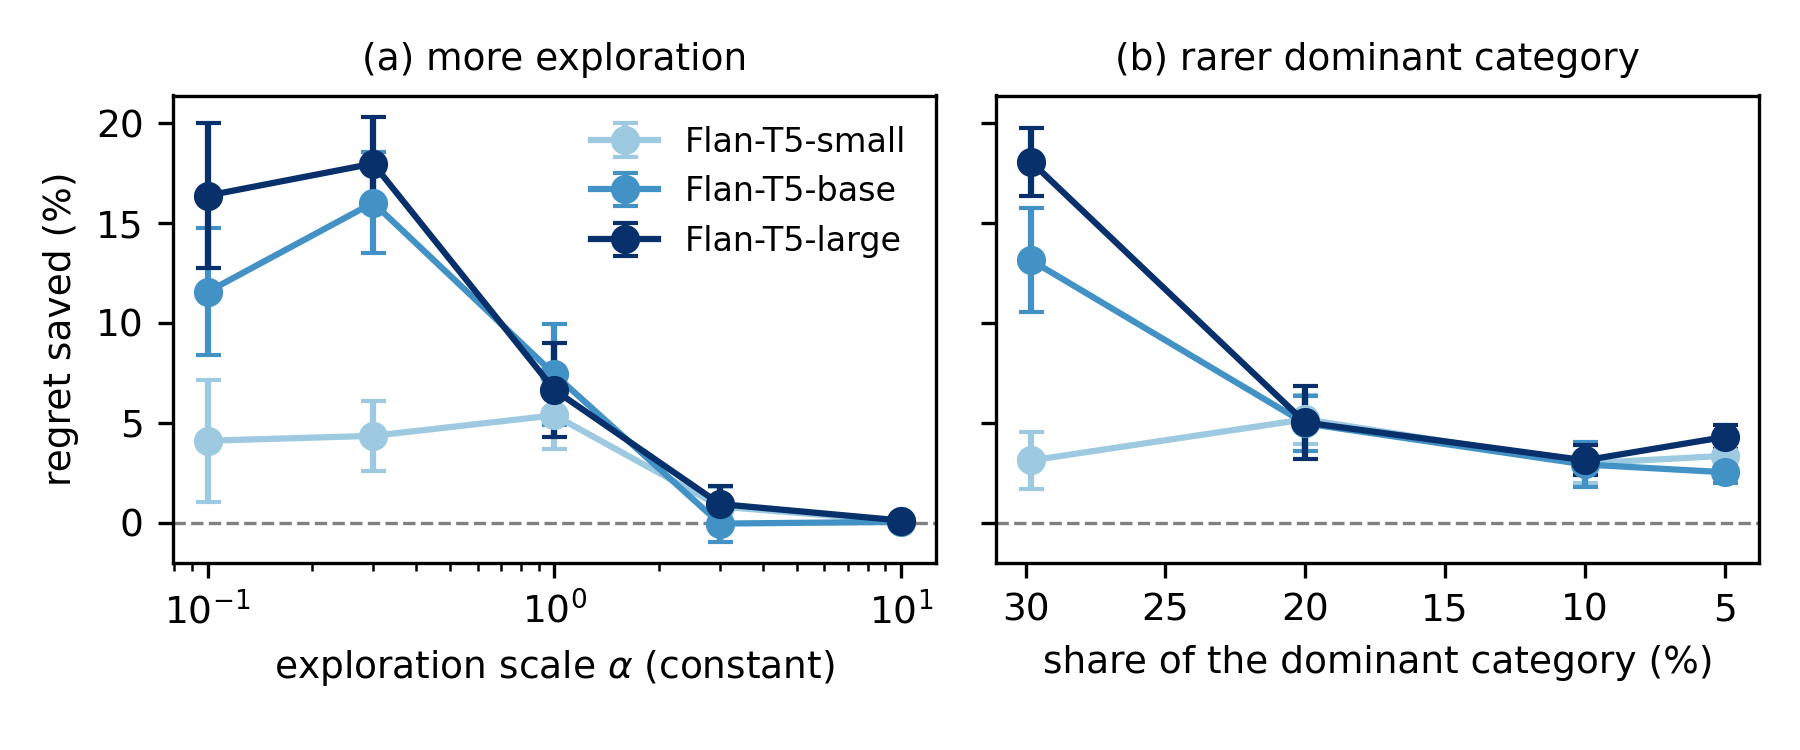
\includegraphics[width=0.9\linewidth]{regimes.png}
\caption{The two regimes: share of cold LinUCB's regret the Router saves
(seeds $1$--$10$, bootstrap errors). (a) A constant exploration scale
$\alpha$ for both policies. (b) Every category's share of contexts capped
\rev{($29.8\%$ is the natural share), on streams of $14{,}000$ rounds. The
numbers are in Appendix~\ref{app:main-details}.}}
\label{fig:regimes}
\label{fig:exploration}
\label{fig:skew}
\end{figure}

\begin{revised}
The data also support (P3). LinUCB tends to settle on one frequent category
and then predicts it on a large share of rounds. Runs that settle on the
dominant category finish near $28\%$ accuracy, and cold LinUCB does so in
$1$ of $20$ seeds. Whether a Router settles there is decided by a handful of
routed answers. Across $177$ Router runs, a run whose expert gave no correct
routed answer on this category reached it in $3$ of $45$ runs, and a run
whose expert gave five or more did so in all $54$ (Table~\ref{tab:dose}).
This is the mechanism of Theorem~\ref{thm:transfer-separation}. The dominant
category plays the role of $D$, the thousands of categories that cold
LinUCB keeps trying play the fresh arms, and the product text, which the LLM
reads and LinUCB sees only through its features, plays the hidden type
(Remark~\ref{rem:transfer-amazon}). The match is qualitative. No run meets
the sufficient condition of Theorem~\ref{thm:settling} at the handoff, and
LinUCB's own plays complete the settling after routing has mostly stopped
(Appendix~\ref{app:settling-data}). As part~(ii) of
Theorem~\ref{thm:settling} predicts, coverage without rewards buys nothing.
Adding $75$ correct answers on the dominant category to Flan-T5-small raises
its accuracy multiplier from $1.71\times$ to $2.56\times$ ($p=0.007$). The
same answers with their rewards hidden give $1.84\times$ ($p=0.61$), as do
correct answers on random categories (Table~\ref{tab:inject50k}). An expert
should therefore be chosen by where its correct answers fall, and not by its
accuracy. Appendix~\ref{app:diagnostics} gives a held-out dry run that makes
this choice before deployment.
\end{revised}

\begin{revised}
Finally, the gain behaves as (P4) predicts. Raising the exploration scale,
held constant for both policies, from $\alpha\le0.3$ to $\alpha=3$ takes
the saving of the two larger experts from $12$--$18\%$ of cold LinUCB's
regret to under $1\%$ (Figure~\ref{fig:regimes}a). As exploration approaches
what the theory asks for, the learner stops settling. Capping the dominant
category's share at $20\%$ or below takes their saving from $13$--$18\%$ to
$2.5$--$5\%$, the size of the coverage-only gain
(Figure~\ref{fig:regimes}b). WikiLinks, where no entity covers more than
$0.36\%$ of contexts, is the far end of the same curve, with accuracy
multipliers of $0.93\times$ to $1.05\times$.
\end{revised}

\begin{revised}
The gains survive stronger baselines. Tuned on held-out seeds, cold LinUCB
is no better, and the Router still multiplies its accuracy by $2.07$ to
$3.03$ (Table~\ref{tab:amazon-results}). Adding the category embedding to
the features, $\phi(x,a)=[x\odot z_a,z_a]$, lets cold LinUCB learn how often
each category is right, yet it helps the Router more, which then saves $20$
to $34\%$ of cold LinUCB's regret. With BGE features and Qwen2.5 experts,
cold LinUCB is much stronger, yet two of the three experts still cut its
regret by about $14\%$, again not in order of accuracy
(Appendix~\ref{app:bge}). Neither CORRAL nor offline warm starts are
significantly better than the Router (Appendix~\ref{app:routers}).
\end{revised}

\section{Conclusion}
\label{sec:conclusion}

\begin{revised}
We studied why a fixed LLM expert followed by LinUCB can beat both, and why
the expert's accuracy does not predict the gain. The expert's data reaches
the learner through coverage and through the transfer. With the exploration
that LinUCB's theory requires, we proved that coverage helps only as far as
a ratio of prices allows, and that under linear rewards it is all the data
provides. With the reduced exploration used in practice, we proved that the
transfer decides whether LinUCB settles on an action. It can then separate
experts with identical coverage, cost and number of correct answers by a
factor of order the horizon. On AmazonCat-13K, the transfer carries every
significant difference between experts. Our main conclusion is that an
expert's value to the learner is decided by where its correct answers fall.
An expert should therefore be chosen by where it is right, and not by how
often.
\end{revised}

\begin{revised}
\paragraph{Limitations and future work.}
Our price bound assumes linear rewards and a fixed set of arms that always
contains a best arm. AmazonCat lies outside this setting, so on that dataset
the bound explains why coverage cannot account for the gains but does not
predict their size. Extending the price analysis to misspecified rewards and
changing action sets would close this gap. Our results on the transfer
require exploration below a valid radius. This is the regime of practice,
but LinUCB's regret guarantees do not hold there. A theory that gives both
settling and a regret guarantee, for example with a radius that adapts to
the data, is an open direction. Our settling theorems describe the mechanism
on AmazonCat but do not certify it. On the logged runs the margin is
negative at the handoff, and LinUCB's own later plays complete the settling.
A theory of margins that build up after the handoff, together with
measurements of the quantities of Appendix~\ref{app:settling-context} on the
logged runs, would address this. Our constructions use constant radii,
unoptimized constants and large instances, and the Router result needs
$q<\omega$. Constructions with decaying radii and smaller instances would
show how general the effect is. Finally, the large gains appear in one
configuration and depend on a dominant category, whose frequency we vary
only by subsampling AmazonCat. Testing the predictions on datasets whose
label frequencies differ naturally is the most direct next step.
\end{revised}

\acks{We thank ...}

\bibliography{references}


\appendix

\section{Related Work}\label{sec:related}
\begin{revised}
This appendix extends the comparison of Section~\ref{sec:intro}. We group
the work closest to ours by the problem it addresses and say how our results
differ.

\paragraph{Combining LLMs with contextual bandits.}
\citet{chen2024llmdecision} combine an LLM policy with a contextual bandit
learner through an online model-selection master and document reward
multiplication on large recommendation datasets. Our
experiments follow their setup. We give an account of where the gain comes
from, and we use a deterministic confidence-gated rule in place of their
randomized master. \citet{huangcontextual} calibrate an embedding-based
estimate of the LLM's uncertainty and use it to adjust UCB-style exploration
bonuses. They bound the regret of a single calibrated agent through the
accuracy of the LLM's reward predictions. We decompose the hybrid's
advantage exactly, cap what coverage can buy by a ratio of prices, and show
that under reduced exploration the value of an expert's data is decided by
where its rewarded answers fall, which accuracy does not capture.
\citet{jumpstart2026} warm-start a linear bandit from LLM-generated
preferences. They bound the error of the warm-started estimate through a
single prior-error term measured in the geometry of the pretraining design
matrix, and they treat the design matrix and the response vector as one
object. We separate the two, show that under linear rewards the second is
determined by the first (Observation~\ref{prop:response-sum}), and identify
the expert-dependent remainder, the transfer, in closed form.
\citet{calibgated2026} inject LLM pseudo-observations into LinUCB with a
weight that depends on calibration, on both the design matrix and the
response vector. Their rule is close in spirit to ours, and they analyze it
through a bias--variance argument without a regret bound. Our decomposition
and price bound apply to any such rule. Work on LLMs as exploring agents
shows that LLMs can learn in context to explore
\citep{monea2024llms,krishnamurthy2024can} and that LLM-derived priors can
speed up exploration \citep{alamdari2024jumpstarting,abbasiyadkori2024believe}.
These works study the LLM as the learner. We keep the LLM fixed and study
what its data does to a separate learner.

\paragraph{Warm starts, offline data and hints.}
Initialization from logged data, offline data and pretrained predictors can
improve a contextual bandit's early performance
\citep{zhang2019warm,riquelme2018deep}, as can transfer and meta-learning
across tasks \citep{lazaric2012transfer,gentile2014online,sharaf2019meta}.
Hybrid and offline-to-online reinforcement learning
\citep{song2022hybrid,wagenmaker2023leveraging,hao2023leveraging} likewise
bounds the benefit of offline data through its coverage. These analyses
value the data by its quality or coverage and do not charge for acquiring
it. We charge for it, and the acquisition can exceed the data's value.
\citet{bastani2021mostly} show that a greedy learner can do well without
exploration under diverse contexts, and that an under-exploring learner can
lock onto whatever paid first. We show that, for an online warm start, this
lock-in makes the value of an expert's data depend on where its correct
answers fall. The price of Section~\ref{sec:price} is the single-direction
counterpart of the allocation programs behind asymptotic instance-dependent
lower bounds, in which regret is minimized subject to coverage constraints
on every direction \citep{graves1997asymptotically,lattimore2017end}. Our
use of it is non-asymptotic and comparative. Closest among analyses of side
information is \citet{cutkosky2022leveraging}, where the learner receives a
hint about $\theta^\star$ and the regret improves with the hint's accuracy
\citep[see also][]{rakhlin2013online}. Our warm start is data, not a hint,
and its value is not a function of accuracy:
Theorem~\ref{thm:transfer-separation} gives two experts of equal coverage,
cost and number of correct answers whose values differ by a factor of order
the horizon.

\paragraph{Model selection and expert aggregation.}
Expert-learning methods compete with the best fixed expert in hindsight
\citep{auer2002nonstochastic}. In bandits, CORRAL
\citep{agarwal2017corralling} combines base algorithms through online mirror
descent with a log-barrier regularizer and competes with the best of them,
and later work tightens the rates and extends the framework
\citep{pacchiano2020model,marinov2021pareto,zhu2022pareto,zhu2022near,dann2024data}.
These masters are randomized and target robustness, doing nearly as well as
the best base algorithm, whichever it is. We determine instead when a
combination beats all of its components. The decomposition of
Proposition~\ref{prop:decomp} and the price bound of
Theorem~\ref{thm:general-price} hold for any routed set, so they apply to
CORRAL as to our deterministic Router.

\paragraph{Misspecified linear bandits.}
Work on misspecified linear bandits
\citep{ghosh2017misspecified,lattimore2020learning,foster2020adapting}
bounds the extra regret caused by the part of the reward that the linear
model misses. In our setting that part, carried by the transfer, is the main
source of the gain.
\end{revised}

\section{The Price Bound in Full}
\label{app:moved}

This appendix states the general form of Theorem~\ref{thm:general-price},
of which the main text gives the case in which every suboptimal arm is
certified and no coverage comes free from optimal arms.

\paragraph{No free coverage.}
\begin{lemma}[No free coverage]
\label{lem:no-free-coverage}
For any policy $\pi$, any interval $I$ of rounds, and any direction $u$,
$\sum_{t\in I}\langle x_{t,\pi_t},u\rangle^2\le R_I(\pi)/\kappa(u)$.
Consequently, if $\Hyb_\tau$ hands off with design matrix $V_{\tau+1}=\lambda I+M_\tau$, then
for every unit vector $u$,
$\|u\|^2_{V_{\tau+1}^{-1}}\ \ge\ 1\big/\bigl(\lambda+R_{[1,\tau]}(\Exp)/\kappa(u)\bigr)$.
\end{lemma}

The lemma is proved in Appendix~\ref{app:catalog}.

\paragraph{Setting.}
In words: we fix a finite set of arms in which the best arm is always
offered, compare cold LinUCB with an arbitrary policy $\pi$ up to a cutoff
$t_0$, and measure how much coverage $\pi$ bought, at what price, and which
arms that coverage lets the confidence bound rule out. Let
$\mathcal X\subset\R^d$ be a finite set of arm vectors with $\|x\|_2\le L$,
let $\mathcal A_t\subseteq\mathcal X$ for every $t$, and suppose an arm
$x^\star$ with $\mu(x^\star)=\max_{x\in\mathcal X}\mu(x)$ belongs to every
$\mathcal A_t$. The gap of an arm is then the same at every round,
$\Delta(x):=\mu(x^\star)-\mu(x)$; write $\mathcal S:=\{x\in\mathcal X:\Delta(x)>0\}$
and fix $\beta\ge\beta_t$ for every $t\le T$ (one exists because
$\|x\|_2\le L$ bounds $\det V_t$).

\emph{What cold LinUCB pays.} For $x\in\mathcal S$ put $u_x:=x/\|x\|_2$ and
\begin{gather*}
\kappa_x:=\frac{\Delta(x)}{\|x\|_2^2},\qquad
C^\star_x:=\frac{4\beta^2\|x\|_2^2}{\Delta(x)^2},\\
n^\star_x:=\Bigl(\frac{C^\star_x-\lambda}{\|x\|_2^2}+1\Bigr)\ind\{C^\star_x\ge\lambda\},\qquad
N_x:=\#\{t\in[T]:x\in\mathcal A_t\}.
\end{gather*}
Here $\kappa_x$ is the price of covering $u_x$ by pulling $x$ itself,
$C^\star_x-\lambda$ is the least coverage of $u_x$ at which the confidence
bound can exclude $x$, and $n^\star_x$ bounds how often cold LinUCB pulls $x$
before its own pulls exclude it.

\emph{What $\pi$ pays.} Write $x^\pi_t$ for the arm $\pi$ plays at round $t$
and, for a set $U\subseteq\mathcal S$ of arms,
$\mathrm{cov}_U(x):=\sum_{y\in U}\langle x,u_y\rangle^2$. The price $\pi$ pays
for coverage of $U$ up to $t_0$, and the coverage of $U$ it obtains for free
by playing optimal arms, are
\begin{gather*}
\kappa^\pi_U(t_0):=\min\Bigl\{\frac{\Delta(x^\pi_t)}{\mathrm{cov}_U(x^\pi_t)}:
\ t\le t_0,\ \Delta(x^\pi_t)>0,\ \mathrm{cov}_U(x^\pi_t)>0\Bigr\},
\\
C^{\mathrm{free}}_U(t_0):=\sum_{t\le t_0:\,\Delta(x^\pi_t)=0}\mathrm{cov}_U(x^\pi_t),
\end{gather*}
with the minimum over an empty set equal to $+\infty$. Finally
$U_{\mathrm{cert}}(t_0)$ is the set of arms $x\in\mathcal S$ that $\pi$'s
first $t_0$ rounds certify: $2\beta\|x\|_{(V^\pi_{t_0+1})^{-1}}<\Delta(x)$, with
$V^\pi_{t_0+1}=\lambda I+\sum_{t\le t_0}x^\pi_t (x^\pi_t)^\top$. For the
handoff hybrid with $t_0=\tau$, $\kappa^\pi_U(\tau)$ is the expert's price and
$R_{[1,t_0]}(\pi)$ its acquisition regret, but nothing below uses this.

\begin{theorem}[Price bound, general form]
\label{thm:general-price-full}
In the setting above, on the confidence event of cold LinUCB, let $\pi$ be
any policy, $t_0\in\{0,\dots,T\}$ any cutoff and $U\subseteq
U_{\mathrm{cert}}(t_0)$ any set of certified arms, and write
$\kappa^{\Cold}_U:=\max_{x\in U}\kappa_x$ ($:=0$ if $U=\emptyset$) and
$P_U:=\kappa^{\Cold}_U/\kappa^\pi_U(t_0)$ for the price ratio. Then
\[
R_T(\Cold)\ \le\ P_U\,R_{[1,t_0]}(\pi)\ +\ \kappa^{\Cold}_U\,C^{\mathrm{free}}_U(t_0)\ +\ \sum_{x\in U}\Delta(x)
\ +\sum_{x\in \mathcal S\setminus U}\Delta(x)\min\{n^\star_x,N_x\},
\]
and consequently, whenever $R_T(\pi)>0$,
\begin{equation}
\label{eq:general-price}
\frac{R_T(\Cold)}{R_T(\pi)}\ \le\ P_U\ +\
\frac{\kappa^{\Cold}_U\,C^{\mathrm{free}}_U(t_0)+\sum_{x\in U}\Delta(x)+\sum_{x\in \mathcal S\setminus U}\Delta(x)\min\{n^\star_x,N_x\}}{R_T(\pi)} .
\end{equation}
For $\pi=\Hyb_\tau$ and $t_0=\tau$ this bounds the regret ratio of the
hybrid by the price ratio between cold exploration and the expert on the
arms the warm start certifies, plus a residual.
\end{theorem}


Theorem~\ref{thm:general-price} is the case $U=\mathcal S$: then
$\kappa^{\Cold}_U=\max_{x\in\mathcal S}\kappa_x$, $\kappa^\pi_U(t_0)=\kappa^\pi(t_0)$,
$C^{\mathrm{free}}_U(t_0)=0$ when the optimal arms $\pi$ plays are orthogonal
to $\mathcal S$, and the last sum is empty.

\emph{What the bound says.} The proof (Appendix~\ref{app:proof-general-price})
has two steps: cold LinUCB pays its own price once per arm, since its own
pulls of an arm shrink that arm's width below its gap; and any policy that
certifies an arm must buy the same coverage, at no less than its own price
per unit. Only cold LinUCB's confidence event is used and $\pi$ is
arbitrary, so the bound covers the fixed-$\tau$ hybrid, the adaptive Router
and a CORRAL-style master alike. The price ratio covers the arms the policy
paid to certify; the residual is what nobody paid for, chiefly cold LinUCB's
regret on the arms the warm start does not certify. The theorem therefore
caps the \emph{certified saving} rather than the regret ratio outright, and
because the residual is counted arm by arm it can be loose when many arms
share directions. Whether the residual can be large without a large price
ratio is open. The bound holds whether the saving is collected during the
routed rounds ($A_\tau$) or after them ($I_\tau$), and the confidence radius
cancels in $P_U$ because it scales $C^\star_x$, the coverage both policies
must reach, identically.

\section{Tools: the Decomposition and the Widths}
\label{app:extra-theory}

This appendix collects the tools used in the main text: the decomposition
holds pathwise and for any routed set, LinUCB's regret on a round is limited
by the widths of its competitors, and a warm start shrinks widths only in the
directions it covers.

\subsection{The Identity in General, and Width-Limited Regret}
\label{app:width-limited}
\label{sec:width}

\begin{remark}
\label{rem:decomp}
The identities hold pathwise in the reward-table model, in which the $k$-th
pull of an action always receives the same noise draw, so that two policies
can be run on the same noise \citep[\S4.6]{lattimore2020bandit}, and
therefore also in expectation. They also hold when the routed rounds are not
an initial segment: for any set $\mathcal T\subseteq[T]$ of routed rounds,
fixed in advance or chosen adaptively (as by the Router of
Appendix~\ref{app:meta-algorithm}), replacing $[1,\tau]$ by $\mathcal T$
gives the same identities, because each side is a difference of sums over a
partition of $[T]$. If the warm start $(M,c)$ is built from data outside the
horizon (an \emph{offline} warm start $\Hyb^{\mathrm{off}}$, LinUCB started
from $(\lambda I+M,c)$), the routed rounds are not charged and the identities
read $R_T(\Cold)-R_T(\Hyb^{\mathrm{off}})=:I^{\mathrm{off}}$ and
$R_T(\Exp)-R_T(\Hyb^{\mathrm{off}})=:B^{\mathrm{off}}$. A large regret ratio over both
base policies means that $A_\tau+I_\tau$ is almost all of $R_T(\Cold)$ and
$B_\tau$ almost all of $R_T(\Exp)$; every diverging ratio in this paper is
read along a sequence of instances.
\end{remark}

Fix the confidence event $\mathcal E_\delta$ on which
$\|\widehat\theta_t-\theta^\star\|_{V_t}\le\beta_t$ for all rounds $t$ at
which LinUCB acts, where $(V_t,c_t)$ are built from all data so far including
any warm start $(M,c)$ formed from the same kind of data; by the
self-normalized bound of \citet{abbasi2011improved} this event has probability
at least $1-\delta$ with
$\beta_t=\sigma\sqrt{2\log(\det(V_t)^{1/2}\det(\lambda I)^{-1/2}/\delta)}+\sqrt\lambda S$.
Define, for a positive definite $V$,
\begin{equation}
\label{eq:phi}
\Phi_t(V)\;:=\;\max_{a\in\mathcal A_t}\;\min\Bigl\{\Delta_{t,a},\;2\beta_t\|x_{t,a}\|_{V^{-1}}\Bigr\}.
\end{equation}

\begin{lemma}[Width-limited regret]
\label{lem:width-limited}
On $\mathcal E_\delta$, at any round $t$ at which LinUCB acts with design
matrix $V_t$, the instantaneous pseudo-regret satisfies
$\Delta_{t,A_t}\le\Phi_t(V_t)$. Moreover $\Phi_t$ is monotone: $V\preceq V'$
implies $\Phi_t(V')\le\Phi_t(V)$ when the radius $\beta_t$ is held fixed.
\end{lemma}

\subsection{How Widths Shrink}
\label{app:widths}

\begin{lemma}[A warm start shrinks widths in the directions it covers]
\label{lem:loewner}
For any $M\succeq0$ and any $x$, $\|x\|_{(\lambda I+M)^{-1}}\le\|x\|_{(\lambda I)^{-1}}=\|x\|_2/\sqrt\lambda$.
If $P$ is an orthogonal projector, $M\succeq mP$, and $x\in\mathrm{Im}(P)$, then
$\|x\|^2_{(\lambda I+M)^{-1}}\le\|x\|_2^2/(\lambda+m)$. If instead $x\perp\mathrm{Im}(M)$,
then $\|x\|_{(\lambda I+M)^{-1}}=\|x\|_2/\sqrt\lambda$: a warm start does nothing
for directions it does not cover.
\end{lemma}

\section{The Price Ratio Attained}
\label{app:catalog-statements}

This appendix states Theorem~\ref{thm:price}, which shows that the price
bound is attained up to a constant factor. The instance is defined in
Appendix~\ref{app:template-thm} below, after the conventions it uses; the
proof is in Appendix~\ref{app:catalog}.

\subsection{Standing Conventions}
\label{sec:template}

Noise is i.i.d.\ $\sigma$-sub-Gaussian and independent of the actions; we use
the reward-table model in which the $m$-th pull of a given action vector
receives the $m$-th entry of an i.i.d.\ sequence attached to that vector
\citep[\S4.6]{lattimore2020bandit}, which has the same law as the sequential
model and lets us compare two policies on the same noise. We fix
\begin{equation}
\label{eq:conventions}
L\ge8,\quad \gamma\in(0,1],\quad 0<\eps<\gamma/L,\quad
\lambda\ \ge\ \max\bigl\{\sigma^2d\,\ell_0,\ 8\sigma^2\ell_1,\ 60\bigr\},\quad
\beta\equiv2\sqrt\lambda,
\end{equation}
with $\ell_0:=\log(1+TL^2)+2\log(1/\delta)$ and $\ell_1:=\log(2dT/\delta)$.
The confidence radius is constant. The lower bound on $\lambda$ makes
$2\sqrt\lambda$ at least the radius of \citet{abbasi2011improved} at every
round, so the confidence event of Section~\ref{sec:width} holds for each
policy with probability $\ge1-\delta$, and it makes the noise on any $\lambda/30$
pulls of one arm smaller than a quarter of that arm's confidence bonus. The
constant $m_0:=\lfloor\lambda/30\rfloor\ge2$ is the number of pulls of a
fresh bad arm that optimism forces before the good arm or the probe can be
preferred to it. Conditions on $T$ appear in each statement; they only say
that the horizon is long enough for the claimed rounds to take place.


\subsection{The Template, and the Price Ratio Attained}
\label{app:template-thm}

The instance has a good arm, bad arms along $K$ recurring orthogonal
directions, and a cheap informative action, the \emph{probe}, that is offered
only during a window. Fix $K\ge1$ and set $d=K+1$. The parameter is $\theta^\star=e_1$. Directions
cycle: $j(t):=2+((t-1)\bmod K)$. Three actions may be offered at round $t$:
\[
g:=e_1\ (\mu=1),\qquad
b_t:=Le_{j(t)}\ (\mu=0),\qquad
p_t:=(1-\eps)e_1+\gamma\,e_{j(t)}\ (\mu=1-\eps),
\]
the \emph{good} arm, the \emph{bad} arm, and the \emph{probe}. The instance
$\mathcal I(K,L,\gamma,\eps,\tau_0)$ has $\mathcal A_t=\{g,b_t,p_t\}$ for $t\le\tau_0$
and $\mathcal A_t=\{g,b_t\}$ for $t>\tau_0$. The price of $e_j$, $j\ge2$, is
$\min\{1/L^2,\eps/\gamma^2\}$ while probes are offered and $1/L^2$ afterwards. The
expert is the frozen linear policy $\Exp_w$ that plays
$\arg\max_{a\in\mathcal A_t}\langle\widehat\theta_{\Exp},x_{t,a}\rangle$ with
$\widehat\theta_{\Exp}=e_1+w\sum_{j\ge2}e_j$; ties do not occur for the values
of $w$ we use. Throughout, $\tau_0=Kn$ for an integer $n$, so each direction is
probed exactly $n$ times by a policy that plays every probe.

We work under the standing conventions \eqref{eq:conventions} of
Appendix~\ref{sec:template}: $L\ge8$, $\gamma\in(0,1]$, $0<\eps<\gamma/L$,
$\lambda\ge\max\{\sigma^2d\,\ell_0,8\sigma^2\ell_1,60\}$ with $\ell_0,\ell_1$
logarithmic in $T/\delta$, and the constant radius $\beta=2\sqrt\lambda$, in
the reward-table noise model of Remark~\ref{rem:decomp}; we write
$m_0:=\lfloor\lambda/30\rfloor$ for the number of pulls of a fresh bad arm
that optimism forces.

On $\mathcal I(K,L,\gamma,\eps,\tau_0)$ the expert $\Exp_w$ with
$w\in(1/L,(1-\eps)/(L-\gamma))$ plays every probe while probes are offered and
every bad arm afterwards (Lemma~\ref{lem:expert-routes}). Its routed actions
cost $\eps$ each, cover $e_{j(t)}$ at rate $\gamma^2$ per round, and recur; after
$\tau_0$ it is the worst possible policy. The hybrid that hands off exactly
when the probes disappear therefore isolates the price ratio.

\begin{theorem}[The price ratio attained as the regret ratio]
\label{thm:price}
Let $\mathcal I=\mathcal I(K,L,\gamma,\eps,Kn)$ under \eqref{eq:conventions}, with
$\Exp=\Exp_w$ for some $w\in(1/L,(1-\eps)/(L-\gamma))$, and $\tau=\tau_0=Kn$. With
probability at least $1-3\delta$ the following hold simultaneously.
\begin{enumerate}[itemsep=1pt,topsep=1pt,leftmargin=*]
\item[(i)] \emph{(Expert.)} $R_T(\Exp)=\eps Kn+(T-Kn)$.
\item[(ii)] \emph{(Cold, lower bound.)} If $n\ge m_0$ then
$R_{[1,Kn]}(\Cold)\ge Km_0$; in particular $A_{\tau_0}\ge Km_0-\eps Kn$.
\item[(iii)] \emph{(Cold, upper bound.)} For every $n\ge1$, $R_T(\Cold)\le K(8\beta^2+1)+\eps Kn$.
\item[(iv)] \emph{(Hybrid.)} If $n\ge36\lambda L^2/\gamma^2$ and $K\ge36L^2$, then
$\Hyb_{\tau_0}$ plays $g$ at every round $t>\tau_0$, so
$R_T(\Hyb_{\tau_0})=\eps Kn$, $I_{\tau_0}=R_{[Kn+1,T]}(\Cold)\ge0$, and
$B_{\tau_0}=T-Kn$.
\end{enumerate}
Consequently, for $n\ge36\lambda L^2/\gamma^2$ and $K\ge36L^2$,
\begin{equation}
\label{eq:price-ratio}
\frac{m_0}{\eps n}\ \le\ \frac{R_T(\Cold)}{R_T(\Hyb_{\tau_0})}\ \le\ 1+\frac{8\beta^2+1}{\eps n},
\qquad
\frac{R_T(\Exp)}{R_T(\Hyb_{\tau_0})}=1+\frac{T-Kn}{\eps Kn},
\end{equation}
and at the smallest admissible $n=\lceil36\lambda L^2/\gamma^2\rceil$ the first
ratio is $\Theta(\gamma^2/(\eps L^2))$, with explicit constants
$\gamma^2/(2220\,\eps L^2)\le R_T(\Cold)/R_T(\Hyb_{\tau_0})\le1+\gamma^2/(\eps L^2)$
(the constants of this section are not optimized; see
Appendix~\ref{app:catalog}, ``Remarks on the constants'').
\end{theorem}

The bracket \eqref{eq:price-ratio} is the price ratio: cold exploration buys
coverage $L^2$ of a bad direction per unit of regret (price $1/L^2$), the
probe buys $\gamma^2$ per $\eps$ (price $\eps/\gamma^2$), and the regret ratio over cold
LinUCB is their ratio $\gamma^2/(\eps L^2)$ up to constants. The conditions on
$n$ and $K$ in (iv) are not about prices alone. Enough coverage of $e_j$ is
necessary for the handoff matrix to certify $b_j$ but not sufficient: every
probe is orthogonal to $v=\gamma\,e_1-(1-\eps)\sum_{j\ge2}e_j$, so the width of
$e_j$ stays at least $(1-\eps)/\sqrt{\lambda(\gamma^2+K(1-\eps)^2)}$ however many
probes are played, and certification needs $K$ of order $L^2$; the price
ratio does not see this geometric condition. The instances are large by
design: orthogonal bad directions stand in for an action space too large for
cold exploration to exhaust (AmazonCat has $13{,}330$ categories), and at the
smallest admissible sizes the window alone exceeds $3\times10^8$ rounds. The regret ratio over
the expert, $(T-\tau_0)/(\eps\tau_0)$, diverges as the tail lengthens. Here
the saving is collected during the routed rounds, as $A_{\tau_0}$.

\section{Proofs}
\label{app:proofs}

This appendix proves the decomposition identity, the width lemmas of
Appendix~\ref{app:extra-theory}, Observation~\ref{prop:response-sum} and
Theorem~\ref{thm:general-price-full}.

\subsection{Proof of Proposition~\ref{prop:decomp}}
\label{app:proof-decomp}

\begin{proof}
Split $[T]$ into $[1,\tau]$ and $[\tau+1,T]$. On $[1,\tau]$ the hybrid plays
$a_t^{\Exp}$, so $R_{[1,\tau]}(\Hyb_\tau)=R_{[1,\tau]}(\Exp)$. Hence
\[
R_T(\Cold)-R_T(\Hyb_\tau)
=\bigl(R_{[1,\tau]}(\Cold)-R_{[1,\tau]}(\Exp)\bigr)
+\bigl(R_{[\tau+1,T]}(\Cold)-R_{[\tau+1,T]}(\Hyb_\tau)\bigr)
=A_\tau+I_\tau ,
\]
and
\[
R_T(\Exp)-R_T(\Hyb_\tau)
=\bigl(R_{[1,\tau]}(\Exp)-R_{[1,\tau]}(\Exp)\bigr)
+\bigl(R_{[\tau+1,T]}(\Exp)-R_{[\tau+1,T]}(\Hyb_\tau)\bigr)
=B_\tau .
\]
Both are identities between sums of gaps, so they hold for every noise
realization and therefore in expectation.
\end{proof}

\subsection{Proof of Lemma~\ref{lem:width-limited}}
\label{app:proof-width}

\begin{proof}
Fix a round $t$ at which LinUCB acts, and write $x^\star=x_{t,a_t^\star}$,
$x=x_{t,A_t}$, $\wid(u)=\|u\|_{V_t^{-1}}$. On $\mathcal E_\delta$, Cauchy--Schwarz
gives $|\langle\widehat\theta_t-\theta^\star,u\rangle|\le\beta_t\wid(u)$ for
every $u$. By the selection rule,
$\langle\widehat\theta_t,x\rangle+\beta_t\wid(x)\ge\langle\widehat\theta_t,x^\star\rangle+\beta_t\wid(x^\star)\ge\langle\theta^\star,x^\star\rangle$,
and $\langle\widehat\theta_t,x\rangle\le\langle\theta^\star,x\rangle+\beta_t\wid(x)$.
Combining, $\Delta_{t,A_t}=\langle\theta^\star,x^\star-x\rangle\le2\beta_t\wid(x)$.
Thus $\Delta_{t,A_t}=\min\{\Delta_{t,A_t},2\beta_t\wid(x_{t,A_t})\}\le\max_a\min\{\Delta_{t,a},2\beta_t\wid(x_{t,a})\}=\Phi_t(V_t)$.
Monotonicity: $V\preceq V'$ implies $V'^{-1}\preceq V^{-1}$, so every width is
non-increasing and so is each term in the maximum.
\end{proof}

\subsection{Proof of Lemma~\ref{lem:loewner}}
\label{app:proof-loewner}

\begin{proof}
$\lambda I+M\succeq\lambda I$ gives $(\lambda I+M)^{-1}\preceq(\lambda I)^{-1}$,
which is the first claim. For the second, $\lambda I+M\succeq\lambda I+mP$, so
$x^\top(\lambda I+M)^{-1}x\le x^\top(\lambda I+mP)^{-1}x$, and for
$x\in\mathrm{Im}(P)$ the right-hand side is $\|x\|_2^2/(\lambda+m)$ because
$(\lambda I+mP)^{-1}$ acts as $(\lambda+m)^{-1}$ on $\mathrm{Im}(P)$. For the
third, if $x\perp\mathrm{Im}(M)$ then $x$ is an eigenvector of $\lambda I+M$
with eigenvalue $\lambda$, so $x^\top(\lambda I+M)^{-1}x=\|x\|_2^2/\lambda$.
\end{proof}

\begin{remark}[Validity of the confidence event with an online warm start]
The hybrid's LinUCB phase uses $(V_{\tau+1},c_{\tau+1})$ built from the
expert-routed rounds together with the observed rewards on those rounds. The
self-normalized bound of \citet{abbasi2011improved} applies to any sequence of
(feature, reward) pairs in which the feature at round $s$ is measurable with
respect to the history before $s$, whoever chose it, so the event
$\mathcal E_\delta$ covers the hybrid's trajectory. If instead the warm start
carried $M_\tau$ but dropped $c_\tau$ (``passive'' updates), the estimate
$\widehat\theta_t$ would be biased toward zero in the directions of $M_\tau$
and the event would not be guaranteed; the Router in our experiments updates
both, and Algorithm~\ref{alg:confidence-gated} reflects this.
\end{remark}

\subsection{Proof of Observation~\ref{prop:response-sum}}
\label{app:proof-two-channels}

\begin{proofof}{Observation~\ref{prop:response-sum}}
$c=\sum_sr_sx_s=\sum_s(\langle\theta^\star,x_s\rangle+\eta_s)x_s
=\bigl(\sum_sx_sx_s^\top\bigr)\theta^\star+\sum_s\eta_sx_s=M\theta^\star+\xi$.
Conditionally on the features, $\xi$ is Gaussian with mean zero and covariance
$\sigma^2\sum_sx_sx_s^\top=\sigma^2M$. Then
$\widehat\theta_1-\theta^\star=V_1^{-1}(M\theta^\star+\xi)-\theta^\star
=V_1^{-1}(M-V_1)\theta^\star+V_1^{-1}\xi=-\lambda V_1^{-1}\theta^\star+V_1^{-1}\xi$.
Both $V_1=\lambda I+M$ and the law of $\xi$ are functions of $M$ alone, so the
conditional law of $(V_1,c_1)$ given $M$ is the same whatever policy produced
the actions. The LinUCB phase is a deterministic function of $(V_1,c_1)$ and of
the future contexts and noise, which are independent of the warm start; hence
the LinUCB phases agree in law, and so does the expected tail regret of the
hybrid. $B_\tau$ is not covered, since $R_{[\tau+1,T]}(\Exp)$ depends on the
expert's own actions.
\end{proofof}

\subsection{Proof of Theorem~\ref{thm:general-price-full}}
\label{app:proof-general-price}

We work in the setting of Section~\ref{sec:price}, on the confidence event
$\mathcal E_\delta$ of cold LinUCB, and prove the two steps of the proof
sketch as lemmas.

\begin{lemma}[Cold LinUCB pays its own price, once per arm]
\label{lem:cold-price}
$R_T(\Cold)\le\sum_{x\in\mathcal S}\Delta(x)\min\{n^\star_x,N_x\}$.
\end{lemma}

\begin{proof}
Fix $x\in \mathcal S$ and suppose cold LinUCB plays $x$ at round $t$ after
$i$ earlier pulls of $x$. On $\mathcal E_\delta$ the index of $x$ is at most
$\mu(x)+2\beta_t\|x\|_{V_t^{-1}}$ and the index of $x^\star\in\mathcal A_t$
is at least $\mu(x^\star)$, so playing $x$ requires
$\Delta(x)\le2\beta\|x\|_{V_t^{-1}}$ (this is Lemma~\ref{lem:width-limited}).
The $i$ earlier pulls are among the summands of $V_t$, so
$V_t\succeq\lambda I+i\,xx^\top$; inversion reverses the Loewner order, and
the Sherman--Morrison identity gives
$\|x\|^2_{V_t^{-1}}\le\|x\|_2^2/(\lambda+i\|x\|_2^2)$. Hence
$\Delta(x)^2(\lambda+i\|x\|_2^2)\le4\beta^2\|x\|_2^2$, that is,
$\lambda+i\|x\|_2^2\le C^\star_x$. If $C^\star_x<\lambda$ this fails already at $i=0$, and
$x$ is never played. Otherwise every pull has
$i\le(C^\star_x-\lambda)/\|x\|_2^2$, so $x$ is pulled at most $n^\star_x$ times, and at
most $N_x$ times because it is offered on $N_x$ rounds. Each pull costs
$\Delta(x)$ because $x^\star\in\mathcal A_t$, and optimal pulls cost nothing.
Summing over $x\in \mathcal S$ gives the lemma.
\end{proof}

\begin{lemma}[Certification costs at least the price]
\label{lem:cert-cost}
For every policy $\pi$, every cutoff $t_0\in\{0,\dots,T\}$ and every set of
arms $U\subseteq U_{\mathrm{cert}}(t_0)$,
\[
\sum_{x\in U}(C^\star_x-\lambda)_+\ \le\ \sum_{x\in U}\sum_{t\le t_0}\langle x^\pi_t,u_x\rangle^2
\ \le\ \frac{R_{[1,t_0]}(\pi)}{\kappa^\pi_U(t_0)}+C^{\mathrm{free}}_U(t_0),
\]
with $1/\kappa^\pi_U(t_0):=0$ when $\kappa^\pi_U(t_0)=+\infty$.
\end{lemma}

\begin{proof}
Fix $x\in U$, write $V:=V^\pi_{t_0+1}$, and let
$C(u_x):=\sum_{t\le t_0}\langle x^\pi_t,u_x\rangle^2$ be the coverage of $u_x$
after round $t_0$. Then $x^\top Vx=\|x\|_2^2(\lambda+C(u_x))$, and
Cauchy--Schwarz in the $V$ inner product,
$\|x\|_2^4=\langle x,x\rangle^2\le\|x\|^2_{V^{-1}}\,x^\top Vx$, gives
$\|x\|^2_{V^{-1}}\ge\|x\|_2^2/(\lambda+C(u_x))$. Certification of $x$,
$4\beta^2\|x\|^2_{V^{-1}}<\Delta(x)^2$, therefore forces
$\lambda+C(u_x)>C^\star_x$; since also $C(u_x)\ge0$, $C(u_x)\ge(C^\star_x-\lambda)_+$,
which summed over $U$ is the first inequality. For the second, exchange the
order of summation: $\sum_{x\in U}C(u_x)=\sum_{t\le t_0}\mathrm{cov}_U(x^\pi_t)$.
The rounds with $\Delta(x^\pi_t)=0$ contribute $C^{\mathrm{free}}_U(t_0)$ by
definition. On a round with $\Delta(x^\pi_t)>0$, the definition of
$\kappa^\pi_U(t_0)$ as a minimum gives
$\mathrm{cov}_U(x^\pi_t)\le\Delta(x^\pi_t)/\kappa^\pi_U(t_0)$, trivially when
$\mathrm{cov}_U(x^\pi_t)=0$ (including the case $\kappa^\pi_U(t_0)=+\infty$).
Summing, these rounds contribute at most $R_{[1,t_0]}(\pi)/\kappa^\pi_U(t_0)$.
\end{proof}

\begin{proofof}{Theorem~\ref{thm:general-price-full}}
Split the sum of Lemma~\ref{lem:cold-price} into $x\in U$ and $x\in \mathcal S\setminus U$. For
$x\in U$, $\min\{n^\star_x,N_x\}\le n^\star_x\le(C^\star_x-\lambda)_+/\|x\|_2^2+1$, so
$\Delta(x)\min\{n^\star_x,N_x\}\le\kappa_x(C^\star_x-\lambda)_++\Delta(x)\le\kappa^{\Cold}_U(C^\star_x-\lambda)_++\Delta(x)$.
Summing over $U$ and applying Lemma~\ref{lem:cert-cost} bounds these terms by
$\kappa^{\Cold}_U\bigl(R_{[1,t_0]}(\pi)/\kappa^\pi_U(t_0)+C^{\mathrm{free}}_U(t_0)\bigr)+\sum_{x\in U}\Delta(x)$,
and $\kappa^{\Cold}_U/\kappa^\pi_U(t_0)=P_U$; the terms with $x\in \mathcal S\setminus U$
are carried unchanged. Finally $R_{[1,t_0]}(\pi)\le R_T(\pi)$ because
pseudo-regret is nonnegative on every round, so dividing by $R_T(\pi)$ gives
\eqref{eq:general-price}. For $\pi=\Hyb_\tau$
and $t_0=\tau$, $R_{[1,\tau]}(\Hyb_\tau)=R_{[1,\tau]}(\Exp)$ because the
hybrid plays the expert's actions on $[1,\tau]$.
\end{proofof}

\section{Proof of Theorem~\ref{thm:price}}
\label{app:catalog}

Throughout this appendix the conventions \eqref{eq:conventions} are in force,
$m_0:=\lfloor\lambda/30\rfloor$, and ``LinUCB acts at round
$t$'' means that the action at $t$ is chosen by the LinUCB rule (every round
for $\Cold$; rounds $t>\tau$ for $\Hyb_\tau$). Ties in the LinUCB rule are
broken arbitrarily; every comparison we use is strict. For a policy $\pi$ and
a round $t$ we write $s(t)$, $m_j(t)$, $n_j(t)$ for the numbers of pulls of
$g$, $b$ in direction $e_j$, and $p$ in direction $e_j$ before round $t$
(all of them counted from the start, including expert-routed rounds), and we
drop the argument $t$ when no confusion arises. The lemmas are stated for
the slightly more general arms $g_\eta:=\eta e_1$ and
$p_{t,\eta}:=(1-\eps)\eta e_1+\gamma e_{j(t)}$, $\eta\in(0,1]$, with
$\alpha:=(1-\eps)\eta$; Theorem~\ref{thm:price} is the case $\eta=1$.

\subsection{Events and their probabilities}

\begin{lemma}[Good events]
\label{lem:cat-events}
Fix a policy $\pi$ on any instance of the template. Let
$\mathcal E_{\mathrm{conf}}(\pi)$ be the event that
$\|\widehat\theta_t-\theta^\star\|_{V_t}\le\beta$ for every $t\in[T]$, where
$(V_t,c_t)$ are formed from all of $\pi$'s data before $t$. Let
$\mathcal E_{\mathrm{noise}}(\pi)$ be the event that for every direction
$j\in\{2,\dots,d\}$ and every $m\in[T]$, the sum $S_j^{(m)}$ of the noises on
the first $m$ pulls of $b$ in direction $e_j$ by $\pi$ satisfies
$|S_j^{(m)}|\le\sigma\sqrt{2m\ell_1}$. Then
$\Prb(\mathcal E_{\mathrm{conf}}(\pi))\ge1-\delta$ and
$\Prb(\mathcal E_{\mathrm{noise}}(\pi))\ge1-\delta$. Moreover, under
\eqref{eq:conventions}, $\beta\ge4\sigma\sqrt{2\ell_1}$.
\end{lemma}

\begin{proof}
All arm vectors of the template have Euclidean norm at most $L$: $\|g_\eta\|=\eta\le1$,
$\|b_t\|=L$, $\|p_{t,\eta}\|^2=\alpha^2+\gamma^2\le2\le L^2$. Also $\|\theta^\star\|=1$.
By Theorem~2 of \citet{abbasi2011improved}, with probability at least
$1-\delta$, simultaneously for all $t$,
$\|\widehat\theta_t-\theta^\star\|_{V_t}\le\sigma\sqrt{2\log\bigl(\det(V_t)^{1/2}\det(\lambda I)^{-1/2}/\delta\bigr)}+\sqrt\lambda$.
Since $V_t\preceq(\lambda+tL^2)I$, $\det(V_t)^{1/2}\det(\lambda I)^{-1/2}\le(1+tL^2/\lambda)^{d/2}$,
so the radius is at most
$\sigma\sqrt{d\log(1+TL^2/\lambda)+2\log(1/\delta)}+\sqrt\lambda\le\sigma\sqrt{d\,\ell_0}+\sqrt\lambda\le2\sqrt\lambda=\beta$,
using $\lambda\ge1$ and $\lambda\ge\sigma^2d\ell_0$. This proves the first claim.
The theorem of \citet{abbasi2011improved} only requires the noise to be
conditionally sub-Gaussian given the past and the current action, which holds
in the reward-table model, and it applies to the data of any policy, not only
to LinUCB's own.

For the second claim, in the reward-table model the noises on successive pulls
of $b$ in direction $e_j$ form an i.i.d.\ $\sigma$-sub-Gaussian sequence
$(\eta_{j,i})_{i\ge1}$ regardless of the policy, and $S_j^{(m)}=\sum_{i\le m}\eta_{j,i}$.
By Hoeffding's inequality for sub-Gaussian sums,
$\Prb(|S_j^{(m)}|>\sigma\sqrt{2m\ell_1})\le2e^{-\ell_1}=\delta/(dT)$. A union
bound over $d-1<d$ directions and $T$ values of $m$ gives probability at most
$\delta$ for the complement. Finally $\beta=2\sqrt\lambda\ge2\sqrt{8\sigma^2\ell_1}=4\sigma\sqrt{2\ell_1}$.
\end{proof}

\begin{lemma}[Confidence consequences]
\label{lem:cat-conf}
On $\mathcal E_{\mathrm{conf}}(\pi)$, for every $t$ and every $x\in\R^d$,
$|\langle\widehat\theta_t-\theta^\star,x\rangle|\le\beta\|x\|_{V_t^{-1}}$.
Hence the index $U_t(x):=\langle\widehat\theta_t,x\rangle+\beta\|x\|_{V_t^{-1}}$
satisfies $\mu(x)\le U_t(x)\le\mu(x)+2\beta\|x\|_{V_t^{-1}}$, where
$\mu(x)=\langle\theta^\star,x\rangle$.
\end{lemma}

\begin{proof}
Cauchy--Schwarz in the $V_t$ inner product:
$|\langle\widehat\theta_t-\theta^\star,x\rangle|\le\|\widehat\theta_t-\theta^\star\|_{V_t}\|x\|_{V_t^{-1}}\le\beta\|x\|_{V_t^{-1}}$.
\end{proof}

\subsection{The state of LinUCB on the template}

Every action vector of the template is $g_\eta$, some $b$ in direction $e_j$,
or some $p_\eta$ in direction $e_j$, and the probe is the only one that couples
two coordinates. The design matrix therefore has an arrowhead structure whose
inverse is explicit.

\begin{lemma}[Arrowhead inverse]
\label{lem:arrowhead}
Let $V=\lambda I+Se_1e_1^\top+\sum_{j=2}^{d}\bigl(M_je_je_j^\top+n_jq_jq_j^\top\bigr)$
with $S,M_j,n_j\ge0$ and $q_j=\alpha e_1+\gamma e_j$. Put
\[
D_j:=\lambda+M_j+n_j\gamma^2,\qquad u_j:=\alpha \gamma n_j,
\]
\[
Q:=\lambda+S+\alpha^2\sum_{j\ge2}n_j-\sum_{j\ge2}\frac{u_j^2}{D_j}
=\lambda+S+\alpha^2\sum_{j\ge2}\frac{n_j(\lambda+M_j)}{D_j}.
\]
Then $Q\ge\lambda$ and
\begin{align*}
(V^{-1})_{11}&=\frac1Q,&
(V^{-1})_{1j}&=-\frac{u_j}{D_jQ},\\
(V^{-1})_{jj}&=\frac1{D_j}+\frac{u_j^2}{D_j^2Q},&
(V^{-1})_{jj'}&=\frac{u_ju_{j'}}{D_jD_{j'}Q}\ \ (j\ne j'),
\end{align*}
for $j,j'\ge2$. In particular, if $n_j=0$ then
$(V^{-1})_{jj}=1/D_j$ and $(V^{-1})_{1j}=(V^{-1})_{jj'}=0$ for all $j'\ne j$; and
if $n_j\ge1$ and $M_j\ge1$ then $(V^{-1})_{jj}\le 1/D_j+1/M_j$.
\end{lemma}

\begin{proof}
Write $V=\begin{pmatrix}a&u^\top\\ u&D\end{pmatrix}$ with
$a=\lambda+S+\alpha^2\sum_jn_j$, $u=(u_2,\dots,u_d)^\top$, and
$D=\mathrm{diag}(D_2,\dots,D_d)$; this is the matrix in the statement because
$q_jq_j^\top=\alpha^2e_1e_1^\top+\alpha \gamma(e_1e_j^\top+e_je_1^\top)+\gamma^2e_je_j^\top$.
The Schur complement of $D$ is $a-u^\top D^{-1}u=Q$, and the block inverse
formula gives
$(V^{-1})_{11}=Q^{-1}$, $(V^{-1})_{1,\cdot}=-Q^{-1}u^\top D^{-1}$, and
$(V^{-1})_{\cdot,\cdot}=D^{-1}+D^{-1}uu^\top D^{-1}Q^{-1}$ on the lower block,
which are the displayed entries. The second expression for $Q$ follows from
$\alpha^2n_j-u_j^2/D_j=\alpha^2n_j(D_j-\gamma^2n_j)/D_j=\alpha^2n_j(\lambda+M_j)/D_j$,
and it shows $Q\ge\lambda$. If $n_j=0$ then $u_j=0$ and the special case
follows. For the last claim, $Q\ge\alpha^2n_j(\lambda+M_j)/D_j\ge\alpha^2n_jM_j/D_j$,
so $u_j^2/(D_j^2Q)\le\alpha^2\gamma^2n_j^2D_j/(D_j^2\alpha^2n_jM_j)=\gamma^2n_j/(D_jM_j)\le1/M_j$,
using $\gamma^2n_j\le D_j$.
\end{proof}

\begin{lemma}[State of a policy on the template]
\label{lem:cat-state}
Let $\pi$ be any policy on an instance of the template and $t$ a round. Then
$V_t$ is the matrix of Lemma~\ref{lem:arrowhead} with $S=\eta^2s$, $M_j=m_jL^2$,
$n_j$ the probe counts, and $q_j=p_\eta$'s direction vector. For a direction
$j\ge2$ with $n_j=0$:
\begin{enumerate}[itemsep=1pt,topsep=1pt,leftmargin=*]
\item[(a)] $\|e_j\|^2_{V_t^{-1}}=1/(\lambda+m_jL^2)$ and
$\widehat\theta_{t,j}=LS_j^{(m_j)}/(\lambda+m_jL^2)$, where $S_j^{(m_j)}$ is the
sum of the noises on the $m_j$ pulls of $b$ in direction $e_j$;
\item[(b)] $\|g_\eta\|^2_{V_t^{-1}}=\eta^2/Q\le1/\lambda$ and
$\|p_\eta\|^2_{V_t^{-1}}=\alpha^2/Q+\gamma^2/(\lambda+m_jL^2)\le2/\lambda$ for the probe
in direction $e_j$.
\end{enumerate}
For any direction with $m_j\ge1$, $\|e_j\|^2_{V_t^{-1}}\le2/(m_jL^2)$.
\end{lemma}

\begin{proof}
The form of $V_t$ is immediate from the definitions. For (a), Lemma~\ref{lem:arrowhead}
with $n_j=0$ gives $(V_t^{-1})_{jj}=1/D_j=1/(\lambda+m_jL^2)$ and that the $j$-th
row of $V_t^{-1}$ vanishes off the diagonal. The $j$-th coordinate of the
response vector $c_t$ is $L\sum r$ over the pulls of $b$ in direction $e_j$
plus $\gamma\sum r$ over the pulls of $p$ in that direction; the second sum is
empty, and since $\mu(b)=0$ the first is $LS_j^{(m_j)}$. Hence
$\widehat\theta_{t,j}=(V_t^{-1})_{jj}LS_j^{(m_j)}$. For (b),
$\|g_\eta\|^2_{V_t^{-1}}=\eta^2(V_t^{-1})_{11}=\eta^2/Q$ and
$\|p_\eta\|^2_{V_t^{-1}}=\alpha^2(V_t^{-1})_{11}+2\alpha \gamma(V_t^{-1})_{1j}+\gamma^2(V_t^{-1})_{jj}
=\alpha^2/Q+\gamma^2/D_j$, using $(V_t^{-1})_{1j}=0$; both bounds use $Q\ge\lambda$,
$D_j\ge\lambda$, $\alpha\le1$, $\gamma\le1$, $\eta\le1$. The last claim is the last
claim of Lemma~\ref{lem:arrowhead} with $M_j=m_jL^2\ge L^2\ge1$ together with
$1/D_j\le1/(m_jL^2)$, and it holds trivially when $n_j=0$.
\end{proof}

\subsection{Three reusable facts}

\begin{lemma}[Optimism trap]
\label{lem:cat-trap}
Let $\pi$ be a policy on an instance of the template and suppose LinUCB acts
for $\pi$ at round $t$. On $\mathcal E_{\mathrm{conf}}(\pi)\cap\mathcal E_{\mathrm{noise}}(\pi)$,
if the direction $j=j(t)$ satisfies $n_j(t)=0$ and $m_j(t)<m_0$, then
\[
U_t(b_t)\ \ge\ \tfrac34\,\frac{\beta L}{\sqrt{\lambda+m_j(t)L^2}}\ >\ \max\{U_t(g_\eta),U_t(p_{t,\eta})\},
\]
where the probe term is omitted if the probe is not offered at $t$. In
particular LinUCB plays $b_t$.
\end{lemma}

\begin{proof}
Write $m=m_j(t)$ and $D=\lambda+mL^2$. By Lemma~\ref{lem:cat-state}(a),
$U_t(b_t)=L\widehat\theta_{t,j}+\beta L\|e_j\|_{V_t^{-1}}=L^2S_j^{(m)}/D+\beta L/\sqrt D$.
On $\mathcal E_{\mathrm{noise}}$, $|L^2S_j^{(m)}/D|\le L^2\sigma\sqrt{2m\ell_1}/D\le L\sigma\sqrt{2\ell_1}/\sqrt D$,
since $L\sqrt m\le\sqrt D$; by Lemma~\ref{lem:cat-events} this is at most
$(\beta/4)L/\sqrt D$. This gives the first inequality. For the second, by
Lemma~\ref{lem:cat-conf} and Lemma~\ref{lem:cat-state}(b),
$U_t(g_\eta)\le\eta+2\beta\eta/\sqrt Q\le1+2\beta/\sqrt\lambda$ and
$U_t(p_{t,\eta})\le(1-\eps)\eta+2\beta\sqrt{2/\lambda}\le1+2\sqrt2\,\beta/\sqrt\lambda$.
Since $\beta=2\sqrt\lambda$, $1\le\beta/(2\sqrt\lambda)$, so both indices are at
most $(\tfrac12+2\sqrt2)\beta/\sqrt\lambda$. It remains to check
$\tfrac34L/\sqrt D>(\tfrac12+2\sqrt2)/\sqrt\lambda$, i.e.\
$D<\lambda L^2\,(3/4)^2/(\tfrac12+2\sqrt2)^2$. Numerically
$(3/4)^2/(\tfrac12+2\sqrt2)^2=0.5625/11.0784>0.0507$. Since $m\le m_0-1<\lambda/30$,
$D<\lambda+\lambda L^2/30=\lambda L^2(1/L^2+1/30)\le\lambda L^2(1/64+1/30)<0.0491\,\lambda L^2$,
using $L\ge8$. The inequality holds with room to spare.
\end{proof}

\begin{lemma}[Bad-pull cap]
\label{lem:cat-cap}
Let $\pi$ be a policy on an instance of the template. On
$\mathcal E_{\mathrm{conf}}(\pi)$, at any round $t$ at which LinUCB acts for
$\pi$ and plays $b_t$ with direction $j$, $m_j(t)\le8\beta^2/\eta^2$; if
moreover $n_j(t)=0$, then $m_j(t)\le4\beta^2/\eta^2$. Consequently the number
of rounds at which LinUCB acting for $\pi$ plays $b$ in direction $e_j$ is at
most $8\beta^2/\eta^2+1$, and at most $4\beta^2/\eta^2+1$ if no probe in
direction $e_j$ is ever played by $\pi$.
\end{lemma}

\begin{proof}
By Lemma~\ref{lem:width-limited}, a bad arm with gap $\eta$ is played only if
$\eta\le2\beta L\|e_j\|_{V_t^{-1}}$, i.e.\ $\|e_j\|^2_{V_t^{-1}}\ge\eta^2/(4\beta^2L^2)$.
If $m_j(t)\ge1$, Lemma~\ref{lem:cat-state} gives $\|e_j\|^2_{V_t^{-1}}\le2/(m_j(t)L^2)$,
so $m_j(t)\le8\beta^2/\eta^2$; with $n_j(t)=0$ the sharper bound
$\|e_j\|^2_{V_t^{-1}}=1/(\lambda+m_j(t)L^2)\le1/(m_j(t)L^2)$ gives $m_j(t)\le4\beta^2/\eta^2$.
Since $m_j(\cdot)$ increases by one at each such round, the number of rounds
at which $b$ in direction $e_j$ is played with $m_j(t)\le M$ is at most $M+1$.
\end{proof}

\begin{lemma}[Expert routing]
\label{lem:expert-routes}
Let $\eps L<\gamma$ and let $\Exp_w$ be the frozen linear policy with
$\widehat\theta_{\Exp}=e_1+w\sum_{j\ge2}e_j$ on the instance with $g_\eta,b_t,p_{t,\eta}$.
\begin{enumerate}[itemsep=1pt,topsep=1pt,leftmargin=*]
\item[(a)] If $w\in(\eta/L,(1-\eps)\eta/(L-\gamma))$, a nonempty interval, then
$\Exp_w$ plays $p_{t,\eta}$ whenever the probe is offered and $b_t$ otherwise.
\item[(b)] If $w\in(\eps\eta/\gamma,\eta/L)$, a nonempty interval, then $\Exp_w$ plays
$p_{t,\eta}$ whenever the probe is offered and $g_\eta$ otherwise.
\end{enumerate}
All three comparisons are strict.
\end{lemma}

\begin{proof}
The scores are $\langle\widehat\theta_{\Exp},g_\eta\rangle=\eta$,
$\langle\widehat\theta_{\Exp},b_t\rangle=wL$, and
$\langle\widehat\theta_{\Exp},p_{t,\eta}\rangle=(1-\eps)\eta+w\gamma$. The probe beats
$g_\eta$ iff $w\gamma>\eps\eta$ and beats $b_t$ iff $w<(1-\eps)\eta/(L-\gamma)$; $b_t$
beats $g_\eta$ iff $w>\eta/L$. The interval in (a) is nonempty iff
$(1-\eps)\eta L>\eta(L-\gamma)$, i.e.\ $\gamma>\eps L$, and every $w$ in it satisfies
$w>\eta/L>\eps\eta/\gamma$ because $\gamma>\eps L$. The interval in (b) is nonempty iff
$\eps\eta/\gamma<\eta/L$, again $\gamma>\eps L$; for $w$ in it, $w<\eta/L<(1-\eps)\eta/(L-\gamma)$.
\end{proof}

\begin{lemma}[Widths at handoff after $n$ probes in each direction]
\label{lem:cat-handoff}
Let $V=\lambda I+n\sum_{j=2}^{K+1}q_jq_j^\top$ with $q_j=\alpha e_1+\gamma e_j$, $\alpha>0$,
$n\ge1$. Then for every $j\in\{2,\dots,K+1\}$,
\[
\|e_j\|^2_{V^{-1}}\ \le\ \frac1{n\gamma^2}+\frac1{K\lambda},
\qquad\text{and}\qquad
Q=\lambda+\frac{\alpha^2Kn\lambda}{\lambda+n\gamma^2}\ \ge\ \lambda\Bigl(1+\frac{\alpha^2K}{2\gamma^2}\Bigr)\ \text{ if } n\gamma^2\ge\lambda .
\]
\end{lemma}

\begin{proof}
Apply Lemma~\ref{lem:arrowhead} with $S=0$, $M_j=0$, $n_j=n$: $D_j=D:=\lambda+n\gamma^2$,
$u_j=\alpha \gamma n$, and $Q=\lambda+\alpha^2Kn\lambda/D$. Then
$(V^{-1})_{jj}=1/D+(\alpha \gamma n)^2/(D^2Q)$. The first term is at most $1/(n\gamma^2)$.
For the second, $Q\ge\alpha^2Kn\lambda/D$, so
$(\alpha \gamma n)^2/(D^2Q)\le(\alpha \gamma n)^2D/(D^2\alpha^2Kn\lambda)=\gamma^2n/(DK\lambda)\le1/(K\lambda)$,
using $\gamma^2n\le D$. The bound on $Q$ follows from $D\le2n\gamma^2$ when $n\gamma^2\ge\lambda$.
\end{proof}

\subsection{Proof of Lemma~\ref{lem:no-free-coverage}}

Fix $u$. At a round $t\in I$ with $\langle x_{t,\pi_t},u\rangle=0$ the
contribution to the coverage is zero. At a round with
$\langle x_{t,\pi_t},u\rangle\ne0$, the definition \eqref{eq:price} gives
$\Delta_{t,\pi_t}/\langle x_{t,\pi_t},u\rangle^2\ge\kappa_t(u)\ge\kappa(u)$, i.e.\
$\langle x_{t,\pi_t},u\rangle^2\le\Delta_{t,\pi_t}/\kappa(u)$ (if $\kappa(u)=0$ the bound
is vacuous). Summing over $I$ gives the first claim. For the second, let
$u$ be a unit vector and $V=V_{\tau+1}=\lambda I+M_\tau$. By Cauchy--Schwarz in
the $V$ inner product,
$1=(u^\top u)^2=(u^\top V^{1/2}V^{-1/2}u)^2\le(u^\top Vu)(u^\top V^{-1}u)$, so
$\|u\|^2_{V^{-1}}\ge1/(\lambda+u^\top M_\tau u)$, and
$u^\top M_\tau u=\sum_{t\le\tau}\langle x_{t,A_t},u\rangle^2\le R_{[1,\tau]}(\Exp)/\kappa(u)$
by the first claim applied to the expert on $[1,\tau]$. \qed

\subsection{Proof of Theorem~\ref{thm:price}}

We work on $\mathcal E_{\mathrm{conf}}(\Cold)\cap\mathcal E_{\mathrm{noise}}(\Cold)\cap\mathcal E_{\mathrm{conf}}(\Hyb_{\tau_0})$,
which has probability at least $1-3\delta$ by Lemma~\ref{lem:cat-events}. Set
$\eta=1$.

\paragraph{(i) The expert.}
By Lemma~\ref{lem:expert-routes}(a), $\Exp_w$ plays $p_t$ at every $t\le\tau_0$
(gap $\eps$) and $b_t$ at every $t>\tau_0$ (gap $1$), so $R_T(\Exp)=\eps Kn+(T-Kn)$.

\paragraph{(ii) Cold LinUCB, lower bound.}
We claim that at every round $t\in[T]$ with $m_{j(t)}(t)<m_0$, cold LinUCB
plays $b_t$. We argue by induction on $t$. Suppose the claim holds for all
rounds before $t$ and let $j=j(t)$ with $m_j(t)<m_0$. If cold LinUCB had
played the probe in direction $e_j$ at some earlier round $t'$ (so $j(t')=j$),
then $m_j(t')\le m_j(t)<m_0$ and the claim at $t'$ says it played $b_{t'}$,
a contradiction; hence $n_j(t)=0$. Lemma~\ref{lem:cat-trap} now gives that
LinUCB plays $b_t$. (The base case $t=1$ is the same argument with no earlier
rounds.) Direction $e_j$ is offered at exactly $n$ rounds in $[1,Kn]$, and at
each of the first $\min\{n,m_0\}$ of them $m_j<m_0$, so cold LinUCB plays the
bad arm, paying $1$ each time. With $n\ge m_0$ this gives $R_{[1,Kn]}(\Cold)\ge Km_0$,
and $A_{\tau_0}=R_{[1,Kn]}(\Cold)-R_{[1,Kn]}(\Exp)\ge Km_0-\eps Kn$ by (i).

\paragraph{(iii) Cold LinUCB, upper bound.}
Cold LinUCB acts at every round. By Lemma~\ref{lem:cat-cap} it plays $b$ in
each of the $K$ directions at most $8\beta^2+1$ times over the horizon, each
costing $1$. Probes exist only at rounds $t\le Kn$ and cost $\eps$ each, so
probe pulls cost at most $\eps Kn$. Pulls of $g$ cost nothing. Hence
$R_T(\Cold)\le K(8\beta^2+1)+\eps Kn$.

\paragraph{(iv) The hybrid.}
During $t\le\tau_0$ the hybrid plays the expert's actions, which by (i) are
the probes, each direction exactly $n$ times. Hence
$V_{\tau_0+1}=\lambda I+n\sum_{j=2}^{K+1}p^{(j)}p^{(j)\top}$ with $p^{(j)}=\alpha e_1+\gamma e_j$,
and Lemma~\ref{lem:cat-handoff} gives, for every bad direction,
$\|e_j\|^2_{V_{\tau_0+1}^{-1}}\le1/(n\gamma^2)+1/(K\lambda)$. With $n\gamma^2\ge36\lambda L^2=9\beta^2L^2$
and $K\lambda\ge36\lambda L^2=9\beta^2L^2$ this is at most $2/(9\beta^2L^2)$, so
$2\beta L\|e_j\|_{V_{\tau_0+1}^{-1}}\le2\sqrt2/3<1$. Now fix $t>\tau_0$. The
hybrid's design matrix satisfies $V_t\succeq V_{\tau_0+1}$, so by
Lemma~\ref{lem:loewner} $\|e_{j(t)}\|_{V_t^{-1}}\le\|e_{j(t)}\|_{V_{\tau_0+1}^{-1}}$,
and by Lemma~\ref{lem:cat-conf}, $U_t(b_t)\le0+2\beta L\|e_{j(t)}\|_{V_t^{-1}}<1\le U_t(g)$.
Since $\mathcal A_t=\{g,b_t\}$, LinUCB plays $g$, with gap $0$. Therefore
$R_{[\tau_0+1,T]}(\Hyb_{\tau_0})=0$, $R_T(\Hyb_{\tau_0})=R_{[1,\tau_0]}(\Exp)=\eps Kn$,
$I_{\tau_0}=R_{[Kn+1,T]}(\Cold)-0\ge0$, and $B_{\tau_0}=(T-Kn)-0$.

\paragraph{The ratios.}
From (ii), (iii), (iv): $R_T(\Cold)/R_T(\Hyb_{\tau_0})\ge Km_0/(\eps Kn)=m_0/(\eps n)$
and $\le(K(8\beta^2+1)+\eps Kn)/(\eps Kn)=1+(8\beta^2+1)/(\eps n)$; the
expert ratio is (i) over (iv). At $n=\lceil36\lambda L^2/\gamma^2\rceil$, since
$36\lambda L^2/\gamma^2\ge36\cdot60\cdot64>1$ we have $n\le37\lambda L^2/\gamma^2$, and
$m_0\ge\lambda/30-1\ge\lambda/60$ because $\lambda\ge60$; hence
$m_0/(\eps n)\ge(\lambda/60)\gamma^2/(37\eps\lambda L^2)=\gamma^2/(2220\,\eps L^2)$. For the
upper bound, $8\beta^2+1=32\lambda+1$ and $n\ge36\lambda L^2/\gamma^2$ give
$(8\beta^2+1)/(\eps n)\le(32\lambda+1)\gamma^2/(36\eps\lambda L^2)\le \gamma^2/(\eps L^2)$
since $\lambda\ge1$. \qed

\section{Proofs of Theorems~\ref{thm:settling} and~\ref{thm:transfer-separation}, and Numerical Checks}
\label{app:proof-transfer-sep}

\subsection{Proof of Theorem~\ref{thm:settling}}
\label{app:proof-settling}

\begin{proofof}{Theorem~\ref{thm:settling}}
For $i\ge1$ let $X_i$ be the reward $a$ would return at round $\tau+i$ and
$S_m:=\sum_{i\le m}X_i$.

\emph{An exact identity (no orthogonality).} Suppose LinUCB plays $a$ at
rounds $\tau+1,\dots,\tau+m$. Then $V_{\tau+m+1}=V+m\,uu^\top$ and
$c_{\tau+m+1}=c_{\tau+1}+S_mu$. Write $g:=\|u\|^2_{V^{-1}}=1/N$. By the
Sherman--Morrison formula,
$(V+m\,uu^\top)^{-1}=V^{-1}-m\,V^{-1}uu^\top V^{-1}/(1+mg)$, so for every
$x\in\R^d$
\[
\langle\widehat\theta_{\tau+m+1},x\rangle
=\langle\widehat\theta,x\rangle+\langle x,V^{-1}u\rangle\,\frac{S_m-m\widehat\mu_a}{1+mg}.
\]
With $x=u$ this gives $a$'s estimate
$\widehat\mu_a(m):=\langle\widehat\theta_{\tau+m+1},u\rangle=\widehat\mu_a+g(S_m-m\widehat\mu_a)/(1+mg)=(s+S_m)/(N+m)$,
and $a$'s width is $\|u\|_{(V+m\,uu^\top)^{-1}}=\sqrt{g/(1+mg)}=1/\sqrt{N+m}$.
Comparing the two displays, every competing estimate satisfies
$\langle\widehat\theta_{\tau+m+1},x\rangle=\langle\widehat\theta,x\rangle+\rho(x)\bigl(\widehat\mu_a(m)-\widehat\mu_a\bigr)$,
and since $V+m\,uu^\top\succeq V$ its width is at most
$\|x\|_{V^{-1}}$. So after $m$ plays of $a$ the index of a competitor with
feature $x$ is at most $I(x)+\rho(x)(\widehat\mu_a(m)-\widehat\mu_a)$, and the
index of $a$ is $\widehat\mu_a(m)+\beta/\sqrt{N+m}$.

\emph{(i)} Let $G:=\{s+S_m>\omega(N+m)\text{ for all }m\ge0\}$, that is,
$\widehat\mu_a(m)>\omega$ for all $m$. On $G$, by induction on $m$, LinUCB
plays $a$ at round $\tau+m+1$. Suppose it played $a$ at rounds
$\tau+1,\dots,\tau+m$, and let $x$ be a competing feature at round
$\tau+m+1$, with $\rho:=\rho(x)<1$. By the definition of $\omega$,
$I(x)-\rho\widehat\mu_a\le(1-\rho)\omega<(1-\rho)\widehat\mu_a(m)$, so the
competitor's index is at most
$I(x)+\rho(\widehat\mu_a(m)-\widehat\mu_a)<\widehat\mu_a(m)$, which is below
the index of $a$. So $a$ is the unique maximizer whatever the tie-breaking
rule. Every round after $\tau$ then has gap $\Delta_{t,a}$, which gives the
regret on $G$.

For the probability, $m=0$ is in $G$ because $h>0$. For $m\ge1$, $G$ fails at
$m$ exactly when $\sum_{i\le m}Y_i\ge h$, where $Y_i:=\omega-X_i$. Let
$\mathcal F_i$ be generated by the handoff state and $X_1,\dots,X_i$. By
assumption $\E[X_i\mid\mathcal F_{i-1}]\ge\mu_a$ and $X_i-\E[X_i\mid\mathcal F_{i-1}]$
is $\sigma$-sub-Gaussian given $\mathcal F_{i-1}$, so for $\theta>0$
\[
\E\bigl[e^{\theta Y_i}\bigm|\mathcal F_{i-1}\bigr]
\le\exp\bigl(\theta(\omega-\mu_a)+\theta^2\sigma^2/2\bigr),
\]
which equals $1$ at $\theta:=2(\mu_a-\omega)/\sigma^2>0$. So
$\exp(\theta\sum_{i\le m}Y_i)$ is a nonnegative supermartingale starting at
$1$, and Ville's maximal inequality gives
$\Prb(G^c)\le\Prb(\sup_m\exp(\theta\sum_{i\le m}Y_i)\ge e^{\theta h})\le e^{-\theta h}$.
Off $G$ the regret after $\tau$ is at most $(T-\tau)\Delta_{\max}$, and on $G$ it
is $\sum_{t>\tau}\Delta_{t,a}$, which gives the bound in expectation. In the
orthogonal case $\rho\equiv0$ and this is the argument with the competing
indices frozen at their handoff values.

\emph{Block structure (orthogonal case, for (ii) and (iii)).} Write
$P^\perp:=I-uu^\top$. Every feature that has entered $V_{\tau+1}$ and
$c_{\tau+1}$ is $u$ or orthogonal to $u$, so
\[
V_{\tau+1}=(\lambda+n)\,uu^\top+W,\qquad c_{\tau+1}=s\,u+c^\perp,
\]
where $W:=\lambda P^\perp+\sum xx^\top$, the sum running over the features
orthogonal to $u$, satisfies $Wu=0$ and is positive definite on $u^\perp$, and
$c^\perp\in u^\perp$. Hence $V_{\tau+1}^{-1}=uu^\top/(\lambda+n)+W^+$, with
$W^+$ the inverse of $W$ on $u^\perp$, and
$\widehat\theta_{\tau+1}=\widehat\mu_a u+W^+c^\perp$. The index of $a$ is
$\widehat\mu_a+\beta/\sqrt{\lambda+n}$, and the index of a competing action
with feature $x\perp u$ is $\langle W^+c^\perp,x\rangle+\beta\sqrt{x^\top W^+x}$,
a function of $(W,c^\perp)$ alone. The same decomposition holds at every later
round. A play of $a$ with reward $r$ adds $uu^\top$ to $V$ and $ru$ to $c$,
which changes $n$ and $s$ and leaves $(W,c^\perp)$ alone; a play of a
competitor changes $(W,c^\perp)$ and leaves $n$ and $s$ alone. So while LinUCB
plays $a$, every competing index stays at its value under the handoff state;
and while it does not play $a$, the index of $a$ stays at its value at the
handoff. If LinUCB has played $a$ at rounds $\tau+1,\dots,\tau+m$, then at
round $\tau+m+1$ the index of $a$ is
\[
\frac{s+S_m}{\lambda+n+m}+\frac{\beta}{\sqrt{\lambda+n+m}}.
\]

\emph{(ii)} Suppose LinUCB has not played $a$ at rounds $\tau+1,\dots,\tau+m$.
Then the index of $a$ at round $\tau+m+1$ is its value at the handoff, which
is below $\omega_-$, while some competing action has index at least
$\omega_-$; so LinUCB does not play $a$. By induction it never does. If $x$ is
orthogonal to every feature in LinUCB's data, then $Vx=\lambda x$ and $c\perp x$,
so $\|x\|_{V^{-1}}=\|x\|_2/\sqrt\lambda$ and
$\langle\widehat\theta,x\rangle=\langle c,V^{-1}x\rangle=\langle c,x\rangle/\lambda=0$.
The last claim is the formula for the index of $a$ with $s=0$.

\emph{(iii)} Write $g:=\lambda+n$ and $\varepsilon:=\beta/\sqrt g<\omega$. Since
$s=h+\omega g$,
\[
j>\frac{h+\beta\sqrt g}{\omega-\varepsilon}=\frac{s-(\omega-\varepsilon)g}{\omega-\varepsilon}
=\frac{s}{\omega-\varepsilon}-g,
\qquad\text{so}\qquad
\frac{s}{g+j}+\frac{\beta}{\sqrt{g+j}}<(\omega-\varepsilon)+\varepsilon=\omega .
\]
The event $Z:=\{X_1=\dots=X_j=0\}$ has probability $(1-\mu_a)^j$. On $Z$,
either LinUCB plays a competing action at some round in
$[\tau+1,\tau+j]$, or it plays $a$ at all of them; then $S_j=0$, the index of
$a$ at round $\tau+j+1$ is $s/(g+j)+\beta/\sqrt{g+j}<\omega$, and the competing
indices are still at their handoff values, the largest of which is $\omega$,
so LinUCB plays a competing action at round $\tau+j+1$.
\end{proofof}

\emph{Two-sided form.} In the orthogonal case, with Bernoulli rewards ($\sigma=\frac12$) and under the
conditions of (i) and (iii), including $\tau+j<T$, the probability $P_{\mathrm{settle}}$ that LinUCB
plays $a$ at every round after $\tau$ satisfies
\[
1-e^{-8(\mu_a-\omega)h}\ \le\ P_{\mathrm{settle}}\ \le\
1-(1-\mu_a)^{1+(h+\beta\sqrt{\lambda+n})/(\omega-\beta/\sqrt{\lambda+n})},
\]
so the probability of failing to settle is exponentially small in the margin
$h$, and no smaller than exponentially small.

\paragraph{Numerical check.} We ran LinUCB with the full design matrix
($d=4$, $\lambda=0.1$, $T=200$, $2{,}000$ runs per cell) from handoff states
in which $a=e_1$ had been played $n\in\{2,3,4,6,8\}$ times with reward
$s\in\{1,2\}$ and $\mu_a\in\{0.3,0.4,0.5,0.7\}$, against three one-hot
competitors with past data (five cells) or four competitors in $u^\perp$
that are not orthogonal to each other (two cells), breaking ties against
$a$. In every cell the observed frequency of settling was at least the bound
of (i), and that of failing to settle at least the bound of (iii); for
instance, with $\mu_a=0.3$, $n=8$ and $s=2$ ($h=1.06$), LinUCB settled in
$97.8\%$ of runs, between the lower bound $79.0\%$ of (i) and the upper
bound $98.0\%$ implied by (iii). With Gaussian
rewards ($\sigma\in\{0.3,0.5\}$) the bound of (i) also held. For part (i) without
orthogonality, we checked the identity of the proof against direct
computation from $200$ random handoff states ($d=6$, competitors and past
data with arbitrary features), where it held to $10^{-9}$, and ran LinUCB
($d=5$, $\lambda=0.1$, $T=400$, $2{,}000$ runs per cell) against three
competitors whose features overlap $u$, with overlaps
$|\langle x,u\rangle|/\|x\|_2$ between $0.15$ and $0.45$. In every cell the
observed frequency of settling was at least the bound of (i): for instance
$64.2\%$ against a bound of $16.3\%$, and $41.5\%$ against $2.8\%$. On the instance
of Theorem~\ref{thm:transfer-separation}, the bound of (i) is that of its
part~(iv). In the nine cells of Table~\ref{tab:transfer-check} with $k\le3$,
the bound of (iii) lies below the observed frequency of failing to settle, and
at $(p,q,\omega)=(0.5,0.1,0.225)$ and $k=2$ the two are close ($1.56\%$ and
$1.7\%$); for $k\ge4$ both are at most $0.1\%$, below what $2{,}000$ runs
resolve.

\subsection{Settling with Context-Dependent Features}
\label{app:settling-context}

\begin{revised}
Theorem~\ref{thm:settling} fixes $a$'s feature, but in our experiments a
category's feature, $x_t\odot z_a$, changes with every context. The identity
behind its proof survives this. The idea is to follow $a$ along one
\emph{reference direction} $u\ne0$ (for AmazonCat, the category's mean
feature) and to treat the rest of each feature as a second part that LinUCB
must also learn. Keep $N_t:=1/\|u\|^2_{V_t^{-1}}$ and
$\widehat\mu_t:=\langle\widehat\theta_t,u\rangle$, the \emph{shared
coordinate}, and split every feature as $x=\rho_t(x)\,u+w_t(x)$, where
$\rho_t(x):=\langle x,V_t^{-1}u\rangle/\|u\|^2_{V_t^{-1}}$ is its overlap
with $u$, as in Section~\ref{sec:two-channels}, and the \emph{private part} $w_t(x)$ satisfies
$\langle w_t(x),V_t^{-1}u\rangle=0$. Write
$\psi_t(x):=\langle\widehat\theta_t,w_t(x)\rangle$ for the \emph{private
prediction} and $\zeta_t(x):=1/(1+\|w_t(x)\|^2_{V_t^{-1}})\in(0,1]$ for the
\emph{discount}. Then every prediction and width splits,
$\langle\widehat\theta_t,x\rangle=\rho_t(x)\widehat\mu_t+\psi_t(x)$ and
$\|x\|^2_{V_t^{-1}}=\rho_t(x)^2/N_t+\|w_t(x)\|^2_{V_t^{-1}}$, and a play of
$x$ with reward $r$ moves the shared coordinate as a play of $u$ would,
discounted by $\zeta_t(x)$ (Lemma~\ref{lem:shared}):
\begin{equation}\label{eq:shared}
N_{t+1}=N_t+\zeta_t(x)\rho_t(x)^2,\qquad
N_{t+1}\widehat\mu_{t+1}=N_t\widehat\mu_t+\zeta_t(x)\rho_t(x)\bigl(r-\psi_t(x)\bigr).
\end{equation}
The discount measures how well LinUCB already knows the private part: it is
$\nu/(\nu+\|w\|_2^2)$ when $V_t$ acts as $\nu I$ there. Where LinUCB has not
covered the private part, $\nu=\lambda$, $a$'s own plays barely move its
shared estimate, and the handoff state decides nearly alone; where it has,
$\zeta_t\approx1$ and the plays compound as in Theorem~\ref{thm:settling}.

To state the result, follow the \emph{virtual process} in which $a$ is
played at every round after $\tau$, let $u_t$ be $a$'s feature at round $t$,
and write $\rho_t,\zeta_t,\psi_t$ for the quantities at $x=u_t$. The
round-$t$ threshold, the value of $\widehat\mu_t$ above which $a$ beats every
competitor at round $t$, is
\[
\omega_t:=\max_{b\ne a}\
\frac{\psi_t(x_{t,b})-\psi_t+\beta\bigl(\|x_{t,b}\|_{V_t^{-1}}-\|u_t\|_{V_t^{-1}}\bigr)}
{\rho_t-\rho_t(x_{t,b})}
\]
if $\rho_t>\rho_t(x_{t,b})$ for every $b$, and $+\infty$ otherwise. Given
the handoff state, the offered sets up to round $t$ and $a$'s rewards before
$t$, $a$'s reward at round $t$ has conditional mean $m_t$ and
$\sigma$-sub-Gaussian deviations. For a target mean $\mu$, the \emph{private
error} $e_t:=\psi_t+\rho_t\mu-m_t$ is what the private prediction gets wrong;
under linear rewards with $\mu=\langle\theta^\star,u\rangle$ it is
$\langle\widehat\theta_t-\theta^\star,w_t\rangle$. For budgets
$\varepsilon\ge0$ and $\bar\omega$, let $E$ be the event that for every
$t>\tau$, $\omega_t\le\bar\omega$ and
$\sum_{\tau<s<t}\zeta_s\rho_se_s\le\varepsilon\,(N_t-N_{\tau+1})$: the
thresholds stay below $\bar\omega$ and the private errors average at most
$\varepsilon$.

\begin{theorem}[Settling with context-dependent features]
\label{thm:settling-context}
Let $N:=N_{\tau+1}$, $\widehat\mu:=\widehat\mu_{\tau+1}$ and
$h:=N(\widehat\mu-\bar\omega)$.
\begin{enumerate}[itemsep=1pt,topsep=1pt,leftmargin=*]
\item[(i)] LinUCB plays $a$ at every round after $\tau$ if
$\widehat\mu_t>\omega_t$ for all $t>\tau$, and fails to if
$\widehat\mu_t<\omega_t<\infty$ for some $t>\tau$.
\item[(ii)] If $\mu>\varepsilon+\bar\omega$ and $h>0$, then with probability
at least $\Prb(E)-e^{-2(\mu-\varepsilon-\bar\omega)h/\sigma^2}$ LinUCB plays
$a$ at every round after $\tau$.
\end{enumerate}
\end{theorem}

Part (i) is exact: settling is decided by the shared estimate staying above
the thresholds. Part (ii) is the analogue of Theorem~\ref{thm:settling}(i),
and recovers it when $u_t=u$: then $\rho_t=\zeta_t=1$, $\psi_t=0$, and $E$
holds surely with $\varepsilon=0$ and $\bar\omega=\omega$
(Remark~\ref{rem:context-cases}, and an exactly solvable model below). The cost of a changing feature is that $E$ is an event along the run
rather than a condition at handoff. On the logged AmazonCat runs
(Appendix~\ref{app:settling-data}) the overlap condition nearly holds, but
the margin of the shared coordinate is negative at handoff in every run, so
Theorems~\ref{thm:settling} and~\ref{thm:settling-context} describe the
mechanism there without certifying it.
\end{revised}

\rev{Throughout the rest of this subsection,} $u\ne0$ is the reference direction \rev{above}, and for a state $(V,c)$ with
$\widehat\theta=V^{-1}c$ and a vector $x$ we write
$\rho(x)=\langle x,V^{-1}u\rangle/\|u\|^2_{V^{-1}}$, $w(x)=x-\rho(x)u$,
$\psi(x)=\langle\widehat\theta,w(x)\rangle$,
$\zeta(x)=1/(1+\|w(x)\|^2_{V^{-1}})$, $N=1/\|u\|^2_{V^{-1}}$ and
$\widehat\mu=\langle\widehat\theta,u\rangle$.

\begin{lemma}[The shared coordinate]
\label{lem:shared}
For every $x$, $\langle w(x),V^{-1}u\rangle=0$,
$\langle\widehat\theta,x\rangle=\rho(x)\widehat\mu+\psi(x)$ and
$\|x\|^2_{V^{-1}}=\rho(x)^2/N+\|w(x)\|^2_{V^{-1}}$. If $V'=V+xx^\top$ and
$c'=c+rx$, then the same quantities under $(V',c')$ satisfy
\[
N'=N+\zeta(x)\rho(x)^2,\qquad
N'\widehat\mu'=N\widehat\mu+\zeta(x)\rho(x)\bigl(r-\psi(x)\bigr).
\]
\end{lemma}

\begin{proof}
Write $g:=V^{-1}u$, $n:=\|u\|^2_{V^{-1}}=\langle u,g\rangle=1/N$,
$\rho:=\rho(x)$, $w:=w(x)$, $\psi:=\psi(x)$ and $q:=\|w\|^2_{V^{-1}}$. Then
$\langle w,g\rangle=\langle x,g\rangle-\rho n=0$, which gives the two
decompositions, and $\|x\|^2_{V^{-1}}=\rho^2n+q$. By Sherman--Morrison,
$V'^{-1}=V^{-1}-V^{-1}xx^\top V^{-1}/(1+\rho^2n+q)$, so
\[
\frac1{N'}=n-\frac{\langle x,g\rangle^2}{1+\rho^2n+q}
=n-\frac{\rho^2n^2}{1+\rho^2n+q}=\frac{n(1+q)}{1+\rho^2n+q},
\qquad
N'=N+\frac{\rho^2}{1+q}=N+\zeta(x)\rho^2 .
\]
Next, $V'^{-1}u=g-\rho n\,V^{-1}x/(1+\rho^2n+q)$ and
$\langle c,V^{-1}x\rangle=\langle\widehat\theta,x\rangle=\rho\widehat\mu+\psi$, so
\[
\widehat\mu'=\langle c+rx,V'^{-1}u\rangle
=\widehat\mu+r\rho n-\frac{\rho n\,(\rho\widehat\mu+\psi+r(\rho^2n+q))}{1+\rho^2n+q}
=\widehat\mu+\frac{\rho n\,(r-\rho\widehat\mu-\psi)}{1+\rho^2n+q}.
\]
Multiplying by $N'=(1+\rho^2n+q)/(n(1+q))$ gives
$N'\widehat\mu'=N'\widehat\mu+\zeta(x)\rho(r-\rho\widehat\mu-\psi)
=N\widehat\mu+\zeta(x)\rho(r-\psi)$.
\end{proof}

\begin{proofof}{Theorem~\ref{thm:settling-context}}
Let $X_t$ be the reward $a$ would return at round $t>\tau$, and let the
virtual process be $\bar V_{\tau+1}=V_{\tau+1}$, $\bar c_{\tau+1}=c_{\tau+1}$,
$\bar V_{t+1}=\bar V_t+u_tu_t^\top$, $\bar c_{t+1}=\bar c_t+X_tu_t$, with
$\bar\theta_t=\bar V_t^{-1}\bar c_t$; every quantity below is taken under
$(\bar V_t,\bar c_t)$, as in the statement. While LinUCB has played $a$ at
rounds $\tau+1,\dots,t-1$, its state at round $t$ is the virtual state.

\emph{(i)} At round $t$, by Lemma~\ref{lem:shared} the index of $a$ is
$\rho_t\widehat\mu_t+\psi_t+\beta\|u_t\|_{\bar V_t^{-1}}$ and that of
competitor $b$ is
$\rho_t(x_{t,b})\widehat\mu_t+\psi_t(x_{t,b})+\beta\|x_{t,b}\|_{\bar V_t^{-1}}$.
When $\rho_t>\rho_t(x_{t,b})$, the first exceeds the second if and only if
$\widehat\mu_t$ exceeds the $b$-th term in $\omega_t$. So if
$\widehat\mu_t>\omega_t$ (which includes $\omega_t<\infty$), $a$ is the
unique maximizer at round $t$, whatever the tie-breaking rule, and by
induction LinUCB plays $a$ at every round after $\tau$. Conversely, let $t$
be the first round with $\widehat\mu_t<\omega_t<\infty$. Either LinUCB has
not played $a$ at some round before $t$, or its state at $t$ is the virtual
state and the competitor attaining $\omega_t$ has the larger index at $t$;
either way it fails to play $a$ at every round. (When
$\rho_t\le\rho_t(x_{t,b})$ for some $b$, so that $\omega_t=\infty$, part (i)
makes no claim, and part (ii) needs none, since $E$ requires
$\omega_t\le\bar\omega<\infty$.)

\emph{(ii)} Along the virtual process, Lemma~\ref{lem:shared} with
$x=u_s$ and $r=X_s$ gives, for $t>\tau$,
\[
N_t=N+\sum_{\tau<s<t}\zeta_s\rho_s^2,\qquad
N_t\widehat\mu_t=N\widehat\mu+\sum_{\tau<s<t}\zeta_s\rho_s(X_s-\psi_s).
\]
Let $\mathcal F_{t-1}$ be generated by the handoff state, the offered sets
at rounds $\tau+1,\dots,t$ and $X_{\tau+1},\dots,X_{t-1}$; then $\bar V_t$,
$u_t$, $\rho_t$, $\zeta_t$, $\psi_t$ and $\omega_t$ are
$\mathcal F_{t-1}$-measurable. Write $X_s=m_s+\eta_s$, so that
$\E[\eta_s\mid\mathcal F_{s-1}]=0$ and $\eta_s$ is $\sigma$-sub-Gaussian
given $\mathcal F_{s-1}$, and $g_s:=\zeta_s\rho_s$. Since
$X_s-\psi_s=\rho_s\mu-e_s+\eta_s$,
\[
N_t\widehat\mu_t=N\widehat\mu+\mu\,(N_t-N)-\sum_{\tau<s<t}g_se_s+M_t,
\qquad M_t:=\sum_{\tau<s<t}g_s\eta_s .
\]
On $E$, $\sum_{\tau<s<t}g_se_s\le\varepsilon(N_t-N)$, so with
$G_t:=N_t-N\ge0$ and $\gamma:=\mu-\varepsilon-\bar\omega>0$,
\[
N_t\widehat\mu_t-\bar\omega N_t\ \ge\ (N\widehat\mu-\bar\omega N)+(\mu-\varepsilon-\bar\omega)G_t+M_t
\ =\ h+\gamma G_t+M_t .
\]
Hence on $E\cap\{M_t>-h-\gamma G_t\text{ for all }t>\tau\}$ we have
$\widehat\mu_t>\bar\omega\ge\omega_t$ for every $t>\tau$, and (i) applies.
For the probability, $0\le\zeta_s\le1$ gives $g_s^2=\zeta_s^2\rho_s^2\le\zeta_s\rho_s^2$,
so $\sum_{\tau<s<t}g_s^2\le G_t$. With $\vartheta:=2\gamma/\sigma^2$,
$Z_t:=\exp(-\vartheta M_t-\vartheta^2\sigma^2\sum_{\tau<s<t}g_s^2/2)$ is a
nonnegative supermartingale with $Z_{\tau+1}=1$, since $g_s$ is
$\mathcal F_{s-1}$-measurable and
$\E[e^{-\vartheta g_s\eta_s}\mid\mathcal F_{s-1}]\le e^{\vartheta^2\sigma^2g_s^2/2}$.
On $\{M_t\le-h-\gamma G_t\}$,
$-\vartheta M_t\ge\vartheta h+\vartheta\gamma G_t$ and
$\vartheta^2\sigma^2\sum g_s^2/2\le\vartheta^2\sigma^2G_t/2=\vartheta\gamma G_t$,
so $Z_t\ge e^{\vartheta h}$. Ville's inequality gives
$\Prb(\exists t>\tau:M_t\le-h-\gamma G_t)\le e^{-\vartheta h}=e^{-2\gamma h/\sigma^2}$,
and the claim follows from $\Prb(E\cap\{\cdots\})\ge\Prb(E)-e^{-2\gamma h/\sigma^2}$.
\end{proofof}

\begin{remark}[Special cases]
\label{rem:context-cases}
\emph{Fixed feature.} If $u_t=u$ at every round, then $\rho_t=\zeta_t=1$,
$w_t=0$ and $\psi_t=0$. Along the virtual process $\bar V_t^{-1}u$ is a
multiple of $V^{-1}u$, so $\rho_t(x)=\rho(x)$ for every $x$; by the
identity in the proof of Theorem~\ref{thm:settling},
$\psi_t(x)=\langle\bar\theta_t,x\rangle-\rho(x)\widehat\mu_t=\langle\widehat\theta,x\rangle-\rho(x)\widehat\mu$
is constant, and widths only shrink. Hence
$\omega_t\le\max_b(I(x_{t,b})-\rho(x_{t,b})\widehat\mu)/(1-\rho(x_{t,b}))=\omega$
whenever every $\rho(x_{t,b})<1$, and with $\mu=\mu_a\le m_t$ the private error
$e_t=\mu_a-m_t$ is at most $0$. So $E$ holds surely with
$\varepsilon=0$ and $\bar\omega=\omega$, and (ii) is Theorem~\ref{thm:settling}(i).
\emph{Linear rewards.} With $m_t=\langle\theta^\star,u_t\rangle$ and
$\mu=\langle\theta^\star,u\rangle$, $e_t=\langle\bar\theta_t-\theta^\star,w_t\rangle$,
and likewise $\psi_t(x)-\langle\theta^\star,w_t(x)\rangle=\langle\bar\theta_t-\theta^\star,w_t(x)\rangle$
in the threshold. On the event that
$\|\bar\theta_t-\theta^\star\|_{\bar V_t}\le B$ for all $t>\tau$, which for the
radius $B$ of \citet{abbasi2011improved} has probability at least
$1-\delta$, the budgets are met by the exogenous choices
$\varepsilon=B\sup_t\|w_t\|_{\bar V_t^{-1}}/\rho_t$ and
$\bar\omega=\sup_t\max_b\bigl[\langle\theta^\star,w_t(x_{t,b})-w_t\rangle+\beta(\|x_{t,b}\|_{\bar V_t^{-1}}-\|u_t\|_{\bar V_t^{-1}})+B(\|w_t(x_{t,b})\|_{\bar V_t^{-1}}+\|w_t\|_{\bar V_t^{-1}})\bigr]/(\rho_t-\rho_t(x_{t,b}))$,
functions of the context stream alone. Since $B$ is a valid radius and
$\beta$ is not, these budgets are conservative by the factor the regime of
Section~\ref{sec:two-channels} trades away.
\emph{Rewards that are functions of the context.} On AmazonCat the reward of
$a$ is determined by $x_t$, so $\eta_t\equiv0$, the exponential term
vanishes, and all of the randomness sits in $E$: with $\mu$ the frequency
of $a$, the running condition reads
$\sum_{\tau<s<t}\zeta_s\rho_s(\psi_s+\rho_s\mu-X_s)\le\varepsilon(N_t-N)$,
that is, the weighted reward of $a$ on its own contexts, less its private
predictions, falls short of $\mu$ by at most $\varepsilon$ per unit of
shared information.
\end{remark}

\paragraph{An exactly solvable model.}
The discount and the private predictions have closed forms when the
private parts are fresh, as the arms of Theorem~\ref{thm:transfer-separation}
are. Let $u$ be a unit vector, $W\perp u$ a subspace, and suppose the handoff
state is $V=Nuu^\top+\nu P_W+\lambda(I-uu^\top-P_W)$ and $c=su+c_W$ with
$c_W\in W$, for some $\nu\ge\lambda$ (the ridge $\lambda$ if $W$ is
uncovered, more if LinUCB's data lie in it). At round $t>\tau$ the feature
of $a$ is $u_t=\rho u+w_t$ and that of competitor $b$ is
$x_{t,b}=\rho_bu+w_{t,b}$, with constants $\rho>\max(0,\rho_b)$,
$\|w_t\|_2^2=c_a$, $\|w_{t,b}\|_2^2=c_b$, and the private parts in $W$ and
orthogonal to every earlier private part.

\begin{proposition}[Shared coordinate with fresh private parts]
\label{prop:fresh-private}
Along the virtual process, $\rho_t=\rho$, $\rho_t(x_{t,b})=\rho_b$,
$\zeta_t=\nu/(\nu+c_a)$, $\psi_t=\langle c_W,w_t\rangle/\nu$,
$\psi_t(x_{t,b})=\langle c_W,w_{t,b}\rangle/\nu$,
$N_t=N+(t-\tau-1)\rho^2\nu/(\nu+c_a)$, and
\[
\omega_t=\max_b\frac{\langle c_W,w_{t,b}-w_t\rangle/\nu
+\beta\bigl(\sqrt{\rho_b^2/N_t+c_b/\nu}-\sqrt{\rho^2/N_t+c_a/\nu}\bigr)}{\rho-\rho_b}.
\]
If $c_W=0$ and $a$'s reward has conditional mean at least $\rho\mu$ at every
round, then $E$ holds surely with $\varepsilon=0$ and
$\bar\omega:=\sup_{t>\tau}\omega_t$, a number determined by the
constants, and LinUCB plays $a$ at every round after $\tau$ with
probability at least $1-e^{-2(\mu-\bar\omega)N(s/N-\bar\omega)/\sigma^2}$.
\end{proposition}

\begin{proof}
Let $\bar V_t=V+\sum_{\tau<s<t}u_su_s^\top$ and $\bar c_t=c+\sum_{\tau<s<t}X_su_s$.
For a private part $w$ of round $t$ (of $a$ or of a competitor),
$Vw=\nu w$ and $\langle u_s,w\rangle=0$ for $s<t$, so $\bar V_tw=\nu w$,
$\bar V_t^{-1}w=w/\nu$, $\langle w,\bar V_t^{-1}u\rangle=\langle w,u\rangle/\nu=0$
and $\langle\bar c_t,\bar V_t^{-1}w\rangle=\langle c_W,w\rangle/\nu$. Hence
$\rho_t(\rho u+w)=\rho$, $w_t(\rho u+w)=w$,
$\|w\|^2_{\bar V_t^{-1}}=\|w\|_2^2/\nu$, which gives $\zeta_t$, the private
predictions and, by Lemma~\ref{lem:shared}, $N_t$ and the widths
$\|x\|^2_{\bar V_t^{-1}}=\rho(x)^2/N_t+\|w(x)\|_2^2/\nu$; $\omega_t$ follows
from its definition. With $c_W=0$ the private predictions vanish, $\omega_t$
is deterministic, and $e_t=\rho\mu-m_t\le0$, so $E$ holds surely with
$\varepsilon=0$ and $\bar\omega=\sup_t\omega_t$; Theorem~\ref{thm:settling-context}(ii)
gives the bound, with $\widehat\mu=s/N$.
\end{proof}

The discount $\zeta=\nu/(\nu+c_a)$ is the whole difference between a fresh
and a covered private subspace. With $\nu=\lambda$ and $c_a\gg\lambda$, as
for a feature whose private part LinUCB has never seen, each play of $a$
adds only $\zeta\rho^2\approx\lambda\rho^2/c_a$ to $N_t$: the shared
estimate is nearly frozen, settling is decided by the handoff margin, and
the exponent of the bound is the one of Theorem~\ref{thm:settling}(i) at the
same $h$ but with $\bar\omega$ raised by the private widths, which do not
shrink. With $\nu\gg c_a$, $\zeta\approx1$ and the plays compound as in the
fixed-feature case. On AmazonCat, where $\phi(x,a)=x\odot z_a$, both the
shared and the private parts of $1471$'s feature lie in directions that the
other categories also cover, so the data put it between these extremes.

\paragraph{Numerical checks.}
We checked Lemma~\ref{lem:shared} against direct computation from $300$
random states ($d=12$, arbitrary $V\succ0$, $c$, $u$, $x$ and $r$), where
the recursion and the two decompositions held to relative error below
$10^{-13}$. On the model of Proposition~\ref{prop:fresh-private} we ran
LinUCB with the full design matrix ($d=2+2T$, one fresh direction per
feature and round) and the scalar recursion of the proposition on the same
reward stream: on $20$ seeds the decisions agreed at every round up to the
first deviation, and the shared estimates agreed to $10^{-15}$. For the
bound, we took $N=5$, $\rho=1$, $\rho_b=0.3$, $c_a=4$, $c_b=16$,
$\beta=0.1$, $c_W=0$, Bernoulli rewards with $\mu=0.5$, $T=2{,}000$ rounds
and $4{,}000$ runs per cell, over $\nu\in\{0.1,1,4,100\}$ and
$s/N\in\{0.25,0.3,0.4,0.6\}$. In every cell where the bound is defined, the
observed frequency of settling was at least the bound. Table~\ref{tab:context-fresh} lists the cells
with $s/N\in\{0.3,0.4,0.6\}$; at $\nu=0.1$ ($\zeta=0.024$) the threshold is
$0.90$, the margin is negative and no run settles, the frozen case.

\begin{table}[!htb]
\centering
\caption{Proposition~\ref{prop:fresh-private}: settling frequency over
$4{,}000$ runs against the bound of Theorem~\ref{thm:settling-context}(ii),
for private parts of norm $c_a=4$ in a subspace covered at level $\nu$.}
\label{tab:context-fresh}
\small
\begin{tabular}{@{}cccccc@{}}
\toprule
$\nu$ & $\zeta$ & $\bar\omega$ & $s/N$ & bound & observed\\
\midrule
$1$ & $0.20$ & $0.286$ & $0.3$ / $0.4$ / $0.6$ & $0.115$ / $0.625$ / $0.932$ & $0.686$ / $0.998$ / $1.000$\\
$4$ & $0.50$ & $0.143$ & $0.3$ / $0.4$ / $0.6$ & $0.894$ / $0.975$ / $0.999$ & $1.000$ / $1.000$ / $1.000$\\
$100$ & $0.96$ & $0.029$ & $0.3$ / $0.4$ / $0.6$ & $0.994$ / $0.999$ / $1.000$ & $1.000$ / $1.000$ / $1.000$\\
\bottomrule
\end{tabular}
\end{table}
Finally, we ran LinUCB with the full design matrix on an instance with
correlated private parts ($d=40$; a $20$-dimensional private subspace;
$a$'s feature $\rho_tu+w_t$ with $\rho_t$ uniform on $[0.85,1.15]$ and $w_t$
a random combination of five fixed directions with
$\E\|w_t\|_2^2=0.16$; five competitors with overlap $0.5$ and private parts
that share half their directions with $a$'s; linear Bernoulli rewards with
$\langle\theta^\star,u\rangle=0.5$; $\beta=0.1$; $T=200$; $200$ runs per
cell), from handoff states built by $n_a$ plays of $a$ and $n_b$ plays of
competitors. On every run, LinUCB played $a$ at every round exactly when
$\widehat\mu_t>\omega_t$ at every round, as (i) states, and the inclusion in
the proof of (ii) held. Table~\ref{tab:context-corr}
reports, per cell, the fraction of runs in which $a$ was played at every
round, the best bound over a grid of budgets (with $\Prb(E)$ estimated on the
same runs), the mean discount and the standard deviation of the private
error. With the private subspace uncovered or lightly covered
($n_b\le200$) the private errors are large, $E$ never holds and no run
settles at every round, although $a$ is played in $53$--$85\%$ of rounds;
with $n_b=2{,}000$ the bound is $0.40$--$0.43$ against observed
$0.70$--$0.76$, the gap being the budget $\bar\omega$ that the per-round
thresholds need; with $n_b=20{,}000$ the private errors are small, $E$
holds on every run and the bound is $1.000$. The number of plays of $a$ at
handoff, $n_a$, matters little here because competitors overlap $u$ and
rewards are linear, so their plays also inform the shared coordinate.

\begin{table}[!htb]
\centering
\caption{Theorem~\ref{thm:settling-context} with correlated private parts
($d=40$, $200$ runs per cell): fraction of runs in which $a$ is played at
every round, the bound $\Prb(E)-e^{-2\gamma h/\sigma^2}$, the mean share of
rounds on which $a$ is played, the mean discount $\zeta_t$ and the standard
deviation of the private error $e_t$.}
\label{tab:context-corr}
\small
\begin{tabular}{@{}rrccccc@{}}
\toprule
$n_a$ & $n_b$ & settles & bound & share of $a$ & $\bar\zeta$ & sd$(e_t)$\\
\midrule
$5$ & $0$ & $0.000$ & $0$ & $0.53$ & $0.93$ & $0.13$\\
$5$ & $200$ & $0.000$ & $0$ & $0.84$ & $0.97$ & $0.07$\\
$5$ & $2{,}000$ & $0.755$ & $0.400$ & $1.00$ & $0.99$ & $0.03$\\
$5$ & $20{,}000$ & $1.000$ & $1.000$ & $1.00$ & $1.00$ & $0.01$\\
$15$ & $2{,}000$ & $0.695$ & $0.434$ & $1.00$ & $0.99$ & $0.03$\\
$40$ & $0$ & $0.000$ & $0$ & $0.62$ & $0.96$ & $0.10$\\
$40$ & $2{,}000$ & $0.725$ & $0.434$ & $1.00$ & $0.99$ & $0.03$\\
\bottomrule
\end{tabular}
\end{table}

\subsection{Proof of Theorem~\ref{thm:transfer-separation}}
\label{app:proof-sep-only}

\begin{remark}[Where the theorem sits]
\label{rem:transfer-regime}
The instance violates the hypotheses of both results of
Section~\ref{sec:price}, and each violation is needed. The experts see the type, so their logged rewards are not
independent of their actions, which Observation~\ref{prop:response-sum}
assumes. And the radius is below any valid confidence radius, which
Theorem~\ref{thm:general-price-full} assumes. A valid radius has
$\beta\ge\sqrt\lambda\,\|\theta^\star\|_2\ge\sqrt\lambda\,p$, so
$\omega=\beta L/\sqrt\lambda>p$ because $L>1$, and the condition $\omega<p$ of
(iv) cannot be met: as $\Hyb^A_\tau$ keeps playing $D$, its index for $D$
tends to $p<\omega$, so after finitely many rounds it switches to fresh arms
and, its statistics for $D$ no longer changing, never returns. Both hybrids
then behave like cold LinUCB, and both regret ratios tend to $1$ as the horizon
grows. With a valid radius coverage governs; with the reduced exploration used
in practice (Section~\ref{sec:exp-setup}) the transfer can decide. The
same transition appears on AmazonCat: as the exploration scale grows, the
Router's gain over cold LinUCB falls from about $17\%$ of cold LinUCB's
regret to nothing (Figure~\ref{fig:exploration}). The fresh
arms serve only to make cold LinUCB fail and to make leaving $D$ permanent;
Corollary~\ref{cor:three-dim} gets the first of these from one safe arm in
dimension $3$.
\end{remark}

\begin{remark}[The instance as a cartoon of AmazonCat]
\label{rem:transfer-amazon}
Each piece of the instance has a counterpart in Section~\ref{sec:amazon}.
The action $D$ plays the role of the category present on $29.8\%$ of
AmazonCat contexts, and $R$ that of a rarer category. The fresh arms stand for
the thousands of categories cold LinUCB keeps trying because their widths
are large, which is why it settles on the dominant category in only $1$ of
$20$ seeds. The type, which the experts see and the learner does not, stands
for the product text, which the LLM reads and LinUCB sees only through its
features. The number $k$ of right answers on $D$ corresponds to the number
of rewarded routed answers on the dominant category: about $0.2$ per run for
Flan-T5-small and $3.7$ and $4.0$ for Flan-T5-base and Flan-T5-large. The
all-or-nothing settling of part~(iv) and its steep dependence on $k$ appear
in Tables~\ref{tab:settle} and~\ref{tab:dose}. The instance is not fitted to
the data; it isolates the mechanism the data display.
\end{remark}


\begin{proofof}{Theorem~\ref{thm:transfer-separation}}
Every offered arm is a multiple of a coordinate vector, so for every policy
$V_t$ is diagonal and each coordinate of $\widehat\theta_t$ is computed
separately. If before round $t$ the action $D$ has been played $n_D$ times with
total reward $s_D$, and $R$ has been played $n_R$ times with total reward
$s_R$, then
\[
\mathrm{UCB}_t(D)=\frac{s_D}{\lambda+n_D}+\frac{\beta}{\sqrt{\lambda+n_D}},\qquad
\mathrm{UCB}_t(R)=\frac{s_R}{\lambda+n_R}+\frac{\beta}{\sqrt{\lambda+n_R}},\qquad
\mathrm{UCB}_t(b_t)=\omega,
\]
the last because coordinate $t+2$ has not been touched before round $t$.
Since $L>1$, $\omega=\beta L/\sqrt\lambda>\beta/\sqrt{\lambda+n}$ for every
$n\ge0$. Rewards observed on a fresh arm change only its own coordinate, which
never recurs, so they do not affect the indices of $D$, $R$ or later fresh
arms. The window is a fixed sequence of types; the linear model describes the
rounds after it, and pseudo-regret is measured against $\theta^\star$
throughout.

\emph{(i)} On the window, $\Exp_A$ plays $D$ on the $k$ rounds of type $D$
(right) and the $k$ of type $R$ (wrong), and $R$ on the $2k$ of type
$\varnothing$ (wrong); $\Exp_B$ plays $R$ on the $k$ rounds of type $D$ (wrong)
and the $k$ of type $R$ (right), and $D$ on the $2k$ of type $\varnothing$
(wrong). Each plays $D$ and $R$ exactly $2k$ times, so
$M^A_\tau=M^B_\tau=2k(e_1e_1^\top+e_2e_2^\top)$, each pays $2k(p-q)$ for its
plays of $R$, and each is right $k$ times. The response sums are $ke_1$ and
$ke_2$, which gives the two estimates.

\emph{(ii)} Cold LinUCB has $n_D=n_R=0$, so $\mathrm{UCB}_t(D)=\mathrm{UCB}_t(R)
=\beta/\sqrt\lambda<\omega$ and it plays $b_t$; by induction it does so at every
round, paying $p-f$ each time. If the routed rounds contribute no rewards, then
after $\tau$ we have $s_D=s_R=0$, both indices equal $\beta/\sqrt{\lambda+2k}<\omega$,
and the same induction applies.

\emph{(iii)} After the window $\Hyb^B_\tau$ has $n_D=2k$ and $s_D=0$, because
$\Exp_B$ played $D$ only on rounds of type $\varnothing$. Hence
$\mathrm{UCB}_t(D)=\beta/\sqrt{\lambda+2k}<\omega$, and as long as $D$ is not
played these statistics do not change; so $D$ is never played. Every round
after $\tau$ then costs at least $m:=\min\{p-q,p-f\}$, and the window cost
$2k(p-q)\ge2km$, so $R_T(\Hyb^B_\tau)\ge2km+(T-4k)m=(T-2k)m$.

\emph{(iv)} This is Theorem~\ref{thm:settling}(i) with $a=D$ and $u=e_1$.
Every offered feature, and every routed one, is $e_1$ or orthogonal to it.
At the handoff $\Hyb^A_\tau$ has $n=2k$ and $s=k$; the competing indices are
$\mathrm{UCB}(R)=\beta/\sqrt{\lambda+2k}<\omega$ and $\omega$ for every fresh
arm, so the largest is $\omega$ and the margin is
$k-\omega(\lambda+2k)=h$. The rewards of $D$ after the window,
$X_i:=\ind\{y_{\tau+i}=D\}$, are i.i.d.\ Bernoulli$(p)$ and independent of
the window (rounds of types $R$, $F$ and $\varnothing$ all give $D$ reward
$0$), so $\sigma=\frac12$ and $\mu_a=p>\omega$. With probability at least
$1-e^{-8(p-\omega)h}$, $\Hyb^A_\tau$ therefore plays $D$ at every round after
$\tau$: the proof of Theorem~\ref{thm:settling}(i) shows that it does so on
the event $G:=\{k+S_n>\omega(\lambda+2k+n)\text{ for all }n\ge0\}$, with
$S_n:=\sum_{i\le n}X_i$, and that $\Prb(G^c)\le e^{-8(p-\omega)h}$. Every
round after $\tau$ then has gap $0$, and
$R_T(\Hyb^A_\tau)=2k(p-q)$. If also $\omega\le p/2$ then
$8(p-\omega)\ge4p$, and if $\omega\le1/4$ then $h\ge(k-2\omega\lambda)/2$, so
$8(p-\omega)h\ge2p(k-2\omega\lambda)$.

\emph{(v)} Off $G$, $\Hyb^A_\tau$ plays $D$ (gap $0$) until it first plays a
fresh arm; from then on the statistics of $D$ and $R$ no longer change, both
indices stay below $\omega$, and it plays fresh arms at cost $p-f$ per round.
So $R_T(\Hyb^A_\tau)\le2k(p-q)+(p-f)T$ off $G$, and
$\E R_T(\Hyb^A_\tau)\le2k(p-q)+(p-f)T\,\Prb(G^c)$. The stated $k$ gives
$h\ge\ln T/(8(p-\omega))$, hence $\Prb(G^c)\le1/T$ and
$\E R_T(\Hyb^A_\tau)\le2k(p-q)+p-f$, while $R_T(\Cold)=(p-f)T$ is
deterministic. The ratios follow from (ii)--(iv).
\end{proofof}

\subsection{Proof of Proposition~\ref{prop:router-sep}}
\label{app:proof-router-sep}

We prove part (i) in the explicit form
\[
\E R_T(\mathrm{Router}_A)\ \le\ (p-q)\Bigl(C_R+\frac{(1-\rho_0)(\lceil c\rceil+C_D)}{\rho_0}\Bigr),
\]
where $\delta_D:=p-\omega$, $\delta_R:=\omega-q$,
$C_D:=2\omega\lambda/\delta_D+1+2/\delta_D^2$ and
$C_R:=(4\beta^2+2)/\delta_R^2+1$.

\begin{proofof}{Proposition~\ref{prop:router-sep}}
As in the proof of Theorem~\ref{thm:transfer-separation}, $V_t$ is diagonal,
the index of an untried fresh arm is $\omega$, and with $n_D,s_D$ ($n_R,s_R$)
the number of plays of $D$ ($R$) so far and their total reward,
$\mathrm{UCB}(D)=s_D/(\lambda+n_D)+\beta/\sqrt{\lambda+n_D}$, and likewise for
$R$. LinUCB proposes the fresh arm, with width $L/\sqrt\lambda$, when
$\max\{\mathrm{UCB}(D),\mathrm{UCB}(R)\}\le\omega$, and otherwise the larger
of $D$ and $R$, with width $1/\sqrt{\lambda+n_D}$ or $1/\sqrt{\lambda+n_R}$.
Both experts propose actions of norm $1$, so a round is routed exactly when
LinUCB's proposal has width larger than $1/\sqrt c$. The type of round $t$ is
independent of everything before it, and in particular of whether the round
is routed.

\emph{(i)} Since $c>\lambda/L^2$, every round on which LinUCB proposes a fresh
arm is routed, and $\Exp_A$ plays $D$ or $R$; so the Router never plays a
fresh arm, plays $D$ at gap $0$, and $R_T(\mathrm{Router}_A)=(p-q)\,N_R$,
where $N_R$ is the number of plays of $R$. Every reward of $D$ has
conditional mean at least $p$ given the past (it is $p$ when LinUCB plays $D$
and $p/\rho_0$ when $\Exp_A$ does, since $\Exp_A$ plays $D$ exactly on types
$D$, $R$ and $F$), and every reward of $R$ has conditional mean at most $q$
(it is $q$ when LinUCB plays $R$ and $0$ when $\Exp_A$ does, on type
$\varnothing$). Write $\mathrm{UCB}_D(i)$ and $\mathrm{UCB}_R(j)$ for the
indices after $i$ plays of $D$ and $j$ plays of $R$.

A play of $R$ happens on one of three kinds of rounds. (a) LinUCB proposes
$R$, so $\mathrm{UCB}_R(n_R)>\omega$ (ties go to the fresh arm). Each such play
raises $n_R$ by one, so these plays occur at distinct values $j$ of $n_R$ with
$\mathrm{UCB}_R(j)>\omega$. Now $\mathrm{UCB}_R(j)>\omega$ requires
$s_R(j)-qj>\delta_Rj+\omega\lambda-\beta\sqrt{\lambda+j}\ge\delta_Rj-\beta\sqrt j$,
using $\sqrt{\lambda+j}\le\sqrt\lambda+\sqrt j$ and
$\omega\lambda=\beta L\sqrt\lambda>\beta\sqrt\lambda$. For
$j\ge4\beta^2/\delta_R^2$ the right side is at least $\delta_Rj/2$, and the
Azuma--Hoeffding inequality, applied to the rewards of $R$ at its successive
plays, gives probability at most $e^{-\delta_R^2j/2}$. Summing,
$\E[\#\text{plays of type (a)}]\le4\beta^2/\delta_R^2+1+2/\delta_R^2=C_R$.
(b) LinUCB proposes the fresh arm and $\Exp_A$ plays $R$, which happens
only on type $\varnothing$. Such rounds have $\mathrm{UCB}_D(n_D)\le\omega$,
hence $s_D(n_D)\le\omega(\lambda+n_D)$. While $n_D=i$, each such round raises
$n_D$ with probability $\rho_0$, independently of the past, so the expected
number of such rounds at $n_D=i$ is at most
$\Prb(s_D(i)\le\omega(\lambda+i))/\rho_0$. For $i\ge2\omega\lambda/\delta_D$,
$s_D(i)\le\omega(\lambda+i)$ requires $s_D(i)-pi\le-\delta_Di/2$, of
probability at most $e^{-\delta_D^2i/2}$; summing over $i$ bounds the expected
number of these rounds by $C_D/\rho_0$. (c) LinUCB proposes $D$, the round is
routed, so $\lambda+n_D<c$, and $\Exp_A$ plays $R$ on type $\varnothing$. Each
such round raises $n_D$ with probability $\rho_0$, so there are at most
$\lceil c\rceil/\rho_0$ of them in expectation. On the rounds of (b) and
(c) the Router plays $R$ exactly when the type is $\varnothing$, with
probability $1-\rho_0$ independently of the past, so these contribute at most
$(1-\rho_0)(C_D+\lceil c\rceil)/\rho_0$ plays of $R$ in expectation. On every
other round the Router plays $D$. Adding (a) gives the bound.

\emph{(ii)} By induction, LinUCB never proposes $D$. Suppose it has not done
so before round $t$. Then $D$ has been played only by $\Exp_B$, which plays
it only on type $\varnothing$, where its reward is $0$; so $s_D=0$ and
$\mathrm{UCB}(D)=\beta/\sqrt{\lambda+n_D}\le\beta/\sqrt\lambda<\omega$, the index
of the fresh arm, and LinUCB does not propose $D$ at round $t$. Hence on a
round whose type is not $\varnothing$ the Router plays $R$ or a fresh arm,
whether the round is routed (then $\Exp_B$ plays $R$ on types $D$, $R$ and the
fresh arm on type $F$) or not (then LinUCB plays $R$ or a fresh arm). Each
such round costs at least $\min\{p-q,p-f\}$, and there are $\rho_0T$ of them
in expectation. The two ratios follow from $R_T(\Cold)=(p-f)T$
(Theorem~\ref{thm:transfer-separation}(ii), whose proof does not use the
window).
\end{proofof}

\emph{Numerical check.} We simulated the Router with i.i.d.\ types in the
four settings of Appendix~\ref{app:router-sim} at $c\in\{1,100\}$ and
$T\in\{2{,}000,20{,}000\}$ ($100$ runs per cell for $\Exp_A$, $30$ for
$\Exp_B$). The mean regret of the Router with $\Exp_A$ did not change between
the two horizons and was below the bound of (i) in every cell (for instance
$46$ against $151$ at $(p,q,\omega)=(0.3,0.05,0.135)$, $c=100$), and the mean
regret with $\Exp_B$ was within sampling error of $\rho_0\min\{p-q,p-f\}T$ or
above it.

\subsection{\rev{Three Dimensions}}
\label{app:proof-three-dim}

\begin{revised}
The growing dimension of Theorem~\ref{thm:transfer-separation} is not
needed.
\begin{corollary}[Three dimensions]
\label{cor:three-dim}
Replace the fresh arms by one safe arm $F=Le_3$ that pays $f$ at every
round, and drop the type $F$, so that after the window the types are $D$,
$R$ and $\varnothing$ with probabilities $p$, $q$ and $1-p-q$. If
$(1+\lambda/L^2)\,\beta/\sqrt\lambda<f$, then $d=3$, parts (i)--(v) of
Theorem~\ref{thm:transfer-separation} and part~(i) of
Proposition~\ref{prop:router-sep} hold as stated, and part~(ii) of the
proposition holds with $\rho_0:=p+q$.
\end{corollary}

The safe arm's estimate tends to $f$, which stays above the index
$\beta/\sqrt\lambda$ of an untried $D$, so cold LinUCB never leaves it;
until $F$ is first played, every trajectory is that of
Theorem~\ref{thm:transfer-separation}, as the proof below shows.
The condition needs $\beta/\sqrt\lambda<f<p$, which a valid radius,
$\beta\ge\sqrt\lambda\,\|\theta^\star\|_2\ge\sqrt\lambda\,p$, rules out. Only
the accuracy comparison of the experts after the window uses the fresh
arms.
\end{revised}

\begin{proofof}{Corollary~\ref{cor:three-dim}}
The features are orthogonal, so each action's estimate and width depend
only on its own plays. After $n\ge1$ plays of $F$, each paying exactly $f$,
its index is
\[
g(n)=\frac{nL^2f}{\lambda+nL^2}+\frac{\beta L}{\sqrt{\lambda+nL^2}}
\ \ge\ \frac{L^2f}{\lambda+L^2}\ >\ \frac{\beta}{\sqrt\lambda}
\]
by assumption, and an untried $F$ has index $\omega=\beta L/\sqrt\lambda>\beta/\sqrt\lambda$.
So at every round
\begin{equation}
\label{eq:safe-arm}
\mathrm{UCB}(F)>\beta/\sqrt\lambda .
\end{equation}
Couple each run with a run of the instance of
Theorem~\ref{thm:transfer-separation} with the same types, the type $F$
having probability $0$. Until $F$ is first played, $F$ has the index $\omega$
and the width $L/\sqrt\lambda$ of an untried fresh arm, ties go to it, and
the statistics of $D$ and $R$ are the same in both runs; so the two runs
coincide until the round at which one plays $F$, respectively a fresh arm.

\emph{(i)} The window does not involve $F$.

\emph{(ii)} For cold LinUCB, $D$ and $R$ are never played, so each has index
$\beta/\sqrt\lambda$, below $\mathrm{UCB}(F)$ by \eqref{eq:safe-arm}; cold
LinUCB plays $F$ at every round and $R_T(\Cold)=(p-f)T$. If the routed
rounds contribute no rewards, $D$ and $R$ have estimate $0$ and index at
most $\beta/\sqrt\lambda$ after $\tau$, and the same argument applies.

\emph{(iii)} $\Exp_B$'s plays of $D$ pay $0$, so after $\tau$ the index of
$D$ is at most $\beta/\sqrt{\lambda+2k}<\beta/\sqrt\lambda$ until $D$ is
played; by \eqref{eq:safe-arm} it never is. Every round after $\tau$ then
costs at least $\min\{p-q,p-f\}$, and the bound follows as in the theorem.

\emph{(iv)} The proof of Theorem~\ref{thm:transfer-separation}(iv) gives an
event of the stated probability on which, in the coupled run, $\Hyb^A_\tau$
plays $D$ at every round after $\tau$ and never a fresh arm. On it the two
runs coincide to the end, so $\Hyb^A_\tau$ plays $D$ throughout here as well.

\emph{(v)} Off that event, the index of $R$ stays at most
$\beta/\sqrt{\lambda+2k}$, below $\mathrm{UCB}(F)$, so $\Hyb^A_\tau$ plays only
$D$ and $F$ after $\tau$, at cost at most $p-f$ per round; (v) follows as in
the theorem.

\emph{Proposition~\ref{prop:router-sep}.} Part~(i) on the coupled instance
says the Router with $\Exp_A$ never plays a fresh arm, so the two runs
coincide to the end and the same bound holds, with $\rho_0=p+q$, since the type
$F$ has probability $0$. For part~(ii), the induction of its proof goes
through with \eqref{eq:safe-arm} in place of the index $\omega$ of the fresh
arm: LinUCB never proposes $D$, so on every round of type $D$ or $R$, of which
there are $(p+q)T$ in expectation, the Router plays $R$ or $F$, at cost at
least $\min\{p-q,p-f\}$.
\end{proofof}

\emph{Numerical check.} With $p=0.5$, $q=0.1$, $f=0.25$, $\lambda=1$, $L=2$
and $\beta=0.1$ ($\omega=0.2$), cold LinUCB played $F$ at every round. Over
$400$ runs per cell at $T=5{,}000$, $\Hyb^A_\tau$ settled on $D$ in a
fraction $0.927$, $0.995$, $1.000$ and $1.000$ of runs for $k=1,2,3,5$,
against the bounds $0.617$, $0.909$, $0.979$ and $0.999$ of (iv). In $50$
runs per cell, neither $\Hyb^B_\tau$ nor the hybrid without routed rewards
played $D$ after $\tau$. The Router with $\Exp_A$ ($c=1$) never played $F$,
and its mean regret was $0.3$--$0.4$ at $T=2{,}000$, $8{,}000$ and
$32{,}000$. The Router with $\Exp_B$ stayed above $(p+q)\min\{p-q,p-f\}T$
at all three horizons.

\begin{remark}[Settling, and radius schedules]
\label{rem:transfer-extensions}
(a) With a constant radius the theorem also shows the all-or-nothing
behaviour seen on AmazonCat (Appendix~\ref{app:dominant}): once
$\Hyb^A_\tau$ plays a fresh arm, the statistics of $D$ stop changing and every
later fresh arm has index $\omega$, so it never plays $D$ again. It either
settles on $D$ for good or never does.
(b) Parts (i)--(v) use the radius only through the comparisons above, so they
hold for any non-increasing schedule $\beta_t$ with
$\omega:=\sup_{t>\tau}\beta_tL/\sqrt\lambda$. The all-or-nothing behaviour of
(a) needs the radius to be constant once the learner has left $D$; the
schedule of our experiments is constant after $t\approx1{,}500$.
\end{remark}

\paragraph{An expert that sees only the features.}
Theorem~\ref{thm:transfer-separation} compares two experts that both see the
type. A third expert plays $D$ and $R$ equally often, $2k$ times each, but
chooses which window rounds get $D$ without seeing the type, so that its right
answers come at the natural rate. It has the same coverage and price as
$\Exp_A$ and $\Exp_B$ and, on average, the same number of right answers. We
have no theorem for it. Numerically, with $f=0$, the parameters of the first row of
Table~\ref{tab:transfer-check} and $500$ seeds, its hybrid spends the whole
second half of the horizon on $D$ in $62\%$, $72\%$ and $84\%$ of runs at
$k=2,4,8$, and its mean regret is $576$, $412$ and $238$, against $28$, $2$
and $4$ for $\Exp_A$, $1{,}498$, $1{,}495$ and $1{,}491$ for $\Exp_B$, and
$1{,}500$ for cold LinUCB. The two informed experts sit on either side of it:
selection toward the frequent action helps far more than unselected data, and
selection away from it removes the gain.

\paragraph{Numerical checks.}
The instance is simple enough to simulate exactly. We ran LinUCB with the full
$d\times d$ design matrix and, for long horizons, the scalar recursion used in
the proof; the two chose the same action at every round of $36$ runs with
$T\le300$. With $f=0$, $\lambda=0.1$, $L=2$ and $T=5{,}000$, across $k\in\{1,\dots,32\}$
and the three settings of $(p,q,\omega)$ in Table~\ref{tab:transfer-check}: cold
LinUCB's regret equalled $pT$ in each of the $600$ runs checked;
$\Hyb^B_\tau$ never played $D$ after round $\tau$ in $12{,}000$ runs; a hybrid
that left $D$ never returned to it; when either hybrid received the routed
covariance without the routed rewards, it never played $D$ after $\tau$
($300$ runs each); and with a radius large enough that
$\beta(L-1)/\sqrt\lambda\ge1$, so $\omega>p$, neither hybrid played $D$
after $\tau$ ($200$ runs), as Remark~\ref{rem:transfer-regime} states. With
$f=0.25>p-q$ ($p=0.3$, $q=0.1$, $\omega=0.135$, $\lambda=1$, $L=2$), so that
$\Exp_B$ is right on $35\%$ of later rounds against $\Exp_A$'s $30\%$, cold
LinUCB's regret equalled $(p-f)T$ in every run, $\Hyb^B_\tau$ never played $D$
after $\tau$, its regret was never below $(T-2k)\min\{p-q,p-f\}$, and
$\Hyb^A_\tau$ settled on $D$ in $98\%$ of runs at $k=2$ and in every run at
$k\in\{4,8\}$ ($T\in\{2{,}000,20{,}000\}$, $100$--$300$ runs per cell). With $k$
chosen as in (v), the mean regret of $\Hyb^A_\tau$ stayed below
$2k(p-q)+p-f$ at $T=2{,}000$, $20{,}000$ and $200{,}000$, and the ratio of
cold LinUCB's regret to it grew from $28$ to $227$ to $1{,}923$.
Table~\ref{tab:transfer-check} compares the frequency with which
$\Hyb^A_\tau$ settles on $D$ with the bound of
Theorem~\ref{thm:transfer-separation}(iv).

\begin{table}[ht]
\centering
\caption{Frequency with which $\Hyb^A_\tau$ settles on $D$ after the routed
window ($2{,}000$ seeds per cell, $\lambda=0.1$, $L=2$, $T=5{,}000$) against the
lower bound $1-e^{-8(p-\omega)h}$ of Theorem~\ref{thm:transfer-separation}(iv),
with $f=0$ and $h=k(1-2\omega)-\omega\lambda$. The bound holds in every cell.}
\label{tab:transfer-check}
\small
\begin{tabular}{@{}llccccc@{}}
\toprule
$(p,q,\omega)$ & & $k=1$ & $k=2$ & $k=3$ & $k=4$ & $k=6$ \\
\midrule
\multirow{2}{*}{$(0.3,\,0.05,\,0.135)$} & observed & $0.862$ & $0.979$ & $0.996$ & $1.000$ & $1.000$ \\
 & bound & $0.612$ & $0.852$ & $0.943$ & $0.978$ & $0.997$ \\
\midrule
\multirow{2}{*}{$(0.5,\,0.1,\,0.225)$} & observed & $0.865$ & $0.983$ & $0.996$ & $0.999$ & $1.000$ \\
 & bound & $0.687$ & $0.907$ & $0.972$ & $0.992$ & $0.999$ \\
\midrule
\multirow{2}{*}{$(0.2,\,0,\,0.09)$} & observed & $0.870$ & $0.979$ & $0.997$ & $1.000$ & $1.000$ \\
 & bound & $0.510$ & $0.762$ & $0.884$ & $0.944$ & $0.987$ \\
\bottomrule
\end{tabular}
\end{table}

\paragraph{The Router on the instance.}
\label{app:router-sim}
We also simulated the Router on the instance of
Theorem~\ref{thm:transfer-separation}, in the four settings above with
$k\in\{1,2,4,8\}$, $T\in\{2{,}000,20{,}000\}$ and
$c\in\{0.05,1,10,100,1000\}$ ($500$ seeds per cell at $T=2{,}000$, $200$ at
$T=20{,}000$), both with the theorem's window routed first and with i.i.d.\
types from round $1$; the two designs agree within sampling error. As checks,
a Router with $c<\lambda/L^2$ never routes and coincides on every seed with cold
LinUCB, and a vectorized simulator agreed action by action with a direct one
on $4{,}176$ short runs. The results match Proposition~\ref{prop:router-sep}
in every cell (Table~\ref{tab:router-check}). With $\Exp_A$ the Router plays
$D$ on every round of the second half in every run, while $\Hyb^A_\tau$ with
the same window settles in $80$ to $100\%$ of runs: leaving $D$ sends a round
back to $\Exp_A$ rather than to a fresh arm. Its regret does not grow with
$T$, so its regret ratio grows from $5$--$37$ at $T=2{,}000$ to $51$--$377$ at
$T=20{,}000$; at $c=1000$ the routing phase outlasts half of a $2{,}000$-round
horizon, but by $T=20{,}000$ every run has settled. With $\Exp_B$ the Router
hands $91$ to $100\%$ of rounds to the expert and its regret ratio is a
constant, $2.08$ to $5.00$. Without the routed rewards the Router with
$\Exp_A$ settles in no run and its ratio falls to $1.25$--$3.13$. With a valid
radius ($\omega=2>p$) the Router hands every round to its expert, because
every fresh arm keeps the largest width, and no ratio grows with $T$.

\begin{table}[ht]
\centering
\caption{The Router on the instance of Theorem~\ref{thm:transfer-separation}
($200$ seeds per cell, $\lambda=0.1$, $L=2$, $f=0$, $T=20{,}000$, expert confidence
$c=100$, the theorem's window routed first). Rows: frequency with which
$\Hyb^A_\tau$ settles on $D$ after round $\tau$; frequency with which the Router
with $\Exp_A$ plays $D$ on every round of the second half; the bound
$1-e^{-8(p-\omega)h}$ of Theorem~\ref{thm:transfer-separation}(iv); share of
rounds the Router with $\Exp_B$ routes to the expert; and the regret ratios
$R_T(\Cold)/R_T$ of the two Routers.}
\label{tab:router-check}
\small
\begin{tabular}{@{}llcccc@{}}
\toprule
$(p,q,\omega)$ & & $k=1$ & $k=2$ & $k=4$ & $k=8$ \\
\midrule
\multirow{6}{*}{$(0.3,\,0.05,\,0.135)$} & $\Hyb^A_\tau$ settles & $0.805$ & $0.975$ & $1.000$ & $1.000$ \\
 & Router, $\Exp_A$, settles & $1.000$ & $1.000$ & $1.000$ & $1.000$ \\
 & bound & $0.612$ & $0.852$ & $0.978$ & $1.000$ \\
 & Router, $\Exp_B$, routed & $0.962$ & $0.964$ & $0.962$ & $0.962$ \\
 & regret ratio, $\Exp_A$ & $128.6$ & $132.2$ & $134.6$ & $138.4$ \\
 & regret ratio, $\Exp_B$ & $3.20$ & $3.21$ & $3.20$ & $3.20$ \\
\midrule
\multirow{6}{*}{$(0.5,\,0.1,\,0.225)$} & $\Hyb^A_\tau$ settles & $0.875$ & $0.960$ & $1.000$ & $1.000$ \\
 & Router, $\Exp_A$, settles & $1.000$ & $1.000$ & $1.000$ & $1.000$ \\
 & bound & $0.687$ & $0.907$ & $0.992$ & $1.000$ \\
 & Router, $\Exp_B$, routed & $1.000$ & $1.000$ & $1.000$ & $0.999$ \\
 & regret ratio, $\Exp_A$ & $377.3$ & $367.8$ & $360.0$ & $347.5$ \\
 & regret ratio, $\Exp_B$ & $2.08$ & $2.08$ & $2.08$ & $2.08$ \\
\midrule
\multirow{6}{*}{$(0.2,\,0,\,0.09)$} & $\Hyb^A_\tau$ settles & $0.885$ & $0.975$ & $1.000$ & $1.000$ \\
 & Router, $\Exp_A$, settles & $1.000$ & $1.000$ & $1.000$ & $1.000$ \\
 & bound & $0.510$ & $0.762$ & $0.944$ & $0.997$ \\
 & Router, $\Exp_B$, routed & $1.000$ & $1.000$ & $1.000$ & $1.000$ \\
 & regret ratio, $\Exp_A$ & $51.1$ & $50.7$ & $53.8$ & $57.0$ \\
 & regret ratio, $\Exp_B$ & $4.99$ & $5.00$ & $5.00$ & $4.98$ \\
\bottomrule
\end{tabular}
\end{table}

\section{Additional Experimental Results}
\label{app:more-exp}

This appendix gives the full results summarized in Section~\ref{sec:experiments}:
the two regimes on real data, the decomposition and learning dynamics on
AmazonCat/BERT, the tuned baselines, the coverage-versus-transfer analysis,
the BGE and WikiLinks results, and the comparison with other routing rules.

\subsection{The Two Regimes on Real Data}
\label{app:main-details}

This subsection gives the numbers behind Figure~\ref{fig:regimes}.

\paragraph{Exploration.} Remark~\ref{rem:transfer-regime}
predicts that the transfer decides only while exploration is below the valid
radius. We hold the exploration scale constant at
$\alpha\in\{0.1,0.3,1,3,10\}$ for both cold LinUCB and the Router
(Figure~\ref{fig:exploration}). At $\alpha\le0.3$ the Router saves $12$--$18\%$
of cold LinUCB's regret with Flan-T5-base and Flan-T5-large (accuracy
multipliers $2.0$--$3.0\times$) and settles on the dominant category in $5$ to
$8$ of $10$ runs; at $\alpha=1$ the saving falls to about $7\%$, at $\alpha=3$
to under $1\%$ (not significant), and at $\alpha=10$ to $0.1\%$, with no run
settling. Flan-T5-small, whose routed answers rarely land on the dominant
category, saves $4$--$5\%$ up to $\alpha=1$ and nothing beyond. As
exploration rises the learner stops settling, the transfer stops deciding,
and what remains is at most the small coverage gain.

\paragraph{How frequent the dominant category must be.}
Theorem~\ref{thm:transfer-separation} ties the separation to the frequency
$p$ of the action the expert's right answers land on. To vary it on real
data we cap every category's share of the stream at $20\%$, $10\%$ and $5\%$
by dropping, with a fixed seed, contexts that contain over-represented
categories, and run cold LinUCB and the Router for $14{,}000$ rounds, the most
the smallest stream allows; on the natural stream these runs are the first
$14{,}000$ rounds of those of Table~\ref{tab:amazon-results}
(Figure~\ref{fig:skew}). With the dominant category at its natural $29.8\%$,
Flan-T5-base and Flan-T5-large save $13\%$ and $18\%$ of cold LinUCB's regret
(accuracy multipliers $3.41\times$ and $4.23\times$ at this horizon). Capped at
$20\%$ or below, every expert saves $2.5$--$5\%$, the same for all three and
the size of the coverage-only gain of Appendix~\ref{app:amazon-transfer}.
WikiLinks, where no entity exceeds $0.36\%$ of contexts, is the far end of the
same curve (Appendix~\ref{app:wiki}).

\subsection{AmazonCat-13K with BERT Features}
\label{app:amazon-bert}

\paragraph{Choice of $c_{\mathrm{LLM}}$.} On AmazonCat the tuning seeds $11$--$20$ select
$c_{\mathrm{LLM}}=100$ for BERT features (mean Router accuracy $17.2$, $19.5$, $22.2$, $21.4$
and $5.4\%$ at $c_{\mathrm{LLM}}=1,10,10^2,10^3,10^4$) and $c_{\mathrm{LLM}}=0.1$ for BGE features
(Table~\ref{tab:bge-csweep}). On WikiLinks the Flan-T5 grid is
$c_{\mathrm{LLM}}\in\{1,10,10^2,10^3,10^4\}$ and selects $c_{\mathrm{LLM}}=10^4$
(Table~\ref{tab:wiki-csweep}); the Qwen grid is
$c_{\mathrm{LLM}}\in\{0.01,0.1,1,10,100\}$ and selects $c_{\mathrm{LLM}}=10$
(Table~\ref{tab:bge-csweep}; $c_{\mathrm{LLM}}=10$ and $100$ tie, and ties go to the
smaller value).

\begin{table}[ht]
\centering
\caption{The decomposition of Proposition~\ref{prop:decomp} measured on the
BERT-768d runs, in correct answers, mean over ten seeds. $A_\tau$ is summed
over the routed rounds and $I_\tau,B_\tau$ over the rest, using the routed set
the Router actually selected (the identities hold for any routed set, by the
remark after Proposition~\ref{prop:decomp}). Every configuration collects
almost all of its advantage through $I_\tau$: the expert's own answers are
worth a few dozen correct rounds out of $1{,}578$ routed, while the data they
leave behind is worth thousands. $I_\tau$ is the only column that separates
the three experts, and the configuration with the large gain is also the only one whose
$I_\tau$ is positive on every seed.}
\label{tab:amazon-decomp}
\small
\begin{tabular}{@{}lcccc@{}}
\toprule
LLM & $A_\tau$ & $I_\tau$ & $B_\tau$ & seeds with $I_\tau>0$ \\
\midrule
Flan-T5-small  & $47$ & $2{,}936\pm3{,}562$ & $4{,}582$ & $9/10$ \\
Flan-T5-base   & $27$ & $7{,}178\pm4{,}772$ & $9{,}599$ & $9/10$ \\
Flan-T5-large  & $53$ & $\mathbf{9{,}571\pm3{,}411}$ & $11{,}189$ & $\mathbf{10/10}$ \\
\bottomrule
\end{tabular}
\end{table}

\textbf{The configuration with the large gain.} Flan-T5-large reaches
$27.64\pm5.56\%$ against cold LinUCB's $8.39\pm2.46\%$ with only $3.2\%$ of
rounds routed to the LLM overall; routing is concentrated in the first
$\sim5{,}000$ rounds. Table~\ref{tab:amazon-decomp} gives the shape of a
positive case directly. $A_{\tau}=53$ is negligible: it is positive, not
negative, because the routed rounds fall early, while cold LinUCB is still
near $2\%$, so even a $5\%$ expert is marginally the better player there; but
at $1{,}578$ routed rounds the whole term is worth $53$ correct answers
against a total advantage of $9{,}624$. $I_{\tau}=9{,}571$ carries $99.4\%$ of
it, and is positive on all ten seeds. $B_{\tau}=11{,}189$ is large because the
expert stays at $5\%$ while the warm-started learner passes $27\%$. The
acquisition is nearly free, and the saving is collected on the tail, after
routing has stopped. Figure~\ref{fig:amazon-dynamics} shows the same
accounting in time: every routed round falls inside the first $5{,}000$, and
$96\%$ of the $9{,}624$ correct answers the Router gains over cold LinUCB are
gained after its last routed round, while the expert itself stays frozen at
$5.3\%$. The cumulative-accuracy curves part earlier than that only because an
early lead weighs heavily in a short prefix.


\begin{figure}[ht]
\centering
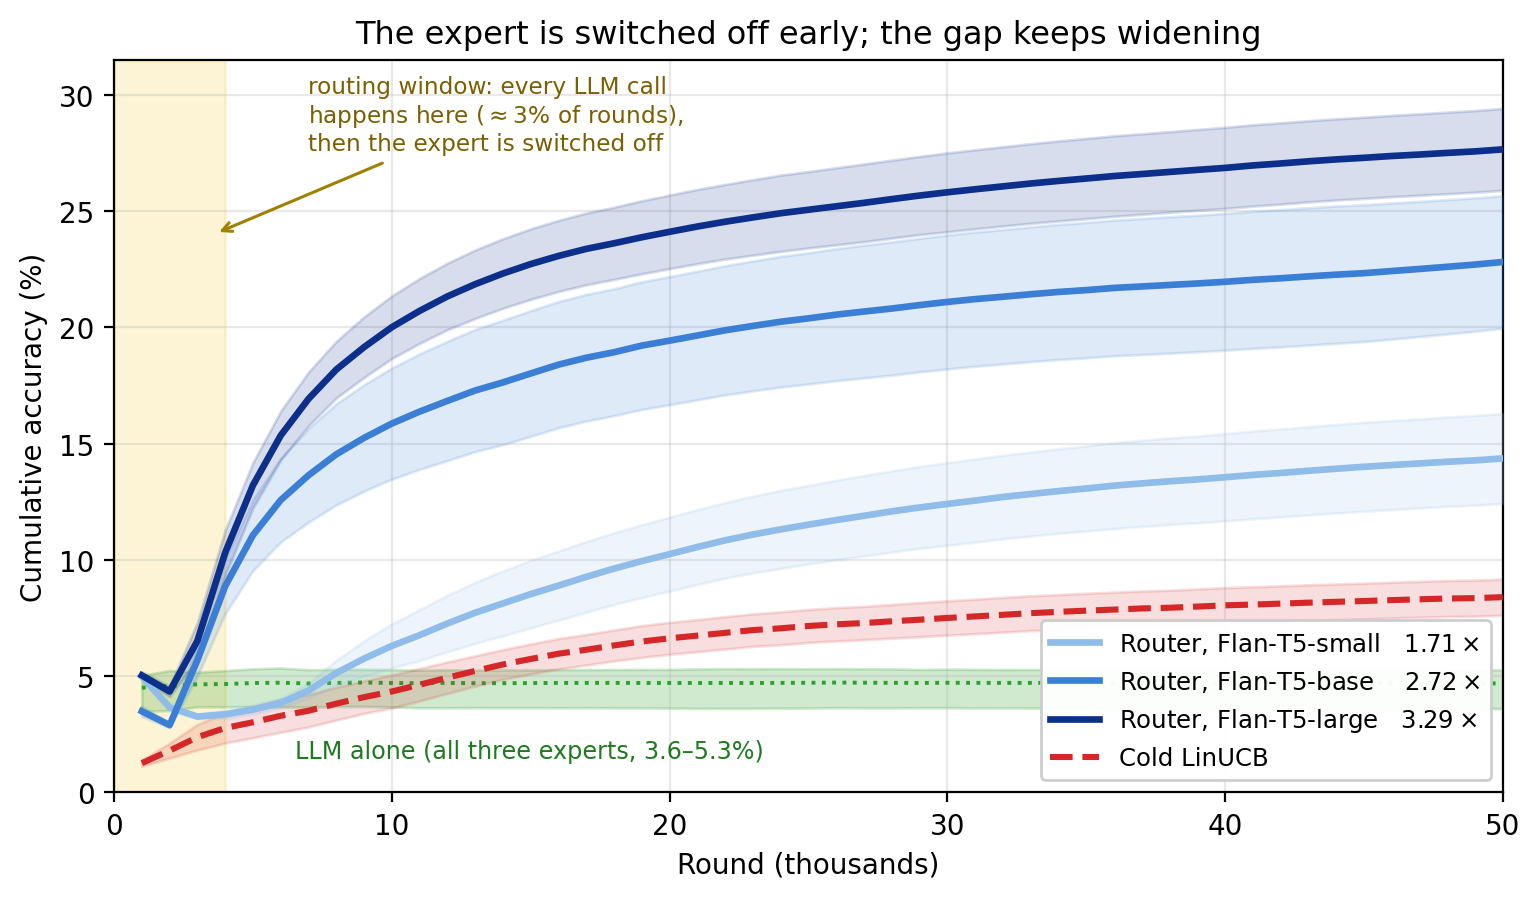
\includegraphics[width=0.85\linewidth]{multiplication.png}
\caption{Learning dynamics on AmazonCat-13K (BERT-768d, $c_{\mathrm{LLM}}=100$), mean over
ten seeds with shaded standard error. The shaded window, the first $4{,}000$
rounds, holds at least $99\%$ of the calls to the LLM in every run; the
Router routes a few more rounds afterwards, the last of them between rounds
$1{,}981$ and $8{,}703$ (Appendix~\ref{app:settling-data}). The three Flan-T5 experts (held-out accuracies
$5.20\%$, $3.61\%$ and $5.27\%$, the band at the bottom) are consulted on
equally few rounds, yet their Routers separate by nearly a factor of two; and
$96$--$100\%$ of each Router's advantage over cold LinUCB, counted in correct
answers, accrues after its last routed round: the saving is collected on the
tail.}
\label{fig:amazon-dynamics}
\end{figure}

\subsection{Tuned Baselines}
\label{app:tuned}

Cold LinUCB is tuned on seeds $11$--$20$ in two steps and evaluated on seeds
$1$--$10$. First, with $\lambda=0.1$, sixteen exploration settings: the
schedules $\alpha_t=\max(a,0.9985^t)$ (the default, ``fast''),
$\max(a,0.9995^t)$ (``slow'') and the constant $\alpha_t=a$, with floors
$a\in\{0.01,0.05,0.1,0.2,0.5\}$ and, for the constant schedule, also $a=1$.
Second, $\lambda\in\{0.01,0.1,1,10\}$ at the best setting. The Router is then
run on the tuned learner with $c_{\mathrm{LLM}}\in\{c_0/10,c_0,10c_0\}$, $c_0$ the value
selected at the default setting ($100$ on BERT, $0.1$ on BGE), selected on seeds $11$--$20$ by mean Router
accuracy over the three experts. On BERT the tuning seeds rank the default
twelfth of sixteen ($8.28\%$ against $11.34\%$ for the best, fast with floor
$0.05$), keep $\lambda=0.1$ ($11.34\%$, against $7.50\%$, $10.30\%$ and
$8.70\%$ at $\lambda=0.01,1,10$), and select $c_{\mathrm{LLM}}=10^3$ ($21.21\%$, against
$20.92\%$ at $10^2$ and $18.77\%$ at $10$). On the evaluation seeds the gain
of the tuned setting disappears (Table~\ref{tab:tuned}): cold LinUCB's
accuracy varies from seed to seed far more than between exploration settings,
because it is decided by which category the learner settles on. On BGE the
best setting is the constant schedule with floor $0.2$ and $\lambda=0.01$
($39.31\%$ on the tuning seeds, against $34.77\%$ at the default), and the
improvement carries over to the evaluation seeds. The tuning seeds then
select $c_{\mathrm{LLM}}=0.1$ for the Router ($48.10\%$, against $42.10\%$ at $0.01$ and
$23.65\%$ at $1$). At the default setting our simulator reproduces the BGE
cold LinUCB of Table~\ref{tab:bge-main} exactly ($32.59\%$).

\paragraph{Category-term features.} On BERT we also append the category
embedding to the features, $\phi(x,a)=[x\odot z_a,\,z_a]$ ($d=1{,}536$), which
lets the learner represent how often a category is right whatever the
context. Cold LinUCB is tuned again on seeds $11$--$20$ over the three best
exploration settings of the first step and the default, at $\lambda=0.1$: fast
with floor $0.05$ scores $15.97\%$, against $12.81\%$ (slow, $0.1$), $12.07\%$
(slow, $0.01$) and $11.32\%$ (the default). The Router is then run at that
setting with $c_{\mathrm{LLM}}\in\{10,10^2,10^3\}$ and the tuning seeds select $10^2$
($38.23\%$, against $36.12\%$ and $34.04\%$). As with the original features,
the selected cold setting does not carry over to the evaluation seeds: the
default schedule scores higher there ($15.60\%$ against $12.56\%$), and
Table~\ref{tab:tuned} reports both.

\begin{table}[ht]
\centering
\caption{Default and tuned baselines on AmazonCat-13K, seeds $1$--$10$, mean
$\pm$ standard deviation. \emph{Default} is the setting of
Section~\ref{sec:exp-setup} (the rows of Tables~\ref{tab:amazon-results} and~\ref{tab:bge-main});
\emph{tuned} is selected on seeds $11$--$20$ as described in the text. The
Router on a tuned learner uses the same exploration and $\lambda$ as the cold
learner it is compared with. Mult.\ is the accuracy multiplier with the regret
ratio in parentheses, measured against the cold LinUCB of the same block;
settle counts runs that settle on the dominant category. The default BGE
Router rows are those of Table~\ref{tab:bge-main}. \emph{Category
term} uses the features $[x\odot z_a,z_a]$; its Router is compared with the
selected cold setting, and the default-schedule cold learner on the same
features is listed for reference.}
\label{tab:tuned}
\small
\setlength{\tabcolsep}{3pt}
\begin{tabular}{@{}lllccc@{}}
\toprule
Features & Learner & Policy & Accuracy & Mult. & Settle \\
\midrule
\multirow{13}{*}{BERT-768d} & \multirow{4}{*}{default} & cold LinUCB & $8.39\pm2.46\%$ & --- & $0/10$ \\
& & Router, Flan-T5-small & $14.37\pm6.12\%$ & $1.71\times$ ($1.07$) & $2/10$ \\
& & Router, Flan-T5-base & $22.80\pm9.00\%$ & $2.72\times$ ($1.19$) & $8/10$ \\
& & Router, Flan-T5-large & $27.64\pm5.56\%$ & $3.29\times$ ($1.27$) & $9/10$ \\
\cmidrule(lr){2-6}
& \multirow{4}{*}{tuned} & cold LinUCB & $8.37\pm5.23\%$ & --- & $1/10$ \\
& & Router, Flan-T5-small & $17.30\pm7.77\%$ & $2.07\times$ ($1.11$) & $4/10$ \\
& & Router, Flan-T5-base & $24.94\pm1.09\%$ & $2.98\times$ ($1.22$) & $10/10$ \\
& & Router, Flan-T5-large & $25.35\pm0.94\%$ & $3.03\times$ ($1.23$) & $10/10$ \\
\cmidrule(lr){2-6}
& \multirow{5}{*}{\shortstack[l]{category\\term}} & cold LinUCB, default schedule & $15.60\pm6.59\%$ & --- & $7/10$ \\
& & cold LinUCB & $12.56\pm5.89\%$ & --- & $2/10$ \\
& & Router, Flan-T5-small & $30.46\pm7.82\%$ & $2.42\times$ ($1.26$) & $4/10$ \\
& & Router, Flan-T5-base & $38.02\pm4.48\%$ & $3.03\times$ ($1.41$) & $10/10$ \\
& & Router, Flan-T5-large & $42.41\pm2.97\%$ & $3.38\times$ ($1.52$) & $10/10$ \\
\midrule
\multirow{8}{*}{BGE-1024d} & \multirow{4}{*}{default} & cold LinUCB & $32.59\pm5.00\%$ & --- & $2/10$ \\
& & Router, Qwen-0.5B & $32.62\pm6.33\%$ & $1.00\times$ ($1.00$) & $4/10$ \\
& & Router, Qwen-3B & $40.20\pm4.45\%$ & $1.23\times$ ($1.13$) & $8/10$ \\
& & Router, Qwen-7B & $38.71\pm6.38\%$ & $1.19\times$ ($1.10$) & $7/10$ \\
\cmidrule(lr){2-6}
& \multirow{4}{*}{tuned} & cold LinUCB & $43.25\pm5.36\%$ & --- & $7/10$ \\
& & Router, Qwen-0.5B & $51.44\pm1.58\%$ & $1.19\times$ ($1.17$) & $10/10$ \\
& & Router, Qwen-3B & $42.93\pm0.32\%$ & $0.99\times$ ($0.99$) & $10/10$ \\
& & Router, Qwen-7B & $51.59\pm0.12\%$ & $1.19\times$ ($1.17$) & $10/10$ \\
\bottomrule
\end{tabular}
\end{table}

\subsection{Coverage and the Transfer}
\label{app:amazon-transfer}
\label{app:two-channel}

Section~\ref{sec:two-channels} says where that difference can live. The three
experts cover the same directions to within $5\%$: summed over the routed
rounds, the coverage of the directions cold LinUCB is trapped on is
$1.40\times10^5$, $1.46\times10^5$ and $1.47\times10^5$, at prices
$9.5\times10^{-3}$, $1.03\times10^{-2}$ and $1.04\times10^{-2}$, so the price
ratio of Theorem~\ref{thm:general-price-full}, measured after the run, is $1.73$,
$1.59$ and $1.58$ for the three---close to one another, and ordered opposite
to the observed accuracy multipliers. We compute it from per-round logs, taking for $U$
the leading directions of the features cold LinUCB played on rounds it lost
after routing stopped, in place of certified arms. The streams are outside
the theorem's setting, so this is an explanatory statistic rather than a
bound the theorem certifies, and by construction it is blind to the
transfer. It bounds the regret ratio, and the observed regret ratios lie
below it for every expert; since the real stream is outside the theorem's
setting we read this as consistency, not confirmation. Since coverage does
not separate the experts, we test directly whether the transfer does, and
Figure~\ref{fig:two-channel} shows that it does (full numbers and tests in
Table~\ref{tab:two-channel}).

The comparison is a replay in which the routed rounds are held fixed. For
each expert and seed, three versions of the learner run in lockstep on the
same stream: the full Router, which decides which rounds are routed, and two
ablated learners that route exactly the same rounds and play the expert's
answer there, whether or not their own confidence would have routed them. On
every other round each learner plays its own LinUCB choice and sees the true
reward. The three versions therefore have the same routed rounds, the same
routed actions and the same routed covariance, and differ only in what the
routed rounds add to the response sum; the full version reproduces the
Router of Table~\ref{tab:amazon-results} exactly. Removing $m$ collapses the
spread of the experts' mean per-seed accuracy multipliers from $1.74$ to $0.50$ and
turns every significant pairwise difference into a null result: large over
small falls from $t=5.18$ to $t=1.33$. Suppressing the response sum on the
routed rounds gives the same collapse, to a spread of $0.01$; and the two
transfer-free conditions do not differ from each other on any expert (paired
$t=-0.66$, $+0.64$, $+0.46$). Removing the transfer costs each expert in
proportion to what it gained: the per-seed accuracy multiplier falls by $2.04$ for
large ($t=4.57$), $1.27$ for base ($t=3.94$) and $0.70$ for small
($t=2.51$). Whether a run settles on the dominant category
(Appendix~\ref{app:dominant}) follows the same pattern: $2$, $8$ and $9$ of
ten runs with the transfer, and at most $2$ of ten for any expert without
it. A third route to the same conclusion
replaces the reward by $\langle\theta_{\mathrm{or}},\phi\rangle+\mathcal
N(0,\varsigma^2)$, making the model well specified so that
Observation~\ref{prop:response-sum} applies up to the Router's adaptive
choice of routed rounds: at
$\varsigma\in\{0.001,0.01,0.499\}$ the three experts' regret ratios, measured
against the oracle's best action, span $0.019$, $0.010$ and $0.030$, against
$0.197$ on the real reward; the ratios themselves lie between $0.97$ and
$1.09$. Under linear rewards the experts are interchangeable, exactly as
predicted.

\textbf{Where the regret goes.} On the regret scale coverage and the transfer
have very different sizes. With the response sum suppressed on the routed
rounds, coverage alone gives regret ratios $1.035$, $1.029$ and $1.019$:
about $2$ to $3.5\%$ less regret than cold LinUCB, indistinguishable across
experts, and below the price ratio for each, consistent with
Theorem~\ref{thm:general-price-full} although the stream is outside its setting.
The full Router gives $1.070$, $1.187$ and $1.266$. For Flan-T5-base and
Flan-T5-large, therefore, almost all of the regret saved is saved by the
transfer, roughly $13$ of $16$ and $19$ of $21$ percentage points, and for
Flan-T5-small about half, $3$ of $6.5$. The separation between experts
survives the change of scale intact: on per-seed regret ratios, large beats
small with paired $t=+5.65$ and base beats small with $t=+3.32$ when the
transfer is present, and neither difference is significant with the transfer
removed ($t=+1.25$, $+1.24$) or the response sum suppressed ($t=-0.47$,
$-0.13$); Figure~\ref{fig:two-channel} shows the same
collapse on the accuracy scale. The price ratio is about the same for the
three experts, as is the coverage gain; it does not predict the size of that
gain, which it bounds loosely.

Finally, the transfer is not a small correction to the estimate at handoff; on
this data it is essentially the whole of it. The ridge oracle assigns a
correct action a score of about $2.5\times10^{-3}$ where the reward is $1$, so
the residuals dominate: $\|m\|/\|\widehat\theta_{\tau+1}\|=0.9998$, and the
identity of Equation~\eqref{eq:transfer} holds on the logged trajectories
to $1.2\times10^{-14}$. Stripping $m$ makes the three estimates agree to four
decimals in held-out ranking quality ($0.2058$, $0.2058$, $0.2057$), while the
transfers themselves separate the experts with the same resolution the
accuracy multipliers have: base and large each beat small ($t=3.12$, $t=2.56$) and are
indistinguishable from one another ($t=0.36$), which is the pair the
accuracy multipliers also cannot separate.

\begin{table}[ht]
\centering
\caption{Separating coverage from the transfer on AmazonCat/BERT-768d, ten seeds,
with the routed rounds held fixed: all three versions route exactly the rounds
the full Router chose and play the expert's answer there, so their routed
covariance is identical. In \emph{full} a routed round also adds its observed
reward to the response sum, as the Router does. In \emph{transfer removed} it
adds the expert-independent part: the learner is fed
$\langle\theta_{\mathrm{or}},\phi\rangle$ instead of the observed reward on
the routed rounds, which deletes $m$ of Equation~\eqref{eq:transfer}. In
\emph{no response sum} it adds nothing to the response sum. On every other
round each version plays its own LinUCB choice. Accuracy multipliers are
Router over cold LinUCB ($8.40\%$), with the regret ratio in
parentheses. The spread is the largest minus the smallest of the three
experts' mean per-seed accuracy multipliers; $t$-statistics are paired over seeds, on
each scale, $t^\star=2.26$. With the transfer present the experts separate;
without it, by either mechanism, no pairwise difference survives.}
\label{tab:two-channel}
\footnotesize
\setlength{\tabcolsep}{3pt}
\begin{tabular}{@{}lcccccc@{}}
\toprule
& \multicolumn{3}{c}{Router accuracy} & \multicolumn{3}{c}{Accuracy multiplier over cold} \\
\cmidrule(lr){2-4}\cmidrule(lr){5-7}
LLM & full & transfer removed & no response sum & full & transfer removed & no response sum \\
\midrule
Flan-T5-small & $14.37\pm6.12\%$ & $9.71\pm4.18\%$  & $11.53\pm6.61\%$ & $1.71\times$ ($1.07$) & $1.16\times$ ($1.01$) & $1.37\times$ ($1.04$) \\
Flan-T5-base  & $22.80\pm9.00\%$ & $12.56\pm5.66\%$ & $11.02\pm6.86\%$ & $2.72\times$ ($1.19$) & $1.50\times$ ($1.05$) & $1.31\times$ ($1.03$) \\
Flan-T5-large & $27.64\pm5.56\%$ & $12.49\pm6.35\%$ & $10.10\pm5.08\%$ & $3.29\times$ ($1.27$) & $1.49\times$ ($1.05$) & $1.20\times$ ($1.02$) \\
\midrule
\multicolumn{4}{@{}l}{runs settling on $1471$ (small / base / large)} & $2/8/9$ & $1/2/2$ & $1/2/1$ \\
\multicolumn{4}{@{}l}{spread of mean per-seed accuracy multipliers} & $1.74$ & $0.50$ & $0.01$ \\
\multicolumn{4}{@{}l}{large $-$ small, paired $t$} & $\mathbf{+5.18}$ & $+1.33$ & $+0.01$ \\
\multicolumn{4}{@{}l}{base $-$ small, paired $t$} & $\mathbf{+3.03}$ & $+1.36$ & $+0.03$ \\
\multicolumn{4}{@{}l}{large $-$ small, paired $t$, regret ratio} & $\mathbf{+5.65}$ & $+1.25$ & $-0.47$ \\
\multicolumn{4}{@{}l}{base $-$ small, paired $t$, regret ratio} & $\mathbf{+3.32}$ & $+1.24$ & $-0.13$ \\
\bottomrule
\end{tabular}
\end{table}

\subsection{BGE Features}
\label{app:bge}

\begin{table}[ht]
\centering
\caption{AmazonCat-13K with BGE-1024d features and Qwen2.5 experts at the
default learner, $T=50{,}000$, mean $\pm$ standard deviation over seeds
$1$--$10$, $c_{\mathrm{LLM}}=0.1$ selected on seeds $11$--$20$. Columns as in
Table~\ref{tab:amazon-results}; LLM\% is the share of rounds routed to the
LLM. The two larger experts gain significantly (paired $t=3.92$ and $2.59$
against cold) and the smallest does not ($t=0.01$). The tuned rows are in
Table~\ref{tab:tuned}.}
\label{tab:bge-main}
\small
\setlength{\tabcolsep}{3pt}
\begin{tabular}{@{}lcccccc@{}}
\toprule
LLM & LLM acc.\ & Cold LinUCB & Router & LLM\% & Acc.\ mult.\ & Regret ratio \\
\midrule
Qwen-0.5B  & $21.38\%$ & $32.59\pm5.00\%$ & $32.62\pm6.33\%$ & $0.04\%$  & $1.00\times$ & $1.00$ \\
Qwen-3B  & $22.39\%$ & $32.59\pm5.00\%$ & $\mathbf{40.20\pm4.45\%}$ & $0.05\%$  & $\mathbf{1.23\times}$ & $\mathbf{1.13}$ \\
Qwen-7B  & $27.17\%$ & $32.59\pm5.00\%$ & $38.71\pm6.38\%$ & $0.05\%$  & $1.19\times$ & $1.10$ \\
\bottomrule
\end{tabular}
\end{table}

\begin{table}[ht]
\centering
\caption{Confidence sweep on the BGE-1024d configurations, tuning seeds
$11$--$20$, which select $c_{\mathrm{LLM}}$. At the
$c_{\mathrm{LLM}}=100$ used for BERT the expert width $u^{(1)}=\|\phi\|/\sqrt{c_{\mathrm{LLM}}}$ is
permanently below LinUCB's, the Router never routes, and it equals the
LLM exactly on every seed ($I_\tau=0$, zero variance). Lowering $c_{\mathrm{LLM}}$ raises the
expert's width and restores routing. On AmazonCat, where cold LinUCB is
strong, the Router at $c_{\mathrm{LLM}}=0.1$ beats it while routing $0.05\%$ of rounds, and
the same $c_{\mathrm{LLM}}$ reproduces the gain on the evaluation seeds
(Table~\ref{tab:bge-main}); at $c_{\mathrm{LLM}}\ge1$ it is dragged down toward a
weaker expert. On WikiLinks the expert is
already better than the learner (cold
LinUCB $18.88\%$ on these seeds, LLMs $18.72\%$, $29.47\%$ and $38.74\%$): the
selected $c_{\mathrm{LLM}}=10$ routes every round, so the Router is the expert, and at
$c_{\mathrm{LLM}}=1$, where the Router hands back, the Router falls well below the two
larger experts.}
\label{tab:bge-csweep}
\scriptsize
\setlength{\tabcolsep}{4pt}
\begin{tabular}{@{}llccccccc@{}}
\toprule
& & \multicolumn{3}{c}{routed \%} & \multicolumn{3}{c}{Router accuracy} & \\
\cmidrule(lr){3-5}\cmidrule(lr){6-8}
Dataset & $c_{\mathrm{LLM}}$ & 0.5B & 3B & 7B & 0.5B & 3B & 7B & best mult.\ \\
\midrule
\multirow{4}{*}{AmazonCat} & $0.01$ & $0.0$ & $0.0$ & $0.0$ & $34.77$ & $34.77$ & $34.77$ & $1.00\times$ \\
 & $\mathbf{0.1}$ & $0.04$ & $0.05$ & $0.05$ & $33.84$ & $39.68$ & $\mathbf{40.63}$ & $\mathbf{1.17\times}$ \\
 & $1$  & $75.2$ & $71.9$ & $73.5$ & $28.09$ & $29.26$ & $36.50$ & $1.05\times$ \\
 & $10$ & $100$ & $100$ & $100$ & $21.38$ & $22.39$ & $27.17$ & $0.78\times$ \\
\cmidrule(lr){1-9}
\multirow{5}{*}{WikiLinks} & $0.01$ & $0.0$ & $0.0$ & $0.0$ & $18.88$ & $18.88$ & $18.88$ & $1.00\times$ \\
 & $0.1$ & $0.002$ & $0.002$ & $0.002$ & $18.88$ & $18.87$ & $18.88$ & $1.00\times$ \\
 & $1$  & $13.6$ & $13.6$ & $13.7$ & $18.98$ & $20.55$ & $21.89$ & $1.01\times$ \\
 & $\mathbf{10}$ & $100$ & $100$ & $100$ & $18.72$ & $29.47$ & $\mathbf{38.74}$ & $1.00\times$ \\
 & $100$ & $100$ & $100$ & $100$ & $18.72$ & $29.47$ & $38.74$ & $1.00\times$ \\
\bottomrule
\end{tabular}
\end{table}

\textbf{BGE-1024d.} At the $c_{\mathrm{LLM}}=100$ used for BERT the Router never hands
back and equals the LLM, a failure of the hyperparameter rather than evidence
about $I_\tau$, so the tuning seeds sweep $c_{\mathrm{LLM}}$ down
(Table~\ref{tab:bge-csweep}) and select $0.1$. On the evaluation seeds
(Table~\ref{tab:bge-main}) the Router routes $0.05\%$ of rounds, and the two
larger Qwen2.5 experts gain significantly while the smallest does not move.
Where there is a gain, the accounting has the BERT shape: $A_\tau$ is $5$ and
$6$ correct answers while $I_\tau$ is $3{,}801$ and $3{,}056$, positive on $9$
and $8$ of the ten seeds, against $I_\tau=13$ for Qwen-0.5B. The gains are
smaller than on BERT because cold LinUCB on BGE features already settles on
the dominant category in $7$ of $20$ seeds (Appendix~\ref{app:dominant}). On
WikiLinks the Qwen experts are better than the learner, so the selected
$c_{\mathrm{LLM}}=10$ routes every round and the Router equals the expert
($I_\tau=B_\tau=0$); at $c_{\mathrm{LLM}}=1$, the largest value at which it hands
back, it routes $14\%$ of rounds and reaches only $20.55\%$ and $21.89\%$ with
Qwen-3B and Qwen-7B.

\subsection{OneShotWikiLinks-311}
\label{app:wiki}

\textbf{Setup.} $622{,}000$ context--entity pairs over $311$ entities.
\emph{Flan-T5 (BERT-768d features)}: embeddings from
\texttt{bert-base-nli-mean-tokens}, joint feature $\phi(x,a)=x\odot a\in\mathbb R^{768}$,
expert Flan-T5 \citep{chung2024scaling} at 60M/250M/780M.
\emph{Qwen2.5 (BGE-1024d features)}: embeddings from
\texttt{BAAI/bge-large-en-v1.5} \citep{xiao2024c}, expert Qwen2.5-Instruct
\citep{hui2024qwen2} at 0.5B/3B/7B.

\begin{table}[ht]
\centering
\caption{Final cumulative accuracy on OneShotWikiLinks-311, mean$\pm$std over
seeds $1$--$10$, at the $c_{\mathrm{LLM}}$ chosen on seeds $11$--$20$: $10^4$ for Flan-T5
(Table~\ref{tab:wiki-csweep}) and $10$ for Qwen2.5 (Table~\ref{tab:bge-csweep}).
LLM accuracy and cold LinUCB do not depend on $c_{\mathrm{LLM}}$. Mult.\ is the accuracy
multiplier Router/$\max$(LLM, Cold); the regret ratio is within $0.01$ of one
on every row. The lift column is the Router's gain over cold LinUCB in
percentage points. The Flan-T5 Routers consult the expert on $14.7\%$,
$13.4\%$ and $13.8\%$ of rounds; the Qwen2.5 Routers on every round, so they
equal the expert exactly.}
\label{tab:wiki-results}
\small
\begin{tabular}{@{}llccccc@{}}
\toprule
Family & Size & LLM & Cold LinUCB & Router & Lift (pp) & Mult.\ \\
\midrule
\multirow{3}{*}{Flan-T5} & small (60M) & $7.16\%$  & $10.71\pm 0.04\%$ & $10.71\pm 0.03\%$ & $0.00$ & $1.00\times$ \\
& base (250M)   & $10.56\%$ & $10.71\pm 0.04\%$ & $11.29\pm 0.02\%$ & $+0.58$ & $1.05\times$ \\
& large (780M)  & $12.43\%$ & $10.71\pm 0.04\%$ & $11.56\pm 0.04\%$ & $+0.85$ & $0.93\times$ \\
\midrule
\multirow{3}{*}{Qwen2.5} & 0.5B  & $18.72\%$ & $18.90\pm 0.02\%$ & $18.72\pm0.00\%$ & $-0.18$ & $0.99\times$ \\
& 3B  & $29.47\%$ & $18.90\pm 0.02\%$ & $29.47\pm0.00\%$ & $+10.57$ & $1.00\times$ \\
& 7B  & $38.74\%$ & $18.90\pm 0.02\%$ & $38.74\pm0.00\%$ & $+19.85$ & $1.00\times$ \\
\bottomrule
\end{tabular}
\end{table}

\textbf{Results.} Table~\ref{tab:wiki-results} reports final cumulative
accuracy at the selected $c_{\mathrm{LLM}}$. With Flan-T5 the Router routes $13$--$15\%$
of rounds to the LLM. Routing is driven by feature geometry, not by
reward: all three Flan-T5 sizes are routed on nearly the same share of
rounds at every $c_{\mathrm{LLM}}$ (Table~\ref{tab:wiki-csweep}) despite a large spread
in accuracy. The gain over cold LinUCB is significant for Flan-T5-base and
Flan-T5-large (paired $t=36.4$ and $52.2$, since the seeds vary little on
$622{,}000$ rounds) but small, and the Router stays below Flan-T5-large itself.

\textbf{Confidence sweep.} To rule out a suboptimal $c_{\mathrm{LLM}}$, the Flan-T5
configurations are swept over $c_{\mathrm{LLM}}\in\{1,10,10^2,10^3,10^4\}$ on the tuning seeds
$11$--$20$ (Table~\ref{tab:wiki-csweep}), and the Qwen configurations over
$c_{\mathrm{LLM}}\in\{0.01,0.1,1,10,100\}$ (Table~\ref{tab:bge-csweep}).

\begin{table}[ht]
\centering
\caption{Confidence sweep on the WikiLinks Flan-T5 (BERT-768d) configurations,
tuning seeds $11$--$20$: share of rounds routed to the LLM and final Router
accuracy at each $c_{\mathrm{LLM}}$, mean over seeds. Cold LinUCB does not depend on $c_{\mathrm{LLM}}$
($10.70\%$ on these seeds); the LLMs score $7.16\%$, $10.56\%$ and $12.43\%$.
Best mult.\ is the largest Router accuracy over $\max\{$LLM, cold$\}$ among the
three experts. Mean Router accuracy over the experts is highest at
$c_{\mathrm{LLM}}=10^4$ ($11.18\%$, against $11.05\%$ at $10^3$ and $10.86\%$ at $10^2$),
which is therefore the value evaluated on seeds $1$--$10$. At that value the
Router consults the LLM on about $14\%$ of rounds and moves toward the LLM's
own accuracy rather than beating both: it gains on the two experts that beat
cold LinUCB and stays below Flan-T5-large itself.}
\label{tab:wiki-csweep}
\scriptsize
\setlength{\tabcolsep}{4pt}
\begin{tabular}{@{}lccccccc@{}}
\toprule
& \multicolumn{3}{c}{routed \%} & \multicolumn{3}{c}{Router accuracy} & \\
\cmidrule(lr){2-4}\cmidrule(lr){5-7}
$c_{\mathrm{LLM}}$ & small & base & large & small & base & large & best mult.\ \\
\midrule
$1$ & $0.10$ & $0.09$ & $0.10$ & $10.77$ & $10.79$ & $10.82$ & $1.01\times$ \\
$10$ & $0.14$ & $0.14$ & $0.14$ & $10.78$ & $10.81$ & $10.82$ & $1.01\times$ \\
$10^2$ & $0.29$ & $0.27$ & $0.27$ & $10.83$ & $10.85$ & $10.90$ & $1.01\times$ \\
$10^3$ & $1.61$ & $1.47$ & $1.52$ & $10.97$ & $11.06$ & $11.13$ & $1.03\times$ \\
$\mathbf{10^4}$ & $14.7$ & $13.4$ & $13.8$ & $10.71$ & $11.26$ & $\mathbf{11.55}$ & $\mathbf{1.05\times}$ \\
\bottomrule
\end{tabular}
\end{table}

The decomposition explains the shape. For Flan-T5 the routed rounds do leave
usable data---$I_\tau$ is $2{,}392$, $2{,}859$ and $3{,}098$ correct answers and is
positive on all ten seeds---so the expert's data is not aimed at the wrong
directions. Unlike on AmazonCat,
$A_\tau$ is not negligible: it is $-2{,}395$, $732$ and $2{,}201$, and for
Flan-T5-small the expert loses on the routed rounds almost exactly what its
data gains afterwards, so the Router ends where cold LinUCB does. The gain stays small
because there is little for the expert to steer the learner toward: the most
frequent of the $311$ entities covers $0.36\%$ of contexts, whereas on
AmazonCat one category covers $29.8\%$ (Section~\ref{sec:amazon}). For Qwen the expert is far better than the
learner ($29$--$39\%$ against $19\%$): at the selected $c_{\mathrm{LLM}}$ every round
is routed, the whole difference from cold LinUCB is $A_\tau$ ($-1{,}122$,
$65{,}772$ and $123{,}441$ correct answers), and $I_\tau=B_\tau=0$.

\subsection{Other Routing Rules}
\label{app:routers}

The Router differs from the randomized CORRAL master of
\citet{agarwal2017corralling} and the CORRAL-style routing of
\citet{chen2024llmdecision} only in how it chooses the routed rounds; all
feed every observation to the bandit learner, so the decomposition applies
to each, and any difference between them appears in $A_\tau$ or in which
residuals their routed sets collect. Table~\ref{tab:baselines} runs both alternatives.

\begin{table}[ht]
\centering
\caption{Alternative routing mechanisms on AmazonCat-13K (BERT-768d,
$c_{\mathrm{LLM}}=100$), ten seeds, paired on seed with the Router. CORRAL is the randomized
log-barrier master of \citet{agarwal2017corralling} with importance-weighted
updates; the offline arms spend $\tau$ expert pulls on contexts drawn from
\emph{outside} the online stream and then run plain LinUCB, so their
acquisition is not charged as regret and $A_\tau=0$ identically.
$\tau=1{,}600$ matches the Router's routed count. Cold LinUCB is bit-identical
across all four arms on every seed, so each comparison isolates the router.
The last column is the paired $t$ statistic for the Router minus that arm over the
ten shared seeds ($t^\star=2.26$). Mult.\ is the accuracy multiplier, with
the regret ratio in parentheses.}
\label{tab:baselines}
\small
\setlength{\tabcolsep}{4pt}
\begin{tabular}{@{}llrcccrr@{}}
\toprule
LLM & Routing rule & queries & Accuracy & Mult.\ & $A_\tau$ & $I_\tau$ & $t$ vs.\ Router \\
\midrule
\multirow{4}{*}{Flan-T5-small}
 & Router (Alg.\ 1)    & $1{,}406$  & $14.37\pm6.12\%$ & $1.71\times$ ($1.07$) & $47$   & $2{,}936$ & --- \\
 & CORRAL            & $22{,}860$ & $8.87\pm1.37\%$  & $1.06\times$ ($1.01$) & $-508$ & $744$     & $\mathbf{2.64}$ \\
 & Offline $\tau{=}1{,}600$ & $1{,}600$ & $11.17\pm5.71\%$ & $1.33\times$ ($1.03$) & $0$ & $1{,}386$ & $1.16$ \\
 & Offline $\tau{=}5{,}000$ & $5{,}000$ & $15.95\pm7.11\%$ & $1.90\times$ ($1.09$) & $0$ & $3{,}778$ & $-0.59$ \\
\midrule
\multirow{4}{*}{Flan-T5-base}
 & Router (Alg.\ 1)    & $1{,}570$ & $22.80\pm9.00\%$ & $2.72\times$ ($1.19$) & $27$  & $7{,}178$ & --- \\
 & CORRAL            & $6{,}939$ & $24.44\pm2.39\%$ & $2.91\times$ ($1.21$) & $-23$ & $8{,}045$ & $-0.63$ \\
 & Offline $\tau{=}1{,}600$ & $1{,}600$ & $20.97\pm8.89\%$ & $2.50\times$ ($1.16$) & $0$ & $6{,}286$ & $0.42$ \\
 & Offline $\tau{=}5{,}000$ & $5{,}000$ & $27.29\pm5.17\%$ & $3.25\times$ ($1.26$) & $0$ & $9{,}449$ & $-2.00$ \\
\midrule
\multirow{4}{*}{Flan-T5-large}
 & Router (Alg.\ 1)    & $1{,}597$ & $27.64\pm5.56\%$ & $3.29\times$ ($1.27$) & $53$ & $9{,}571$ & --- \\
 & CORRAL            & $7{,}488$ & $25.42\pm2.31\%$ & $3.03\times$ ($1.23$) & $50$ & $8{,}460$ & $1.49$ \\
 & Offline $\tau{=}1{,}600$ & $1{,}600$ & $26.27\pm7.61\%$ & $3.13\times$ ($1.24$) & $0$ & $8{,}937$ & $0.42$ \\
 & Offline $\tau{=}5{,}000$ & $5{,}000$ & $25.76\pm6.53\%$ & $3.07\times$ ($1.23$) & $0$ & $8{,}681$ & $0.67$ \\
\bottomrule
\end{tabular}
\end{table}

Three things follow. First, no baseline beats the Router significantly on any
expert, and the Router beats CORRAL on Flan-T5-small ($t=2.64$) while issuing
$16\times$ fewer expert queries; on the other two experts CORRAL matches the
Router at four to five times the query budget. Second, the offline arm at a
matched budget of $1{,}600$ pulls is statistically indistinguishable from the
Router on all three experts even though its acquisition is free, so the online
routing decision costs essentially nothing---which is the content of
$A_\tau\approx0$, now visible from the other side. Tripling the free budget to
$5{,}000$ still does not separate the two. Where an alternative does come out
ahead of the Router in the mean, the margin is small, never significant, and
paid for with a much larger budget: CORRAL on Flan-T5-base gains $1.6$
points ($t=-0.63$) with $4.4\times$ the Router's expert queries, and the
offline arm at $\tau=5{,}000$ gains $1.6$ and $4.5$ points on Flan-T5-small
and Flan-T5-base ($t=-0.59$, $-2.00$) only by drawing $3$--$4\times$ as many
expert answers, all collected before the online run begins. None of these
trades buys a reliable improvement, so the Router is the cheapest routing rule in
the comparison and no alternative is significantly better on any expert.

Third, the decomposition survives the change of master: in all twelve rows
$I_\tau$ carries the value and $A_\tau$ is negligible beside it. $A_\tau$ is
where the routing rule shows up: $0$ by construction offline, a few dozen for
the Router, and negative for CORRAL on the two weaker experts ($-508$ and
$-23$). Coverage is not bought by volume: CORRAL routes $16\times$ as many
rounds as the Router on Flan-T5-small and ends with $I_\tau=744$ against the
Router's $2{,}936$.

\section{The Dominant Category on AmazonCat-13K}
\label{app:dominant}

This appendix gives the evidence behind prediction P3 in Section~\ref{sec:amazon}. All numbers are on BERT-768d features
unless stated.

\paragraph{The label distribution.}
On the $50{,}000$ contexts of the online stream the four most frequent of the
$13{,}330$ categories are present on $29.8\%$, $17.0\%$, $11.3\%$ and $7.8\%$
of contexts (category identifiers $1471$, $7961$, $7892$, $7891$). A policy
that always predicts the first scores $29.77\%$; it uses the label
distribution, which an online learner is not given. Context-free bandits that
must discover it do not: over the same stream, $50{,}000$ rounds and seeds
$1$--$10$, UCB1 (one pull of every category first) scores $0.04\%$ and an
optimistic empirical-mean greedy rule $2.31\%$.

\paragraph{Where a run settles.}
We say a run \emph{settles} on a category if that category accounts for more
than $20\%$ of the learner's plays in the last fifth of the horizon. For the
dominant category the classification does not depend on the threshold: on the
runs of Table~\ref{tab:settle}, moving it anywhere between $10\%$ and $30\%$
changes the number of runs that settle on $1471$ by at most one on BERT
features and not at all on BGE features. The counts for the less frequent
categories are more sensitive on BERT, where runs that settle on $7892$
predict it on about a fifth of late rounds. Table~\ref{tab:settle}
reports where runs settle and how accurate the runs that settle on each
category are. On BERT features cold LinUCB settles on the dominant category
in $1$ of $20$ seeds; the two experts with large gains move it there in $17$ of
$20$. On BGE features cold LinUCB already settles there in $7$ of $20$ seeds,
which is why the expert has less to add; there the runs that settle on the
dominant category reach $41.2\%$, above the $29.8\%$ of always predicting
it, so the learner also uses the context. Knowing only where each run
settles predicts mean Router accuracy well: predicting a configuration's
accuracy as the frequency of each settled category times the mean accuracy
of runs settling there in the \emph{other} configurations gives $R^2=0.93$
over $25$ BERT configurations and $R^2=0.93$ over $7$ BGE configurations.
These are every configuration that routes fewer than half the rounds: on
BERT, the Router at $c_{\mathrm{LLM}}\in\{1,10,10^2,10^3\}$, CORRAL, the two offline arms of
Table~\ref{tab:baselines} and the transfer-removed ablation of
Table~\ref{tab:two-channel}, for each of the three experts, plus cold
LinUCB; on BGE, the Router at $c_{\mathrm{LLM}}\in\{0.01,0.1\}$ for each expert, plus cold
LinUCB.

\begin{table}[ht]
\centering
\caption{Where runs settle on AmazonCat-13K (seeds $1$--$20$; BERT at $c_{\mathrm{LLM}}=100$,
BGE at $c_{\mathrm{LLM}}=0.1$). Each cell counts runs that settle on that category; the
percentage under each category is its frequency in the stream. The bottom
block gives the mean final accuracy of the runs, pooled over the four rows,
that settle on each category.}
\label{tab:settle}
\small
\setlength{\tabcolsep}{4pt}
\begin{tabular}{@{}llcccccc@{}}
\toprule
& & $1471$ & $7961$ & $7892$ & $7891$ & & \\
Features & Policy & ($29.8\%$) & ($17.0\%$) & ($11.3\%$) & ($7.8\%$) & none & Accuracy \\
\midrule
\multirow{4}{*}{BERT-768d} & Cold LinUCB & $1$ & $0$ & $9$ & $1$ & $9$ & $8.34\%$ \\
& Flan-T5-small & $3$ & $0$ & $14$ & $0$ & $3$ & $13.71\%$ \\
& Flan-T5-base & $17$ & $0$ & $3$ & $0$ & $0$ & $25.10\%$ \\
& Flan-T5-large & $17$ & $0$ & $3$ & $0$ & $0$ & $26.90\%$ \\
\midrule
\multirow{4}{*}{BGE-1024d} & Cold LinUCB & $7$ & $12$ & $0$ & $0$ & $1$ & $33.68\%$ \\
& Qwen-0.5B & $8$ & $9$ & $0$ & $2$ & $1$ & $33.23\%$ \\
& Qwen-3B & $17$ & $2$ & $0$ & $1$ & $0$ & $39.94\%$ \\
& Qwen-7B & $16$ & $3$ & $0$ & $1$ & $0$ & $39.67\%$ \\
\midrule
\multicolumn{2}{@{}l}{Accuracy of settled runs, BERT} & $28.08\%$ & --- & $11.61\%$ & $6.24\%$ & $5.93\%$ & \\
\multicolumn{2}{@{}l}{Accuracy of settled runs, BGE} & $41.21\%$ & $30.84\%$ & --- & $24.66\%$ & $25.96\%$ & \\
\bottomrule
\end{tabular}
\end{table}

\paragraph{A handful of routed answers decides it.}
Table~\ref{tab:dose} groups every Router run that routes fewer than half the
rounds by the number $k$ of routed rounds on which the expert proposed the
dominant category and was correct, and reports the fraction that settle on
it. On BERT features the fraction rises from $7\%$ at $k=0$ to $80\%$ at
$k=4$, and every one of the $54$ runs with $k\ge5$ settles there. On BGE
features the fraction at $k=0$ is already $43\%$, the rate at which the
learner finds the category by itself, and again every run with $k\ge5$
settles there. The pooled runs span experts, values of $c_{\mathrm{LLM}}$ and, on BERT, the
CORRAL master, so the curve is a property of the learner and the data rather
than of one expert. The three BERT experts differ in exactly this count: in
the $c_{\mathrm{LLM}}=100$ runs the mean $k$ is $0.20$ for Flan-T5-small, $3.70$ for
Flan-T5-base and $4.00$ for Flan-T5-large.

\begin{table}[ht]
\centering
\caption{Runs that settle on the dominant category, by the number $k$ of
correct routed answers on it. BERT: $177$ runs ($c_{\mathrm{LLM}}\in\{1,10,10^2,10^3\}$ and
CORRAL). BGE: $99$ runs ($c_{\mathrm{LLM}}\in\{0.01,0.1\}$).}
\label{tab:dose}
\small
\begin{tabular}{@{}lcccccc@{}}
\toprule
$k$ & $0$ & $1$ & $2$ & $3$ & $4$ & $\ge5$ \\
\midrule
BERT-768d & $3/45$ ($7\%$) & $11/29$ ($38\%$) & $9/17$ ($53\%$) & $13/17$ ($76\%$) & $12/15$ ($80\%$) & $54/54$ ($100\%$) \\
BGE-1024d & $25/58$ ($43\%$) & $3/3$ & $5/9$ & $6/8$ & $8/9$ & $12/12$ ($100\%$) \\
\bottomrule
\end{tabular}
\end{table}

\paragraph{Controlled test.}
Table~\ref{tab:inject} changes the expert's answers on a fixed set of $15$
contexts and nothing else. The runs use an exact re-implementation of the
Router and of cold LinUCB, checked to make the same choice as the
experimental runner on every round of a $3{,}000$-round comparison, on
$10{,}000$ held-out contexts that do not appear in the online stream, with a
horizon of $10{,}000$ rounds and $20$ seeds; the seed fixes the order of the
contexts and is shared across conditions, so every comparison is paired.
Accuracy multipliers are relative to cold LinUCB on the same runs ($4.63\%$).
\emph{$+15$ on $1471$} replaces $15$ wrong answers of Flan-T5-small by the
dominant category on contexts that contain it. \emph{$+15$ random} gives the
same number of correct answers, on the same contexts where possible, on a
uniformly chosen true category other than $1471$. \emph{$+15$ on $7961$}
gives $15$ correct answers on the second most frequent category.
\emph{$-15$ on $1471$} replaces the $15$ correct dominant-category answers of
Flan-T5-large by wrong answers. The first three conditions raise held-out
accuracy by the same $0.15$ points; only the category differs.
\emph{$+15$ on $1471$, reward hidden} uses the same answers as \emph{$+15$ on
$1471$}, but when the Router routes one of the $15$ changed contexts the
learner adds the answer's feature vector to its design matrix and nothing to
its response sum: the change adds coverage along the dominant category and no
transfer. Strictly, adding nothing to the response sum is what a reward of
$0$ would do, a transfer of $-\langle\theta_{\mathrm{or}},\phi\rangle$
relative to the linear model; since the ridge oracle scores these answers at
about $2.5\times10^{-3}$ (Appendix~\ref{app:amazon-transfer}), this is
numerically the same as removing the transfer. Only $2.15$ of the $15$ changed answers are routed per seed on
average (none in one seed), so the whole effect of the intervention passes
through two or three routed rounds.

\begin{table}[ht]
\centering
\caption{Changing $15$ of the expert's $10{,}000$ held-out answers. Tests are
paired over $20$ seeds against the unmodified expert: a paired $t$-test on
Router accuracy and an exact McNemar test on whether the run settles on
$1471$.}
\label{tab:inject}
\small
\setlength{\tabcolsep}{4pt}
\resizebox{\linewidth}{!}{%
\begin{tabular}{@{}llccccc@{}}
\toprule
Expert & Change & Expert acc. & Router acc. & Mult. & Settle on $1471$ & $p$ (acc.\ / settle) \\
\midrule
\multirow{5}{*}{Flan-T5-small} & none & $5.34\%$ & $6.14\%$ & $1.33\times$ & $1/20$ & --- \\
& $+15$ random & $5.49\%$ & $7.63\%$ & $1.65\times$ & $2/20$ & $0.15$ / $1.00$ \\
& $+15$ on $7961$ & $5.49\%$ & $9.39\%$ & $2.03\times$ & $3/20$ & $0.010$ / $0.50$ \\
& $+15$ on $1471$ & $5.49\%$ & $\mathbf{12.10\%}$ & $\mathbf{2.62\times}$ & $\mathbf{8/20}$ & $\mathbf{0.002}$ / $\mathbf{0.016}$ \\
& $+15$ on $1471$, reward hidden & $5.49\%$ & $6.83\%$ & $1.48\times$ & $2/20$ & $0.47$ / $1.00$ \\
\midrule
\multirow{2}{*}{Flan-T5-large} & none & $5.32\%$ & $13.79\%$ & $2.98\times$ & $10/20$ & --- \\
& $-15$ on $1471$ & $5.17\%$ & $10.09\%$ & $2.18\times$ & $6/20$ & $0.067$ / $0.39$ \\
\bottomrule
\end{tabular}}
\end{table}

Hiding the reward of the added answers removes the gain: the Router falls
back to $1.48\times$, not significantly different from the unmodified expert,
and significantly below the same answers with their rewards (paired $t=3.46$,
$p=0.003$; settling $8/20$ against $2/20$, McNemar $p=0.031$). Since only
about two changed answers are routed per run, the comparison is between two
or three rewarded answers on the dominant category, which are enough to move
the learner there and double the accuracy multiplier, and the same two or three
answers with their rewards hidden, which leave the learner where it was. What
the learner uses is the reward, not the coverage along the category. At equal
accuracy, the gain grows with the frequency of the category the
added answers point to: none for random categories, a significant gain for
the second most frequent category (where $5$ of $20$ runs settle on that
category instead), and the largest gain for the dominant one. Removing the
dominant-category answers from Flan-T5-large lowers its accuracy multiplier but not
significantly; its other answers still lead $6$ of $20$ runs to the
dominant category. Individual seeds are sensitive to any change in the
routed data, which can tip a run toward or away from a category, so we
compare rates over seeds rather than reading individual pairs.

\paragraph{The same test on the evaluation stream.}
Table~\ref{tab:inject50k} repeats the test on the $50{,}000$-round stream and
seeds $1$--$10$ of Table~\ref{tab:amazon-results}, with the same simulator.
To keep the same share of the stream, $75$ of Flan-T5-small's wrong answers
are changed, again $+0.15$ points of expert accuracy ($5.20\%$ to $5.35\%$);
the unmodified row is the Router of Table~\ref{tab:amazon-results}, and cold
LinUCB is the same $8.40\%$. The conditions are those of
Table~\ref{tab:inject}: \emph{$+75$ on $1471$}, the same answers with their
rewards hidden, and $+75$ correct answers on random categories other than
$1471$. The Router routes $2.6$ of the $75$ changed answers per seed on
average (none in one seed), about the same number as on the held-out stream,
since it consults the expert almost only in the first few thousand rounds.
The result is the same: rewarded answers on the dominant category raise the
accuracy multiplier from $1.71\times$ to $2.56\times$ and settling from $2$ to $7$ of
ten runs, while the same answers with their rewards hidden give $1.84\times$,
not significantly different from the unmodified expert and significantly
below the same answers with their rewards (paired $t=2.36$, $p=0.042$;
settling $7/10$ against $3/10$, McNemar $p=0.13$). Answers on random
categories give no significant gain either. With ten seeds the settling
counts alone are not significant; the accuracy tests are. Removing the
transfer the other way, by feeding the ridge oracle's prediction
$\langle\theta_{\mathrm{or}},\phi(x_t,a_t)\rangle$ instead of $0$ on these
rounds, gives the same null: $1.56\times$ and $2/10$ settled, $p=0.53$
against the unmodified expert and $p=0.006$ (paired $t=3.62$) against the same answers with
their rewards. The oracle's predictions on these rounds average $0.0045$,
so on these data the two ways of removing the transfer coincide.

\begin{table}[ht]
\centering
\caption{Changing $75$ of the expert's answers on the $50{,}000$-round
evaluation stream, seeds $1$--$10$. Tests are paired over the ten seeds
against the unmodified expert: a paired $t$-test on Router accuracy and an
exact McNemar test on whether the run settles on $1471$. Accuracy multipliers and
regret ratios are relative to cold LinUCB on the same seeds ($8.40\%$).}
\label{tab:inject50k}
\small
\setlength{\tabcolsep}{4pt}
\resizebox{\linewidth}{!}{%
\begin{tabular}{@{}lcccccc@{}}
\toprule
Change & Expert acc. & Router acc. & Mult.\ (regret ratio) & Settle on $1471$ & Routed changed & $p$ (acc.\ / settle) \\
\midrule
none & $5.20\%$ & $14.37\pm6.12\%$ & $1.71\times$ ($1.07$) & $2/10$ & --- & --- \\
$+75$ random & $5.35\%$ & $15.42\pm9.41\%$ & $1.84\times$ ($1.08$) & $3/10$ & $2.4$ & $0.63$ / $1.00$ \\
$+75$ on $1471$ & $5.35\%$ & $\mathbf{21.50\pm6.80\%}$ & $\mathbf{2.56\times}$ ($\mathbf{1.17}$) & $\mathbf{7/10}$ & $2.6$ & $\mathbf{0.007}$ / $0.063$ \\
$+75$ on $1471$, reward hidden & $5.35\%$ & $15.45\pm5.71\%$ & $1.84\times$ ($1.08$) & $3/10$ & $2.6$ & $0.61$ / $1.00$ \\
$+75$ on $1471$, oracle reward & $5.35\%$ & $13.14\pm5.82\%$ & $1.56\times$ ($1.05$) & $2/10$ & $2.6$ & $0.53$ / $1.00$ \\
\bottomrule
\end{tabular}}
\end{table}

\subsection{Theorem~\ref{thm:settling} on the Logged Runs}
\label{app:settling-data}

To see how far the data are from the setting of Theorem~\ref{thm:settling},
we computed its quantities on the $30$ Router runs of
Table~\ref{tab:amazon-results} (seeds $1$--$10$, three experts). LinUCB's
state was rebuilt from the logged actions and rewards; in all $30$ runs the
rebuilt state reproduces the logged action at the next round. The settling
action is $1471$, with $u$ the mean direction of its features
$\phi(x_t,1471)$ scaled to their mean norm $10.8$. The radius is
$\beta=0.1$, the floor of $\alpha_t$, reached before every handoff, and the
competitors are all $13{,}329$ other categories on $200$ contexts drawn after
handoff.
\begin{itemize}[itemsep=1pt,topsep=2pt,leftmargin=*]
\item \emph{The feature is far from fixed.} Over $5{,}000$ contexts, the
cosine between $\phi(x_t,1471)$ and its mean direction has mean $0.61$ and
$5$th percentile $0.43$; the norm varies by only $9\%$.
\item \emph{The overlap condition nearly holds.} The feature of $1471$ has
cosine about $0.5$ with that of a typical category: $0.53$ for the next three most
frequent, $0.50$ for random ones. This is inherited from the category-name
embeddings, whose mean cosine with $z_{1471}$ is $0.44$. In LinUCB's
geometry $\rho<1$ on all but at most $0.014\%$ of (context, category) pairs.
\item \emph{The margin is negative at handoff.} The threshold $\omega$ is
$0.32$--$1.01$, above the frequency $0.298$ of $1471$, so the bound is vacuous in
every run. At the round by which $99\%$ of the routing is done (round
$1{,}573$--$1{,}956$), $h\le0$ in all $30$ runs, even with $\omega$ replaced
by its $99$th percentile over the pairs. In $27$ of the $30$ runs, $1471$ has the top index on at most $2\%$ of contexts.
\item \emph{Settling completes later.} At the last routed round, often thousands
of rounds and many of LinUCB's own plays later, and with $\omega$ at its
$99$th percentile, $h>0$ in $11$ of the $19$ runs that settle on $1471$ and in
none of the $11$ that do not.
\end{itemize}
So on AmazonCat the routed rewards do not by themselves put LinUCB in the
theorem's settling range. They tilt its estimate toward $1471$, and LinUCB's
own later plays complete the settling. The data match the theorem's
direction, in that rewards on the frequent action, not coverage, decide
settling (Table~\ref{tab:inject50k}), but not its sufficient condition. Theorem~\ref{thm:settling-context} removes the fixed-feature assumption:
the quantities measured here are those of its shared coordinate with $u$ the
mean feature, its margin can be taken at any round, and what remains to be
measured on the logged runs are the per-play discounts $\zeta_t$, the
overlaps $\rho_t$ of $1471$'s features with $u$ and its private predictions
$\psi_t$.

\section{The Router: Full Description}
\label{app:meta-algorithm}

This appendix expands the brief description of
Section~\ref{sec:setup} into the full round-by-round walkthrough,
states the deterministic confidence-gated routing rule, and provides
the pseudocode used in our experiments. The Router is the adaptive-$\tau$ version of the handoff hybrid
$\Hyb_\tau$ of Section~\ref{sec:preliminaries}: it chooses, round by round,
whether the expert or LinUCB acts, and feeds every observation to LinUCB.

\paragraph{The rule.}
At round $t$ the expert proposes $a_t^{\Exp}$ and LinUCB proposes
$a_t^{\mathrm{UCB}}\in\arg\max_a\langle\widehat\theta_t,x_{t,a}\rangle+\alpha_t\|x_{t,a}\|_{V_t^{-1}}$.
The expert's uncertainty is measured in the geometry $V^{\Exp}=c_{\mathrm{LLM}}I_d$,
$u_t^{\Exp}:=\|x_{t,a_t^{\Exp}}\|_{(V^{\Exp})^{-1}}=\|x_{t,a_t^{\Exp}}\|_2/\sqrt{c_{\mathrm{LLM}}}$,
and LinUCB's by its width $u_t^{\mathrm{UCB}}:=\|x_{t,a_t^{\mathrm{UCB}}}\|_{V_t^{-1}}$,
without the exploration scale. The Router plays $a_t^{\Exp}$ if
$u_t^{\Exp}<u_t^{\mathrm{UCB}}$ and $a_t^{\mathrm{UCB}}$ otherwise, and on
every round adds the played feature and its observed reward to $(V_t,c_t)$.
Early in learning LinUCB's widths are large and the expert is preferred; as
data accumulate they shrink, and LinUCB takes over without a schedule.

\begin{algorithm2e}[!htb]
\caption{The confidence-gated Router}
\label{alg:confidence-gated}
\DontPrintSemicolon
\LinesNumbered
\KwIn{Frozen expert $\Exp$, confidence $c_{\mathrm{LLM}}>0$, regularization $\lambda>0$, exploration scales $\{\alpha_t\}_{t=1}^T$}
Initialize $V_1=\lambda I_d$, $c_1=0$, $\widehat{\theta}_1=0$\;
\For{$t=1,\dots,T$}{
  Observe action set $\mathcal{A}_t$\;
  $a_t^{\mathrm{UCB}} \in \arg\max_{a\in\mathcal{A}_t}\bigl\{\langle \widehat{\theta}_t,x_{t,a}\rangle+ \alpha_t \|x_{t,a}\|_{V_t^{-1}}\bigr\}$,\quad $u_t^{\mathrm{UCB}} \gets \|x_{t,a_t^{\mathrm{UCB}}}\|_{V_t^{-1}}$\;
  Get the expert's proposal $a_t^{\Exp}$,\quad $u_t^{\Exp} \gets \|x_{t,a_t^{\Exp}}\|_2/\sqrt{c_{\mathrm{LLM}}}$\;
  \eIf{$u_t^{\Exp} < u_t^{\mathrm{UCB}}$}{
    $A_t \gets a_t^{\Exp}$\;
  }{
    $A_t \gets a_t^{\mathrm{UCB}}$\;
  }
  Play $A_t$ and observe reward $r_t$\;
  $V_{t+1}\gets V_t + x_{t,A_t}x_{t,A_t}^\top$,\quad
  $c_{t+1}\gets c_t + r_t x_{t,A_t}$,\quad
  $\widehat{\theta}_{t+1}\gets V_{t+1}^{-1}c_{t+1}$\;
}
\end{algorithm2e}

\paragraph{Distinction from randomized model selection.}
Unlike CORRAL-style masters, the rule is deterministic and decides per round
from the current widths, so it can use context-level information about which
proposal is reliable on this action set. Both kinds of rule feed the played
action and its reward into $(V_t,c_t)$, so the decomposition does not
distinguish them; any difference shows up in which rounds are routed, that
is, in $A_\tau$ and in the composition of $M_\tau$.

\section{A Dry Run Before Deployment}
\label{app:diagnostics}

Can the outcome of a handoff be anticipated from a labeled held-out sample
and the expert's answers on it, before any online round? Replaying the
held-out contexts (resampled to $T'=50{,}000$ rounds, ten seeds) and
simulating cold LinUCB and LinUCB warm-started from $\tau=1{,}600$ expert
rounds ranks the three Flan-T5 experts correctly (regret ratios $1.021$,
$1.057$ and $1.084$; large over small, paired $t=2.91$), but underestimates
the size of the effect by a factor of about $3.2$ on the regret scale
(excesses over one of $2.2\%$, $5.7\%$ and $8.4\%$ against the observed
$7.0\%$, $18.7\%$ and $26.6\%$). The dry run ranks the experts because its
warm start adds the expert's observed rewards to the response sum, so it
sees the transfer. An estimate built only from the expert's held-out Gram
matrix, the held-out average of the width-limited bound of
Lemma~\ref{lem:width-limited}, sees only coverage and cannot move on
AmazonCat: with $13{,}330$ actions in $768$ dimensions the width term exceeds
the unit gap on every held-out context, under every expert and every
$\tau\in\{1000,2000,5000,10000\}$.

\end{document}

